\documentclass[aps,prd,twocolumn,superscriptaddress,footinbib]{revtex4-1}
\usepackage[utf8]{inputenc}
\usepackage[colorlinks=true,linkcolor=blue,citecolor=blue,urlcolor=blue]{hyperref}
\usepackage{bm,bbm,amssymb,amsmath}
\usepackage{graphicx}
\usepackage[dvipsnames]{xcolor}
\usepackage{comment}
%%%%%%%%%%%%%%%%%%%%%
\newcommand{\UofT}{Department of Physics, University of Toronto, Toronto, Ontario M5S 1A7, Canada}
\newcommand{\CITA}{Canadian Institute for Theoretical Astrophysics, University of Toronto, Toronto, Ontario M5S 3H8, Canada}
\newcommand{\NITR}{Department of Physics \& Astronomy, National Institute of Technology, Rourkela 769008, India}
\newcommand{\PI}{Perimeter Institute for Theoretical Physics, Waterloo, Ontario N2L 2Y5, Canada}
\newcommand{\INFN}{INFN Sezione di Catania, Dipartimento di Fisica,Via S. Sofia 64, 95123 Catania, Italy}
%%%%%%%%%%%%%%%%%%%%%
\newcommand{\PL}[1]{\textsf{\color{green!80!black}{\textsuperscript{PL}#1}}}
\newcommand{\SRM}[1]{\textsf{\color{red!80!black}{\textsuperscript{SRM}#1}}}
\newcommand{\HCD}[1]{\textsf{\color{blue}{\textsuperscript{HCD}#1}}}
\newcommand{\UM}[1]{\textsf{\color{cyan!80!black}{\textsuperscript{UM}#1}}}
\newcommand{\BK}[1]{\textsf{\color{blue!80!black}{\textsuperscript{BK}#1}}}
%%%%%%%%%%%%%%%%%%%%%
\newcommand{\todo}[1]{{\color{orange!80!black}{#1}}}
\newcommand{\Msun}{\ensuremath{\,M_{\odot}}}
%%%%%%%%%%%%%%%%%%%%%%%%%%%%
\begin{document}
%%%%%%%%%%%%%%%%%%%%%%%%%%%%
\title{Astrophysical constraints on neutron star $f$-modes}
%%%%%%%%%%%%%%%%%%%%%%%%%%%%
\author{Sailesh Ranjan Mohanty}
\affiliation{\NITR}
\email{saileshranjanmohanty@gmail.com}
\author{Utkarsh Mali}
\affiliation{\CITA}
\affiliation{\UofT}
\email{utkarsh.mali@utoronto.ca}
\author{H.C. Das}
\affiliation{\INFN}
\author{Bharat Kumar}
\affiliation{\NITR}
\author{Philippe Landry}
\affiliation{\CITA}
\affiliation{\PI}
%\email{plandry@cita.utoronto.ca}
%%%%%%%%%%%%%%%%
\begin{abstract}
We constrain the fundamental-mode ($f$-mode) oscillation frequencies of nonrotating neutron stars using a phenomenological Gaussian process model for the unknown dense-matter equation of state
conditioned on a suite of gravitational-wave, radio and X-ray observations. We infer the quadrupolar $f$-mode frequency preferred by the astronomical data as a function of neutron star mass, with error estimates that quantify the impact of equation of state uncertainty, and compare it to the contact frequency for inspiralling neutron-star binaries, finding that \todo{resonance with the orbital frequency can be achieved for 1 $M_\odot$--1 $M_\odot$ coalescences}. We calculate the maximum tidal phasing in the inspiral waveform that can be expected from $f$-mode oscillations \todo{as X rad} and assess prospects for its measurement with current and future-generation gravitational-wave observatories.
\end{abstract}
%%%%%%%%%%%%%%%%
\maketitle
%%%%%%%%%%%%%%%%%%%%%%%%%%%%%%%%%%%%%%%%%%
\section{Introduction} \label{sec:intro}
%%%%%%%%%%%%%%%%%%%%%%%%%%%%%%%%%%%%%%%%%%

Dynamical tides are an important aspect of the tidal interaction of neutron-star binaries during gravitational-wave driven inspiral. The neutron star oscillation mode with the strongest tidal coupling is the fundamental mode, or $f$-mode, the longest-wavelength pressure-restored mode with no radial nodes~\cite{KokkotasSchmidt1999}. The frequency of the $f$-mode depends on the neutron star's mass and its internal structure, as encoded in its equation of state. During binary inspiral, $f$-mode oscillations can exchange energy with the orbit when the orbital frequency approaches or achieves resonance with the mode frequency~\cite{Lai1994,HoLai1999}. Fundamental modes are also an important oscillation mode in post-merger remnants of binary neutron star mergers~\cite{StergioulasBauswein2011,BausweinJanka2012}, where the (nonrotating, zero-temperature, barotropic) $f$-mode frequency of the inspiral is corrected by rotational, thermal and compositional effects~\cite{LioutasBauswein2021,RaithelPaschalidis2024,ChabanovRezzolla2023}. While $f$-mode oscillations have not yet been measured directly, several studies have shown that neglecting their impact on the tidal phasing of the gravitational waves from neutron star mergers---even away from resonance---can bias the recovery of stationary tidal effects captured by the tidal deformability parameter $\Lambda$~\cite{PrattenSchmidt2022}. To mitigate this bias, $f$-mode effects have been incorporated into waveform models~\cite{SchmidtHinderer2019}, with the uncertainty in the $f$-mode frequency taken into account by marginalizing over an empirical relation linking it to $\Lambda$~\cite{LackeyPurrer2019,AbacDietrich2024}. However, modeling choices for the error in the empirical relation can introduce some degree of systematic uncertainty, as the distribution of residuals is non-Gaussian and sensitive to the particular ensemble of EOSs used to calculate the fit\todo{~\cite{}}.
%empirical relations of this kind are sensitive to the particular ensemble of equations of state (EOSs) used to calculate them, and \textcolor{red}{often lack statistically meaningful error estimates}~\cite{}.
% best fit is robust, but uncertainty model ad-hoc, errors EOS dependent and non-Gaussian, fit struggles to capture strong PTs

Here, as an alternative to empirical relations, we consider a large, statistically meaningful ensemble of observationally  conditioned phenomenological EOS models~\cite{LegredChatziioannou2021} and compute a data-driven posterior distribution over the quadrupolar $f$-mode frequencies $f_2$ of merging neutron stars. Equipped with a best estimate of $f_2$ for a neutron star of a given mass $m$, including error estimates that encode the uncertainty in the EOS, we address several questions about $f$-mode oscillations in inspiralling neutron-star binaries:

%%%%%%%%%%%%%%%%
\begin{enumerate}
    \item We compare the best estimate of the relation between quadrupolar $f$-mode frequency and neutron star mass to the contact \todo{(or plunge)} frequency in binary neutron star mergers to assess whether resonance with the orbital frequency is actually achieved~\cite{HoLai1999,BernuzziNagar2014};
    \item We predict quadrupolar $f$-mode frequencies for the neutron-star components of observed binary neutron star and neutron star--black hole mergers;
    \item \todo{We estimate the distinguishability of $f_2$ in a realistic population of binary neutron star mergers observed with existing~\cite{LIGOScientificCollaborationAasi2015,AcerneseAgathos2015,AkutsuAndo2021} and planned~\cite{MaggioreVanDenBroeck2020,EvansCorsi2023} gravitational-wave observatories.}
\end{enumerate}
%%%%%%%%%%%%%%%%

Our results are useful for assessing future $f$-mode detection prospects from neutron star binary inspirals and for informing detector design for dedicated high-frequency sensitivity to postmerger oscillations~\cite{MartynovMiao2019,AckleyAdya2020,SrivastavaDavis2022}. Relative to existing studies of the distinguishability of $f$-mode dynamical tides~\cite{WilliamsPratten2022,PrattenSchmidt2020}, we account for EOS uncertainty via marginalization, instead of fixing the EOS input. We provide tabulated $f_2(m)$ results for $10^4$ EOS samples from the data-driven posterior distribution, which can be used with existing public $\Lambda(m)$ samples~\cite{LegredChatziioannou2021} to marginalize over quadrupolar $f$-mode frequency uncertainty in place of empirical relations in waveform models, or indeed to translate a future $f_2$ measurement into constraints on the neutron star EOS~\cite{PrattenSchmidt2022,PradhanGhosh2024}.

The paper is structured as follows: Sec.~\ref{sec:fmode} describes the observationally conditioned ensemble of EOSs used in this work and sketches out the calculation of $f$-mode frequencies; Sec.~\ref{sec:results} presents the results of these calculations; and Sec.~\ref{sec:discussion} interprets and discusses the results. Details about the method of solution for the $f$-modes are provided in Appendix~\ref{sec:method}. In Appendix~\ref{sec:cowling}, we investigate the validity of the short-wavelength (Cowling) approximation~\cite{cowling1941non,finn1988relativistic} for the calculation of $f$-mode frequencies in the region of EOS parameter space preferred by the observations.

%1) What is our best estimate of the f-mode vs mass relation, given current constraints on the EOS?
%2) What is our best prediction of the f-mode frequencies for GW170817's components and remnant? What about our other neutron star merger candidates? [GW190425, NSBHs, canonical 1.4 Msun NS]
%3) What is the most probable f-mode frequency in the detected binary neutron star merger (or NSBH) population? What about in the BNS merger remnant population? What are prospects for detecting these f-modes with current and future GW observatories? In particular, how does the f-mode frequency compare to the contact frequency---is f-mode resonance actually achieved during inspiral?
%4) How does the estimate in (1) differ systematically from the same relation computed in the Cowling approximation?

%%%%%%%%%%%%%%%%%%%%%%%%%%%%%%%%%%%%%%%%%%
\section{Methodology} \label{sec:fmode}
%%%%%%%%%%%%%%%%%%%%%%%%%%%%%%%%%%%%%%%%%%

Fundamental-mode oscillations are calculated as a dynamical perturbation of a static, spherically symmetric neutron star solution determined by the Tolman–Oppenheimer–Volkoff (TOV) equations of relativistic stellar structure~\cite{Tolman1939,OppenheimerVolkoff1939}, supplemented by an EOS for the neutron-star matter. The spacetime metric and fluid perturbations are governed by the Einstein field equations and the relativistic Euler equations. Here we describe our choices of EOS and our method of solution for the perturbed Einstein-Euler system.

%%%%%%%%%%%%%%%%%%%
\subsection{Neutron-star EOS}
%%%%%%%%%%%%%%%%%%%

We adopt a phenomenological, data-driven model for the unknown neutron star EOS. Following Ref.~\cite{LegredChatziioannou2021}, we model the supra-nuclear EOS as a Gaussian process, which we condition on multimessenger neutron star observations. These observations include the masses of the heaviest known pulsars~\cite{AntoniadisFreire2013,FonsecaCromartie2021}, the tidal deformability measurements from GW170817~\cite{GW170817} and GW190425~\cite{GW190425}, and the X-ray pulse profile modeling of PSR J0030+0451 and PSR J0740+6620~\cite{MillerLamb2019,MillerLamb2021}. We label these observational datasets PSR, GW and NICER, respectively. The Gaussian process is conditioned on the observations using the Bayesian inference framework developed in Ref.~\cite{LandryEssick2020}.

Sets of $10^4$ EOS samples drawn from the posterior distributions conditioned on PSR, PSR+GW, and PSR+GW+NICER respectively, serve as Monte Carlo samples in our inference; they are available in the data release~\footnote{\url{https://zenodo.org/records/6502467}} associated with Ref.~\cite{LegredChatziioannou2021}. By calculating the quadrupolar $f$-mode frequency vs mass relation for each EOS, we map the posterior distribution over the EOSs into one over $f_2(m)$. Evaluating the distribution for a specific value of $m$ produces a posterior $P(f_m) := P(f_2|m)|_m$ on $f_2$ at the given mass scale. Generalizing to an imperfect mass measurement $P(m)$ for a given neutron star, the posterior on the star's quadrupolar $f$-mode frequency is $P(f_2) = \int P(f_2|m) P(m) dm$ .

%%%%%%%%%%%%%%%%%%%
\subsection{Fundamental modes}
%%%%%%%%%%%%%%%%%%%

To derive the system of equations governing the $f$-mode oscillations of a nonrotating neutron star, we follow Ref.~\cite{thorne1967non} and consider a dynamical polar (even-parity) perturbation of a static, spherically symmetric spacetime with harmonic time dependence. The line element for the perturbed spacetime reads

\begin{align}
&ds^{2} = \nonumber \\ &-e^{\nu}\left(1+r^{\ell} H_{0} e^{i \omega t} Y_{\ell m}\right) c^{2} d t^{2}
+e^{\lambda}\left(1-r^{\ell} H_{0} e^{i \omega t} Y_{\ell m}\right) d r^{2} \nonumber \\
&+\left(1-r^{\ell} K e^{i \omega t} Y_{\ell m}\right) r^{2} d \Omega^{2}
-2 i \omega r^{\ell+1} H_{1} e^{i \omega t} Y_{\ell m} d t d r
\end{align}
in the Regge-Wheeler gauge. The functions $\lambda(r)$, $\nu(r)$ are determined by the TOV equations; the perturbation is described by radial functions $H_0(r)$, $H_1(r)$, $K(r)$ and a complex oscillation mode frequency $\omega$. The real part of $\omega$ represents the frequency of the (quasi-)normal mode oscillation and the imaginary part is the mode damping factor. The angular dependence of the perturbation is encoded in spherical harmonics $Y_{\ell m}(\theta, \phi)$.

The accompanying fluid perturbations are described by a Lagrangian displacement vector whose spatial components are decomposed as

\begin{subequations}
\begin{align}
   \xi^{r} = &  r^{l-1}e^{\lambda/2} W e^{i \omega t} Y_{\ell m} , \\
   \xi^{\theta} = & -r^{l-2} V e^{i \omega t} \partial_{\theta} Y_{\ell m} , \\
   \xi^{\phi} = & -\frac{r^{l-2}}{\sin^2{\theta}}V e^{i \omega t} \partial_{\phi}Y_{\ell m} ,
\end{align}
\end{subequations}
and the Lagrangian pressure perturbation

\begin{equation}
    \Delta p = -r^l e^{-\nu/2} X e^{i \omega t} Y_{\ell m} ,
\end{equation}
with radial functions $V(r)$, $W(r)$, $X(r)$. The corresponding Lagrangian density perturbation $\Delta \varepsilon = (d\varepsilon/dp) \Delta p$ is determined by the EOS. The metric perturbations are continuous across the stellar surface $R := r(p=0)$, while the fluid perturbations vanish outside the star.

Inserting the metric and fluid variables into the Einstein-Euler equations and linearizing in the perturbation produces a system of four coupled first-order ordinary differential equations for $H_1$, $K$, $W$, $X$, plus algebraic equations for $H_0$ and $V$. These equations, along with the TOV equations, are numerically integrated from $r=0$ to $r=R$. In vacuum, outside the star, the equations simplify significantly and can be reduced to a single second-order ordinary differential equation---the Zerilli equation---for the Zerilli-Moncrief function $Z$, which is related to the metric functions $H_1$ and $K$. The surficial values of the metric functions determine the initial condition for $Z$, so that the Zerilli equation can be numerically integrated from $r=R$ to infinity, or some appropriately large distance cutoff $r_\infty \gg R$.

To solve for the quadrupolar $f$-mode oscillations, following \cite{lindblom1983quadrupole, 1985}, we specialize the perturbations to $\ell = 2$ and make a Fourier decomposition of $Z$ into ingoing and outgoing modes, turning the Zerilli equation into an eigenvalue problem for the complex mode frequency $\omega$. We search for the purely outgoing solution with zero radial nodes, i.e.~the eigenvalue with the smallest real part (lowest frequency).

The perturbation equations, along with the initial conditions for their numerical integration, the Fourier decomposition of $Z$, and the method of solution for the eigenvalue problem, are detailed in Appendix~\ref{sec:method}. In Appendix~\ref{sec:cowling}, we present an alternative method of solution that relies on a short-wavelength (Cowling) approximation according to which the metric perturbations are negligible, and compare it against the full perturbative general-relativistic solution. 
%%%%%%%%%%%%%%

%%%%%%%%%%%%%%%%%%%%%%%%%%%%%%%%%%%%%%%%%%
\section{Results} \label{sec:results}
%%%%%%%%%%%%%%%%%%%%%%%%%%%%%%%%%%%%%%%%%%

%%%%%%%%%%%%%%%%%%%
\subsection{$f$-mode frequency vs mass relation}
%%%%%%%%%%%%%%%%%%%

%%%%%%%%%%%%%%
\begin{figure}
    \centering
    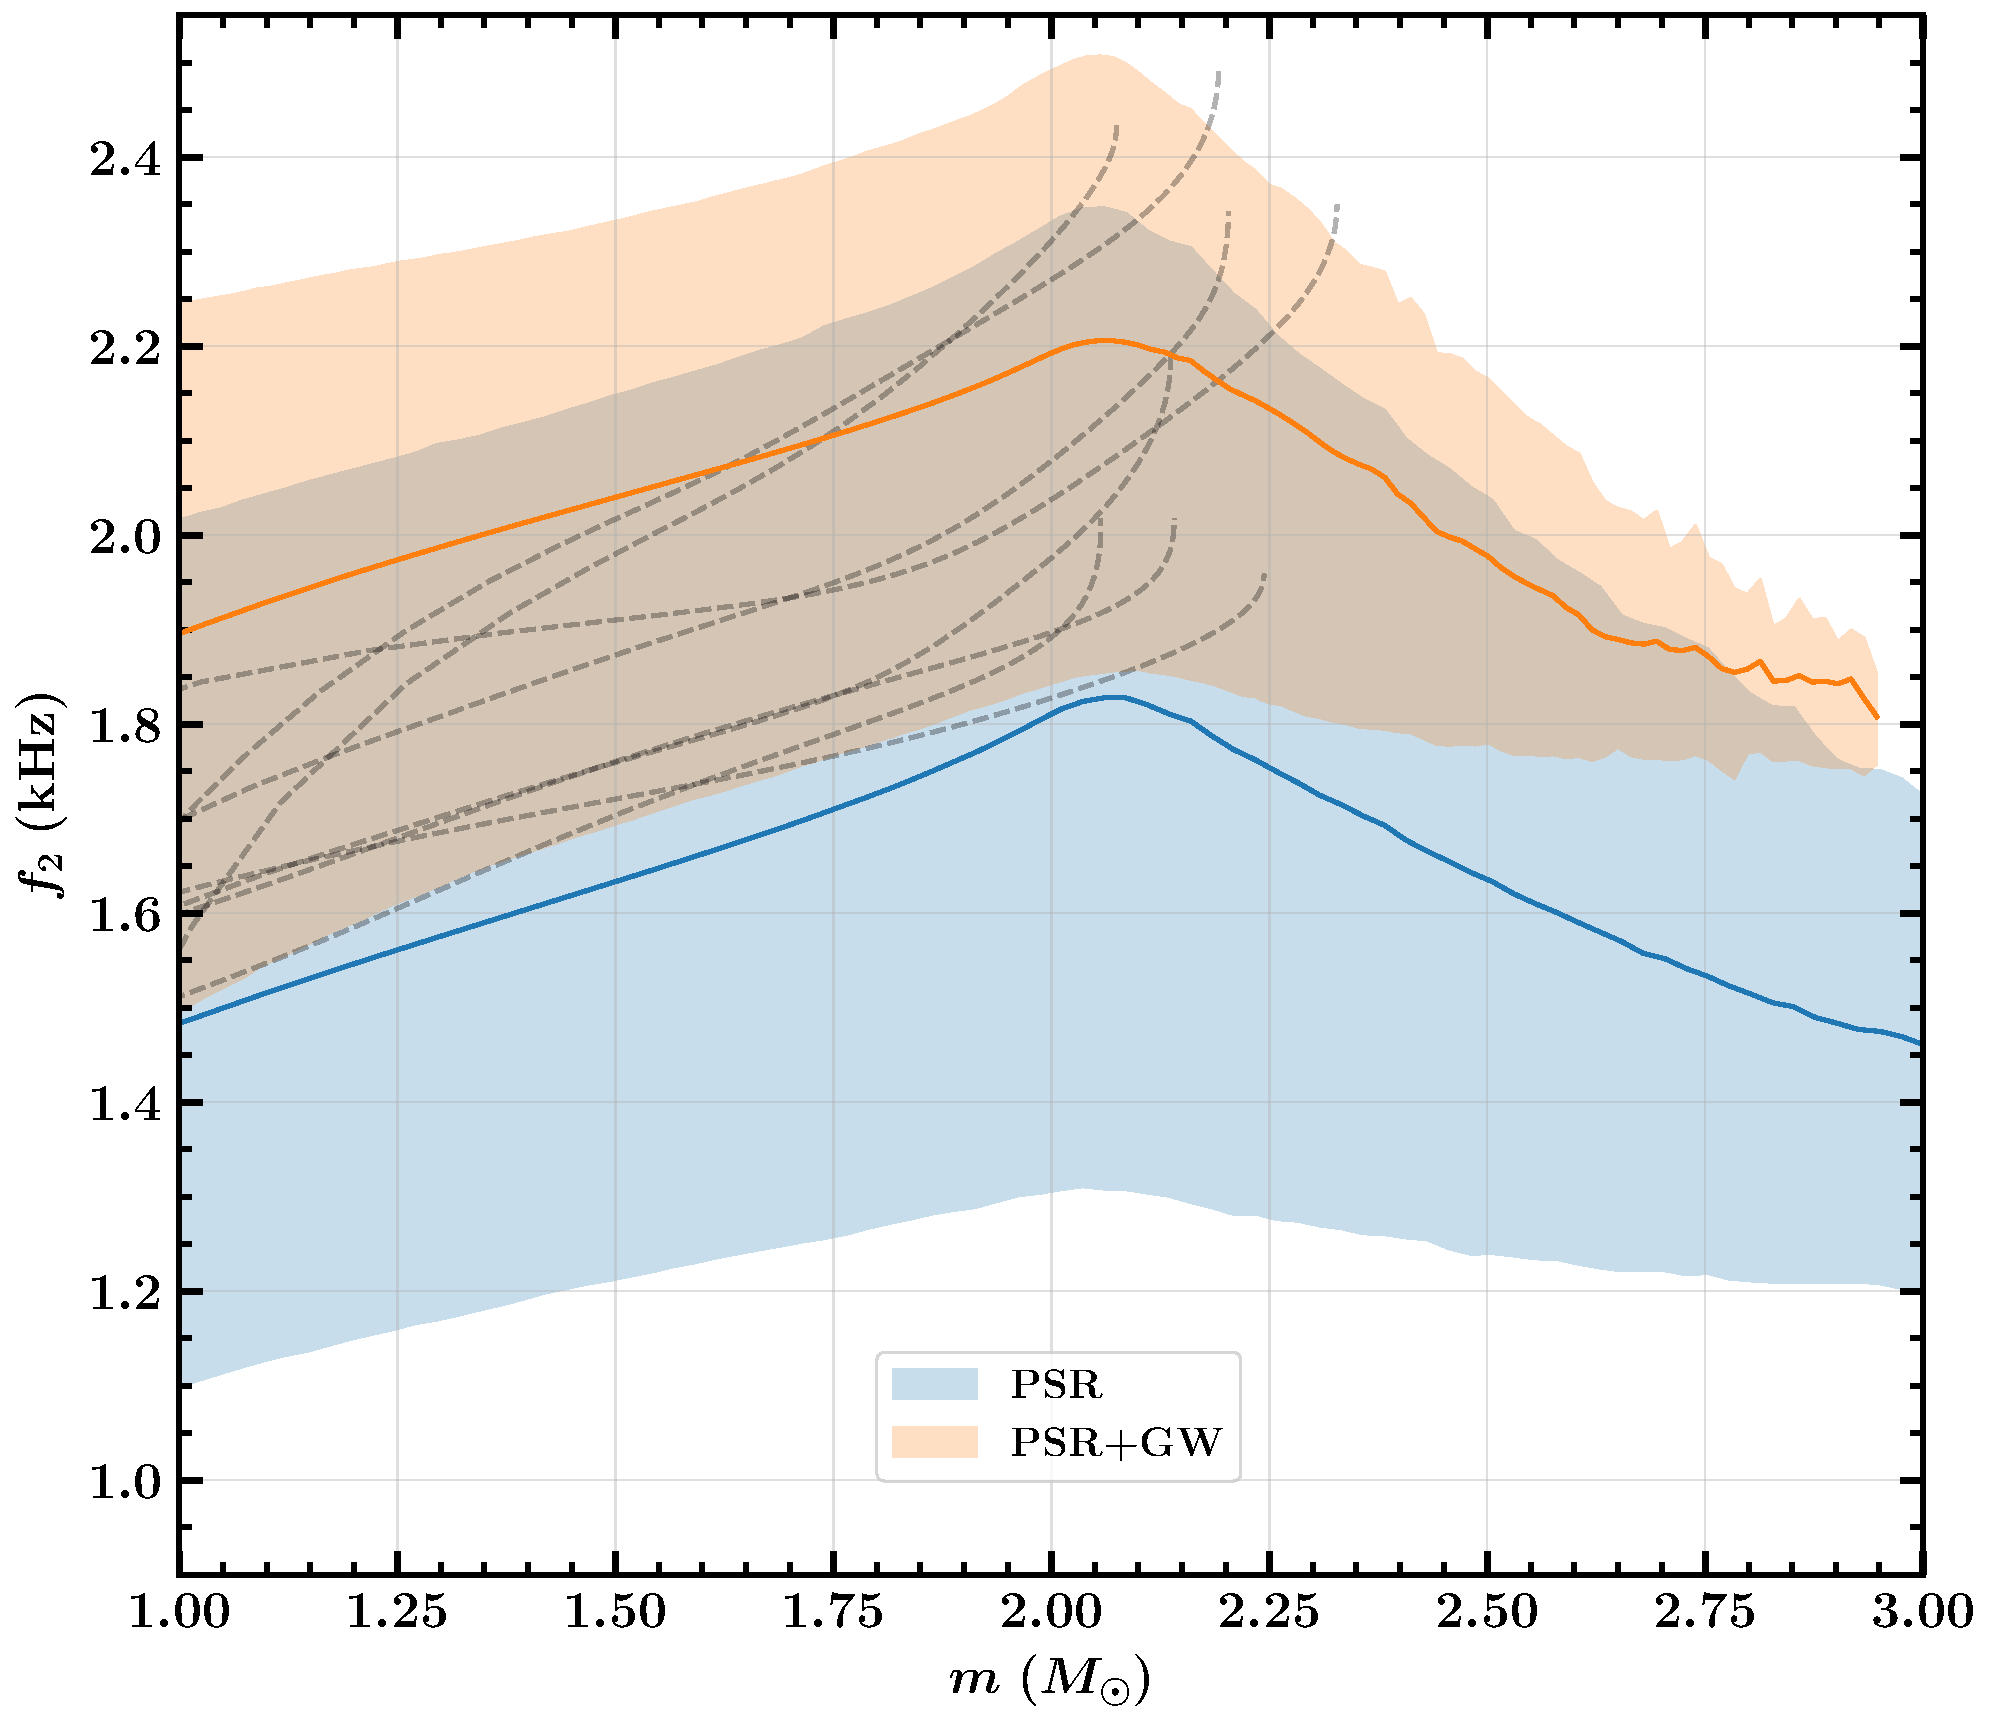
\includegraphics[width=\linewidth]{Full_GR/Envelope_plot1.pdf} \\
    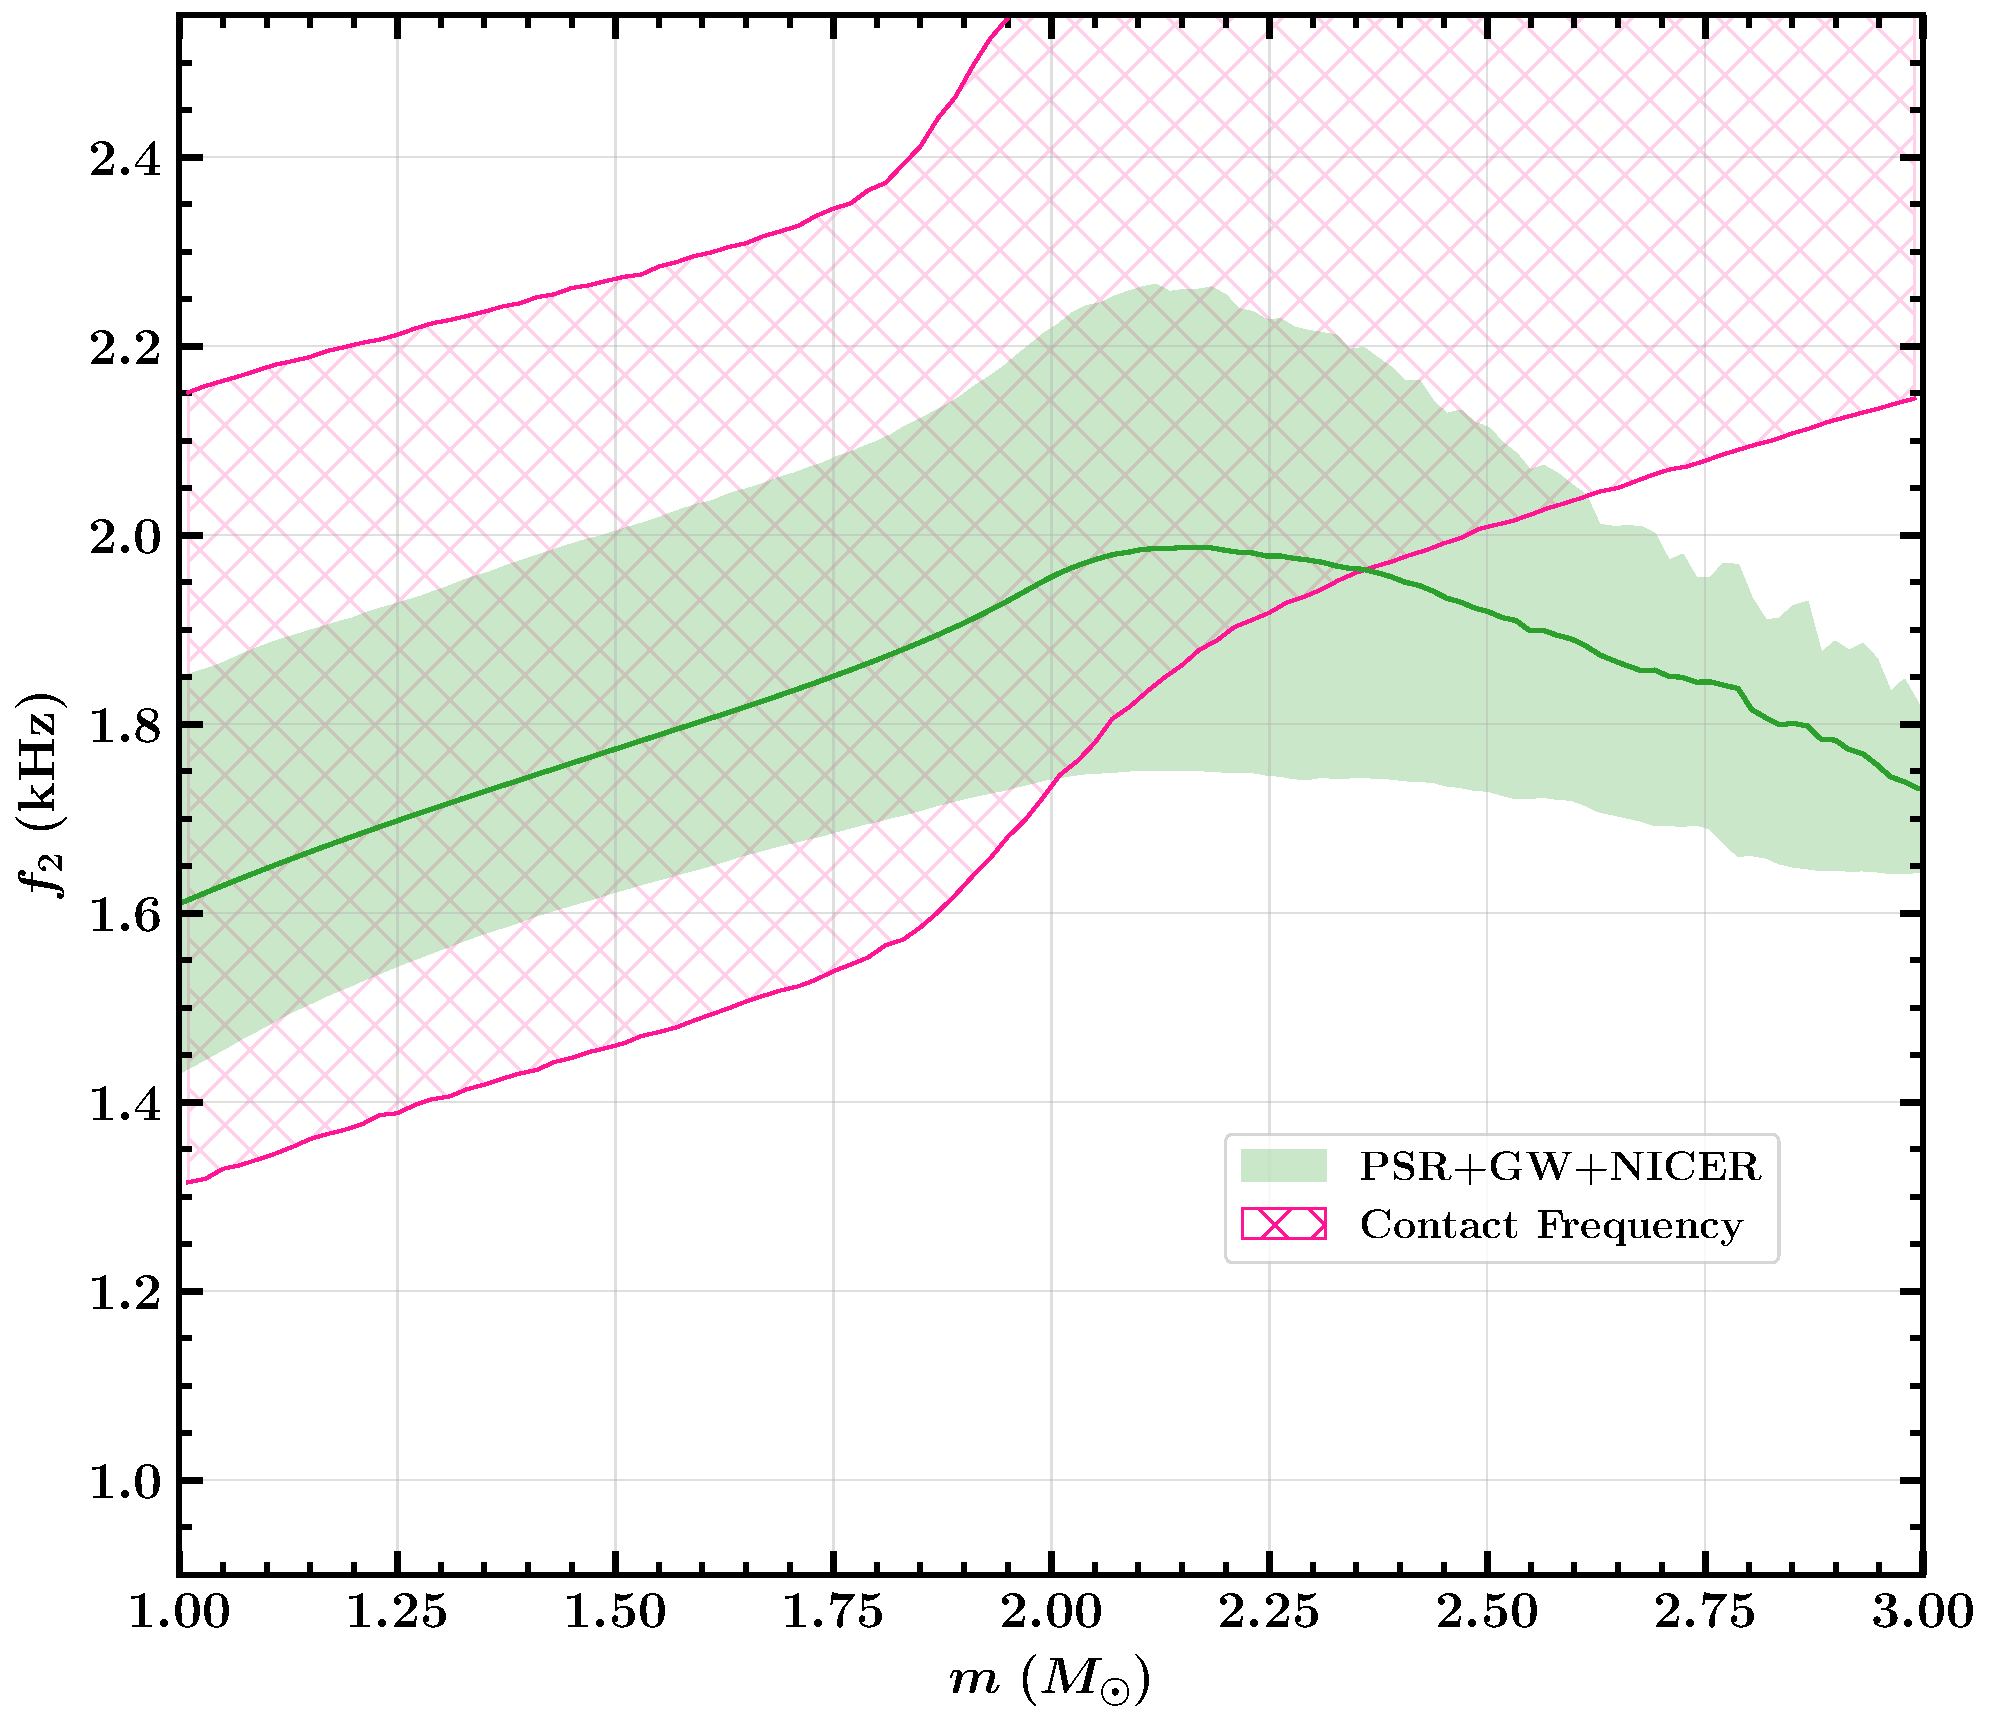
\includegraphics[width=\linewidth]{Full_GR/Envelope_plot2.pdf}
    \caption{Mean (solid line) quadrupolar $f$-mode frequency and symmetric 90\% confidence interval (shaded) as a function of neutron star mass as inferred from PSR (\textit{top}), PSR+GW (\textit{top}), and PSR+GW+NICER (\textit{bottom}) datasets. Every realization (grey traces) of the $f_2(m)$ relation (\textit{top}) is monotonically increasing, but the mean of the distribution turns over above $2\,M_\odot$ because the EOSs that support larger neutron star masses are stiffer than average and thus have systematically lower $f_2$. The inferred $f_2(m)$ distributions are compared against the distribution of gravitational-wave contact frequencies $f_c$ (\textit{bottom}) expected for a realistic population of binary neutron star mergers: resonance of the $f$-mode with the orbital frequency can only occur if $f_2 < f_c$. \PL{Split into two, first plot loses pink shading and half of grey traces; pink shading + green contour + mean go on second plot} 
    \PL{Also, we should check the $f_2$ vs $f_c$ comparison very carefully}
    \SRM{I chose not to include the NICER estimates in the first plot to avoid clutter.}
    }
    \label{fig:Envelope Plot}
\end{figure}
%%%%%%%%%%%%%%

Computing the quadrupolar $f$-mode frequency as a function of neutron star mass for each EOS realization in the PSR, PSR+GW and PSR+GW+NICER datasets, we infer the distribution of $f_2(m)$ relations illustrated in Fig.~\ref{fig:Envelope Plot}, which depicts the mean and 90\% symmetric credible interval. The relation for each EOS is truncated at its TOV mass, $ M_{\rm TOV} $. The constraints are progressively refined as the different observations---PSR, GW and NICER---are sequentially incorporated. The broad extent of the PSR-conditioned distribution reflects the large uncertainty in $f_2(m)$ predictions when predicated only on the existence of $2\,M_\odot$ pulsars, besides basic physical considerations like causality and thermodynamic stability of the EOS. The addition of GW data shifts and tightens the distribution significantly, excluding stiffer EOSs that favor lower $f$-mode frequencies, especially at the intermediate mass scale probed by GW170817. These stiff EOSs are unable match the gravitational-wave measurements of neutron star tidal deformability. The inclusion of NICER data red-shifts and further narrows the distribution, particularly impacting the upper bound on $f_2(m)$: the stellar radii inferred from the pulse profile modeling exclude softer EOSs that produce more compact neutron stars with higher $f$-mode frequencies.

Within each dataset, we observe that the mean of the $f_2(m)$ distribution increases up until approximately $2\,M_\odot$, the minimum TOV mass compatible with the PSR data, and decreases thereafter. This is a feature of the distribution over $f_2(m)$ only, and not of individual $f_2(m)$ relations: as the $f$-mode frequency is intrinsically linked to the stellar compactness---which influences the speed at which perturbations propagate, and always increases with neutron star mass---$f_2(m)$ is a monotonically increasing function. The apparent decline in the mean $f_2(m)$ beyond $2\,M_\odot$ is simply a result of the diminishing number of EOSs capable of supporting such a large $M_{\rm TOV}$ being systematically stiffer than average.

%The $ f $-mode frequency is intrinsically linked to the internal structure of the NS, being particularly sensitive to both the compactness and radius of the star. The compactness, which is a measure of the star's gravitational strength, influences the speed at which perturbations propagate within the star, while the radius determines the extent of these perturbations. A higher compactness and smaller radius result in a higher $ f $-mode frequency. Thus, $f_2(m)$ is a monotonically increasing function of mass. This is reflected in the trend of the mean inferred $f_2(m)$ relation, which increases up to approximately $2 M_\odot$, the minimum TOV mass compatible with the PSR data, for all three datasets. Beyond this mass, the mean $f_2(m)$ decreases as a diminishing number of EOSs are capable of supporting such a large $M_{\rm TOV}$, leading to an apparent turnover in the frequency distribution. We emphasize, however, that individual realizations of $f_2(m)$ sampled from the distribution remain monotonically increasing.

\begin{comment}
We now shift our focus to comparing the f-modes with the frequency of contact during a GW merger. 
If the $f$-mode is comparable, or lower than the contact frequency, then the $f$-mode oscillations may achieve resonance with the binaries orbit before the merger (contact) \cite{Steinhoff_2016}. 
Consequently, the $f$-mode may imprint itself on the GWs emitted in the late stages of inspiral \cite{PhysRevLett.116.181101}. 
We study these effects using our updated constraints for the f-modes. 
First, we define the GW contact frequency using Agathos et al. \cite{Agathos_2015}. 
\begin{equation}
    f^{\mathrm{kepler}}_{\mathrm{contact}} = \sqrt{\frac{m_1 + m_2}{(r_1 + r_2)^3} \frac{G}{\pi^2}}
\end{equation}
This equation, using Kepler's laws calculates the orbital frequency at contact. Note that the dominant resonance for f-modes should be compared to twice the orbital frequency $2 f^{\mathrm{kepler}}_{\mathrm{orbit}} = f^{\mathrm{kepler}}_{\mathrm{contact}}$. 
However, the BNS may come into contact before this value is reached \cite{Agathos_2015}. 
To account for this we follow the Agathos et al. prescription of taking the minimum between the contact frequency $f_{\mathrm{contact}}$, and the frequency of the last stable circular orbit (LSO) $f_{\mathrm{LSO}}$. 
$f_{\mathrm{contact}} = \mathrm{min}(f_{\mathrm{LSO}}, f^{\mathrm{kepler}}_{\mathrm{contact}})$. 
Under this condition, $f_2 < f_{\mathrm{contact}}$ would imply that the f-mode achieves resonance within the binaries coalescence. 

In Fig.~\ref{fig:Envelope Plot}, we compare the quadrupolar $f$-mode frequency for a neutron star against the distribution of contact frequencies expected for a population of binary neutron star mergers. We find that the $f$-modes are comparable to the contact frequency of merger at all mass bins. Furthermore, at low-mass bins, the f-modes are consistently lower than their corresponding contact frequency. 
That is, for $1 M_{\odot} - 1 M_{\odot}$ mergers, the f-mode achieves resonance during the binaries inspiral. 
\end{comment}
%\PL{We should define the GW contact frequency here, and explain that the dominant resonance occurs when the orbital frequency is twice the $f$-mode frequency (i.e. GW frequency equal to $f$-mode frequency), such that $f_2 < f_c$ is the condition for achieving resonance; also, reading arXiv:2203.00623 I notice that the ISCO frequency is sometimes lower than $f_c$, so we might want to change our criterion to $f_2 < \mathrm{min}(f_c,f_{\rm ISCO})$. Let's discuss}


\BK{We now shift our focus to the comparison between the $f$-modes and the GW contact frequency during binary neutron star (BNS) mergers. The critical aspect of this comparison is to determine whether the $f$-mode frequency is comparable to or less than the contact frequency. If this condition holds, the $f$-mode oscillations can resonate with the binary's orbit prior to the stars making contact \cite{Steinhoff_2016}. Such resonance may leave a detectable signature on the gravitational waveforms emitted in the final stages of the inspiral \cite{PhysRevLett.116.181101}. To define the contact frequency, we employ the Keplerian expression as provided by Agathos et al. \cite{Agathos_2015}:}

\begin{equation}
f_{\text{contact}}^{\text{kepler}} = \sqrt{\frac{m_1 + m_2}{(r_1 + r_2)^3} \frac{G}{\pi^2}}, 
\end{equation}
,

\BK{where $m_1$ and $m_2$ denote the masses, and $r_1$ and $r_2$ represent the radii of neutron stars. This equation, utilizing Kepler's laws, calculates the orbital frequency at contact. It should be noted that the dominant resonance for the $f$-modes should be compared with twice the orbital frequency $2 f^{\mathrm{kepler}}_{\mathrm{orbit}} = f^{\mathrm{kepler}}_{\mathrm{contact}}$. However, the BNS system often merges before reaching this frequency. Therefore, the actual contact frequency is the lower value between the last stable circular orbit (LSO) frequency and the Keplerian contact frequency: $f_{\text{contact}} = \min(f_{\text{LSO}}, f_{\text{contact}}^{\text{kepler}})$. This criterion, $f_2 < f_{\text{contact}}$, implies that the $f$-mode may achieve resonance during the final inspiral stages, potentially influencing the observed gravitational wave signal.}


\BK{In Fig.~\ref{fig:Envelope Plot}, the quadrupolar $f$-mode frequency for a neutron star is compared against the distribution of contact frequencies for binary neutron star mergers. Across different mass bins, the $f$-mode frequencies are observed to be comparable to or lower than the contact frequencies. For lower-mass mergers, such as $1 M_\odot - 1 M_\odot$ binaries, the $f$-mode frequency is typically lower than the corresponding contact frequency, suggesting that resonance is achieved prior to merger. This resonance could substantially influence the gravitational waveforms observed during the inspiral phase, as the $f$-mode oscillations would imprint on the signal at frequencies relevant to current and future gravitational wave detectors. This is significant because resonance with the $f$ mode establishes a direct correlation between the gravitational wave signal and compactness and internal structure of the neutron star. The strong gravitational fields in compact neutron stars amplify the $f$-mode frequency, and this coupling with the orbital motion intensifies as the stars spiral closer together. Consequently, the detection of such resonances could help to constrain the EOS of dense matter\cite{PhysRevLett.116.181101}.}


%%%%%%%%%%%%%%%%%%%
\subsection{$f$-mode frequency estimates for individual neutron stars}
%%%%%%%%%%%%%%%%%%%

%%%%%%%%%%%%%%
\begin{figure}
    \centering
    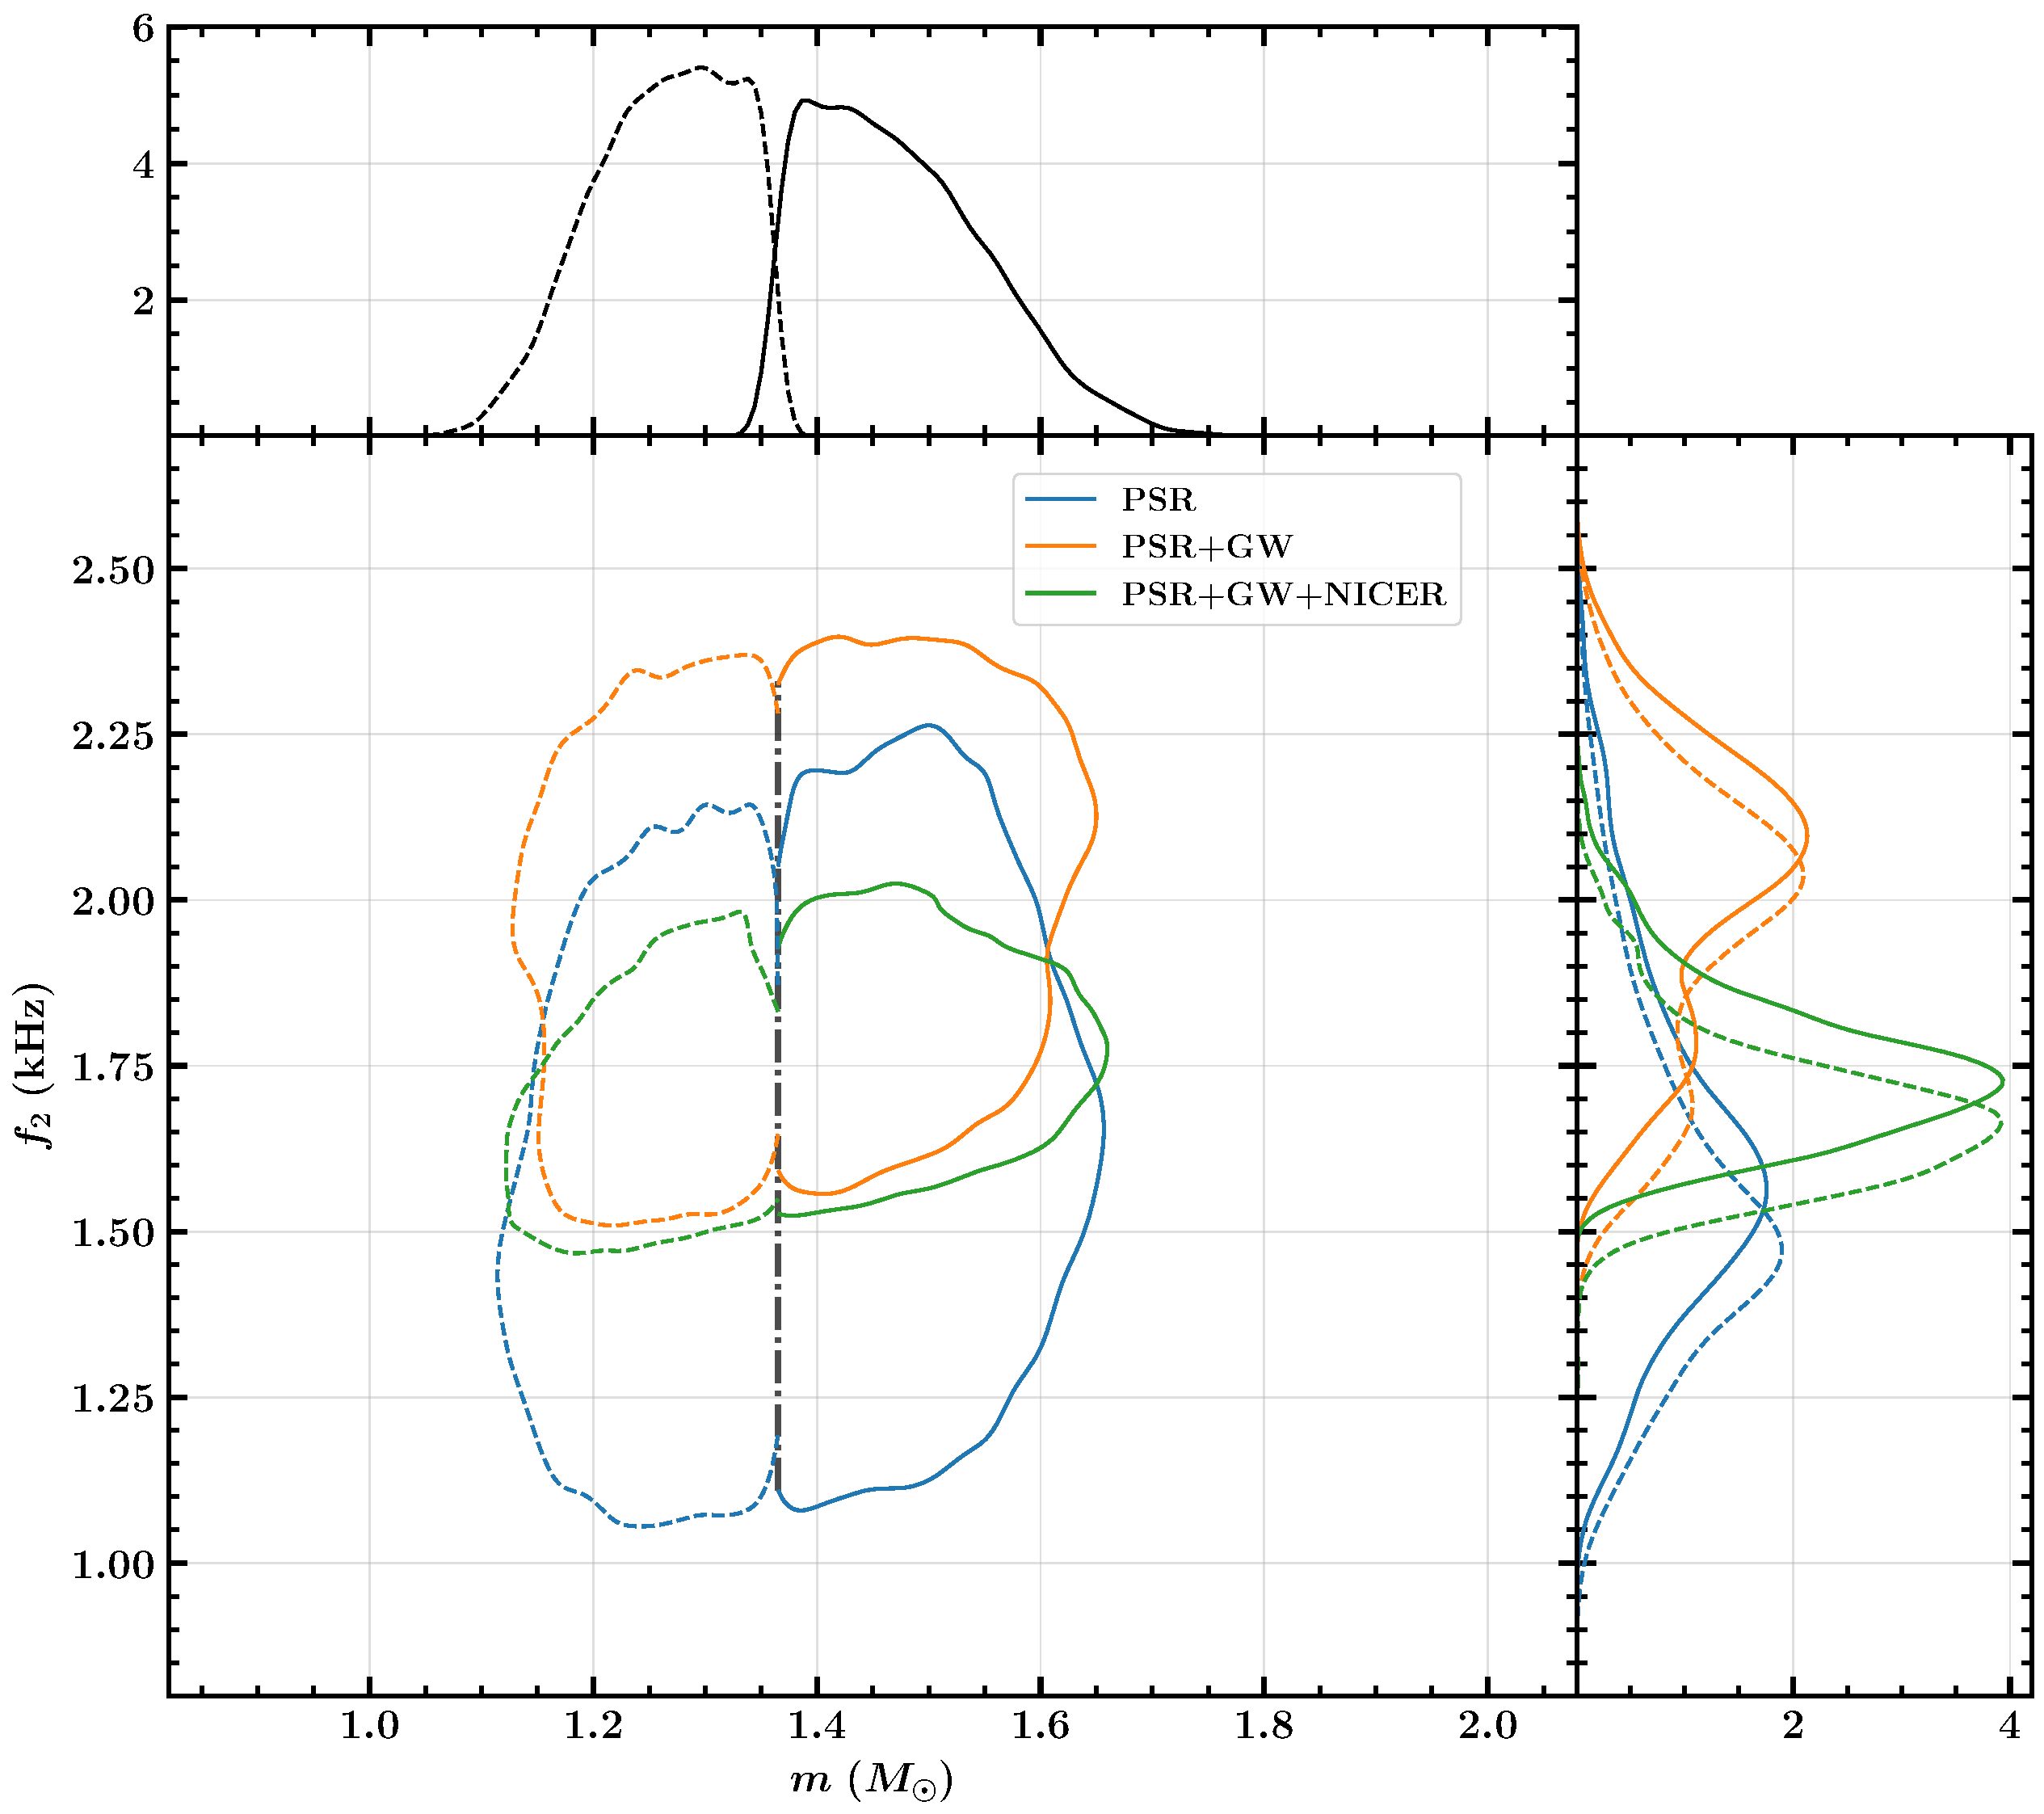
\includegraphics[width=\linewidth]{Full_GR/GW170817_2D_posterior.pdf}%
    \caption{Inferred two-dimensional marginal posterior distributions over mass and quadrupolar $f$-mode frequency for the primary and secondary components of GW170817 \cite{GW170817}. The distributions are conditioned on three different observational datasets. Contours delimit 90\% confidence regions.}
    \label{fig:GW170817_GW190425_2D_posterior}
\end{figure}
%%%%%%%%%%%%%%

%%%%%%%%%%%%%%
\begin{figure}
    \centering
    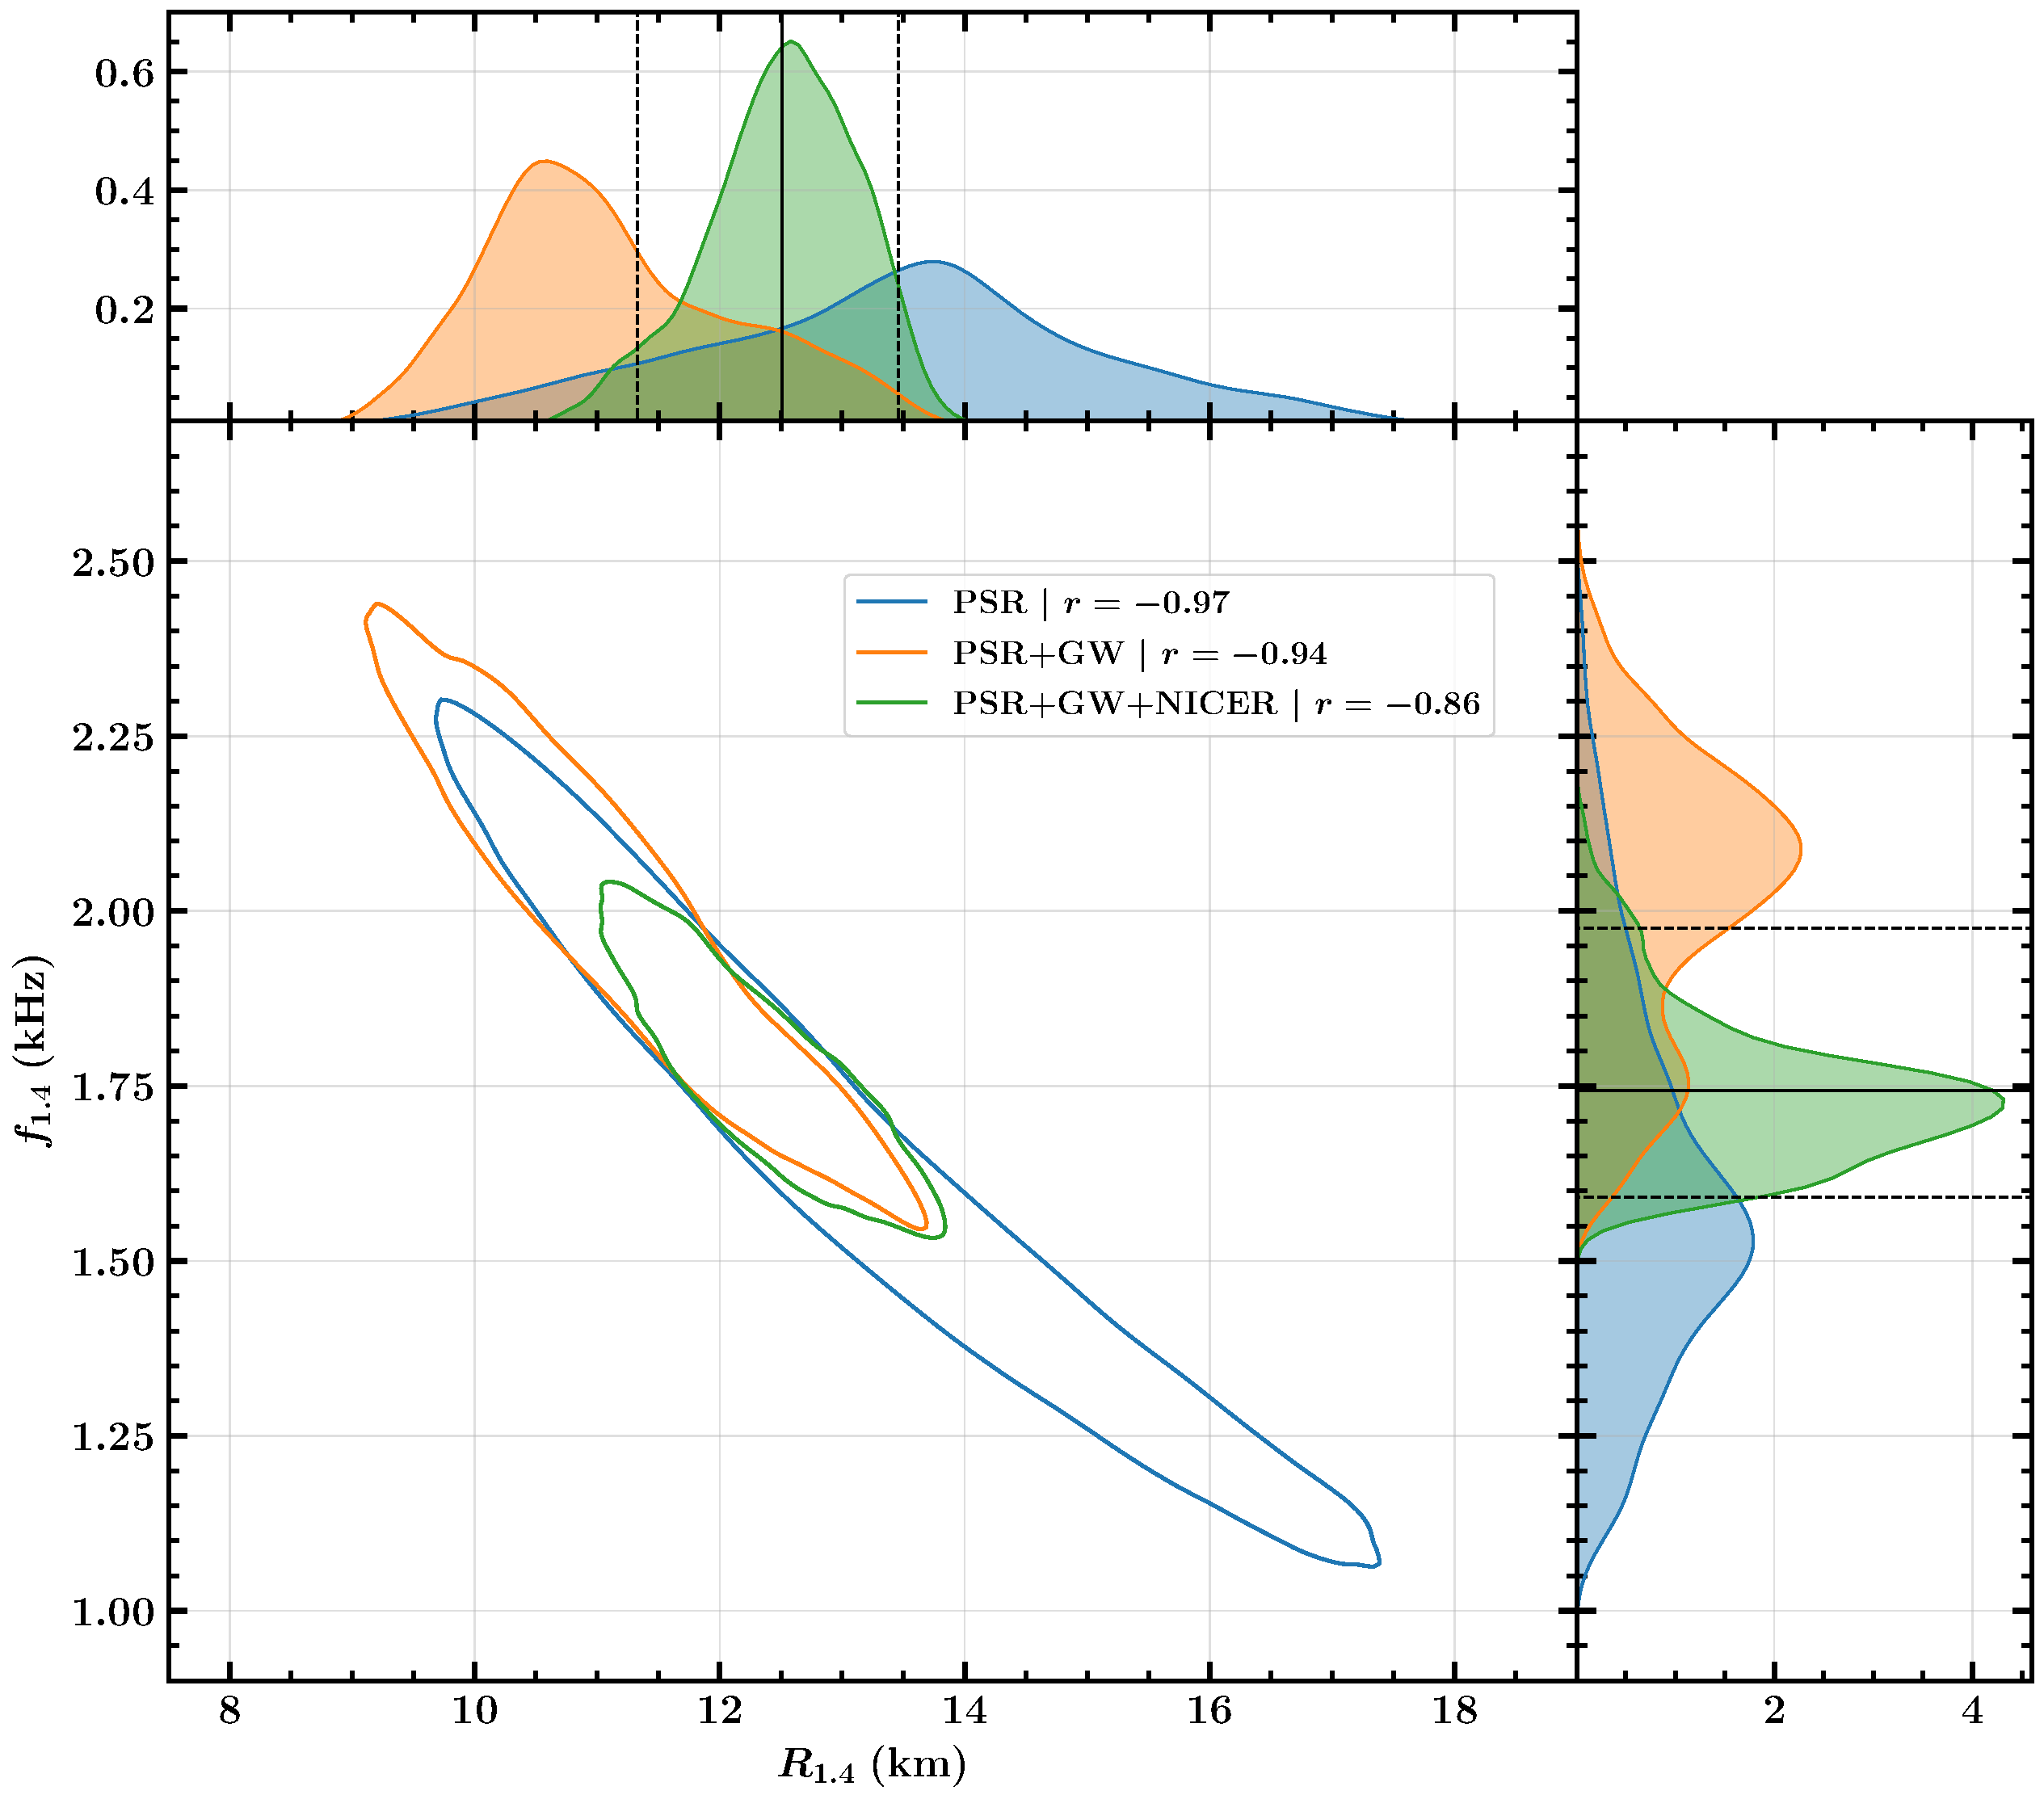
\includegraphics[width=\linewidth]{Full_GR/Canonical_distribution.pdf} \\
    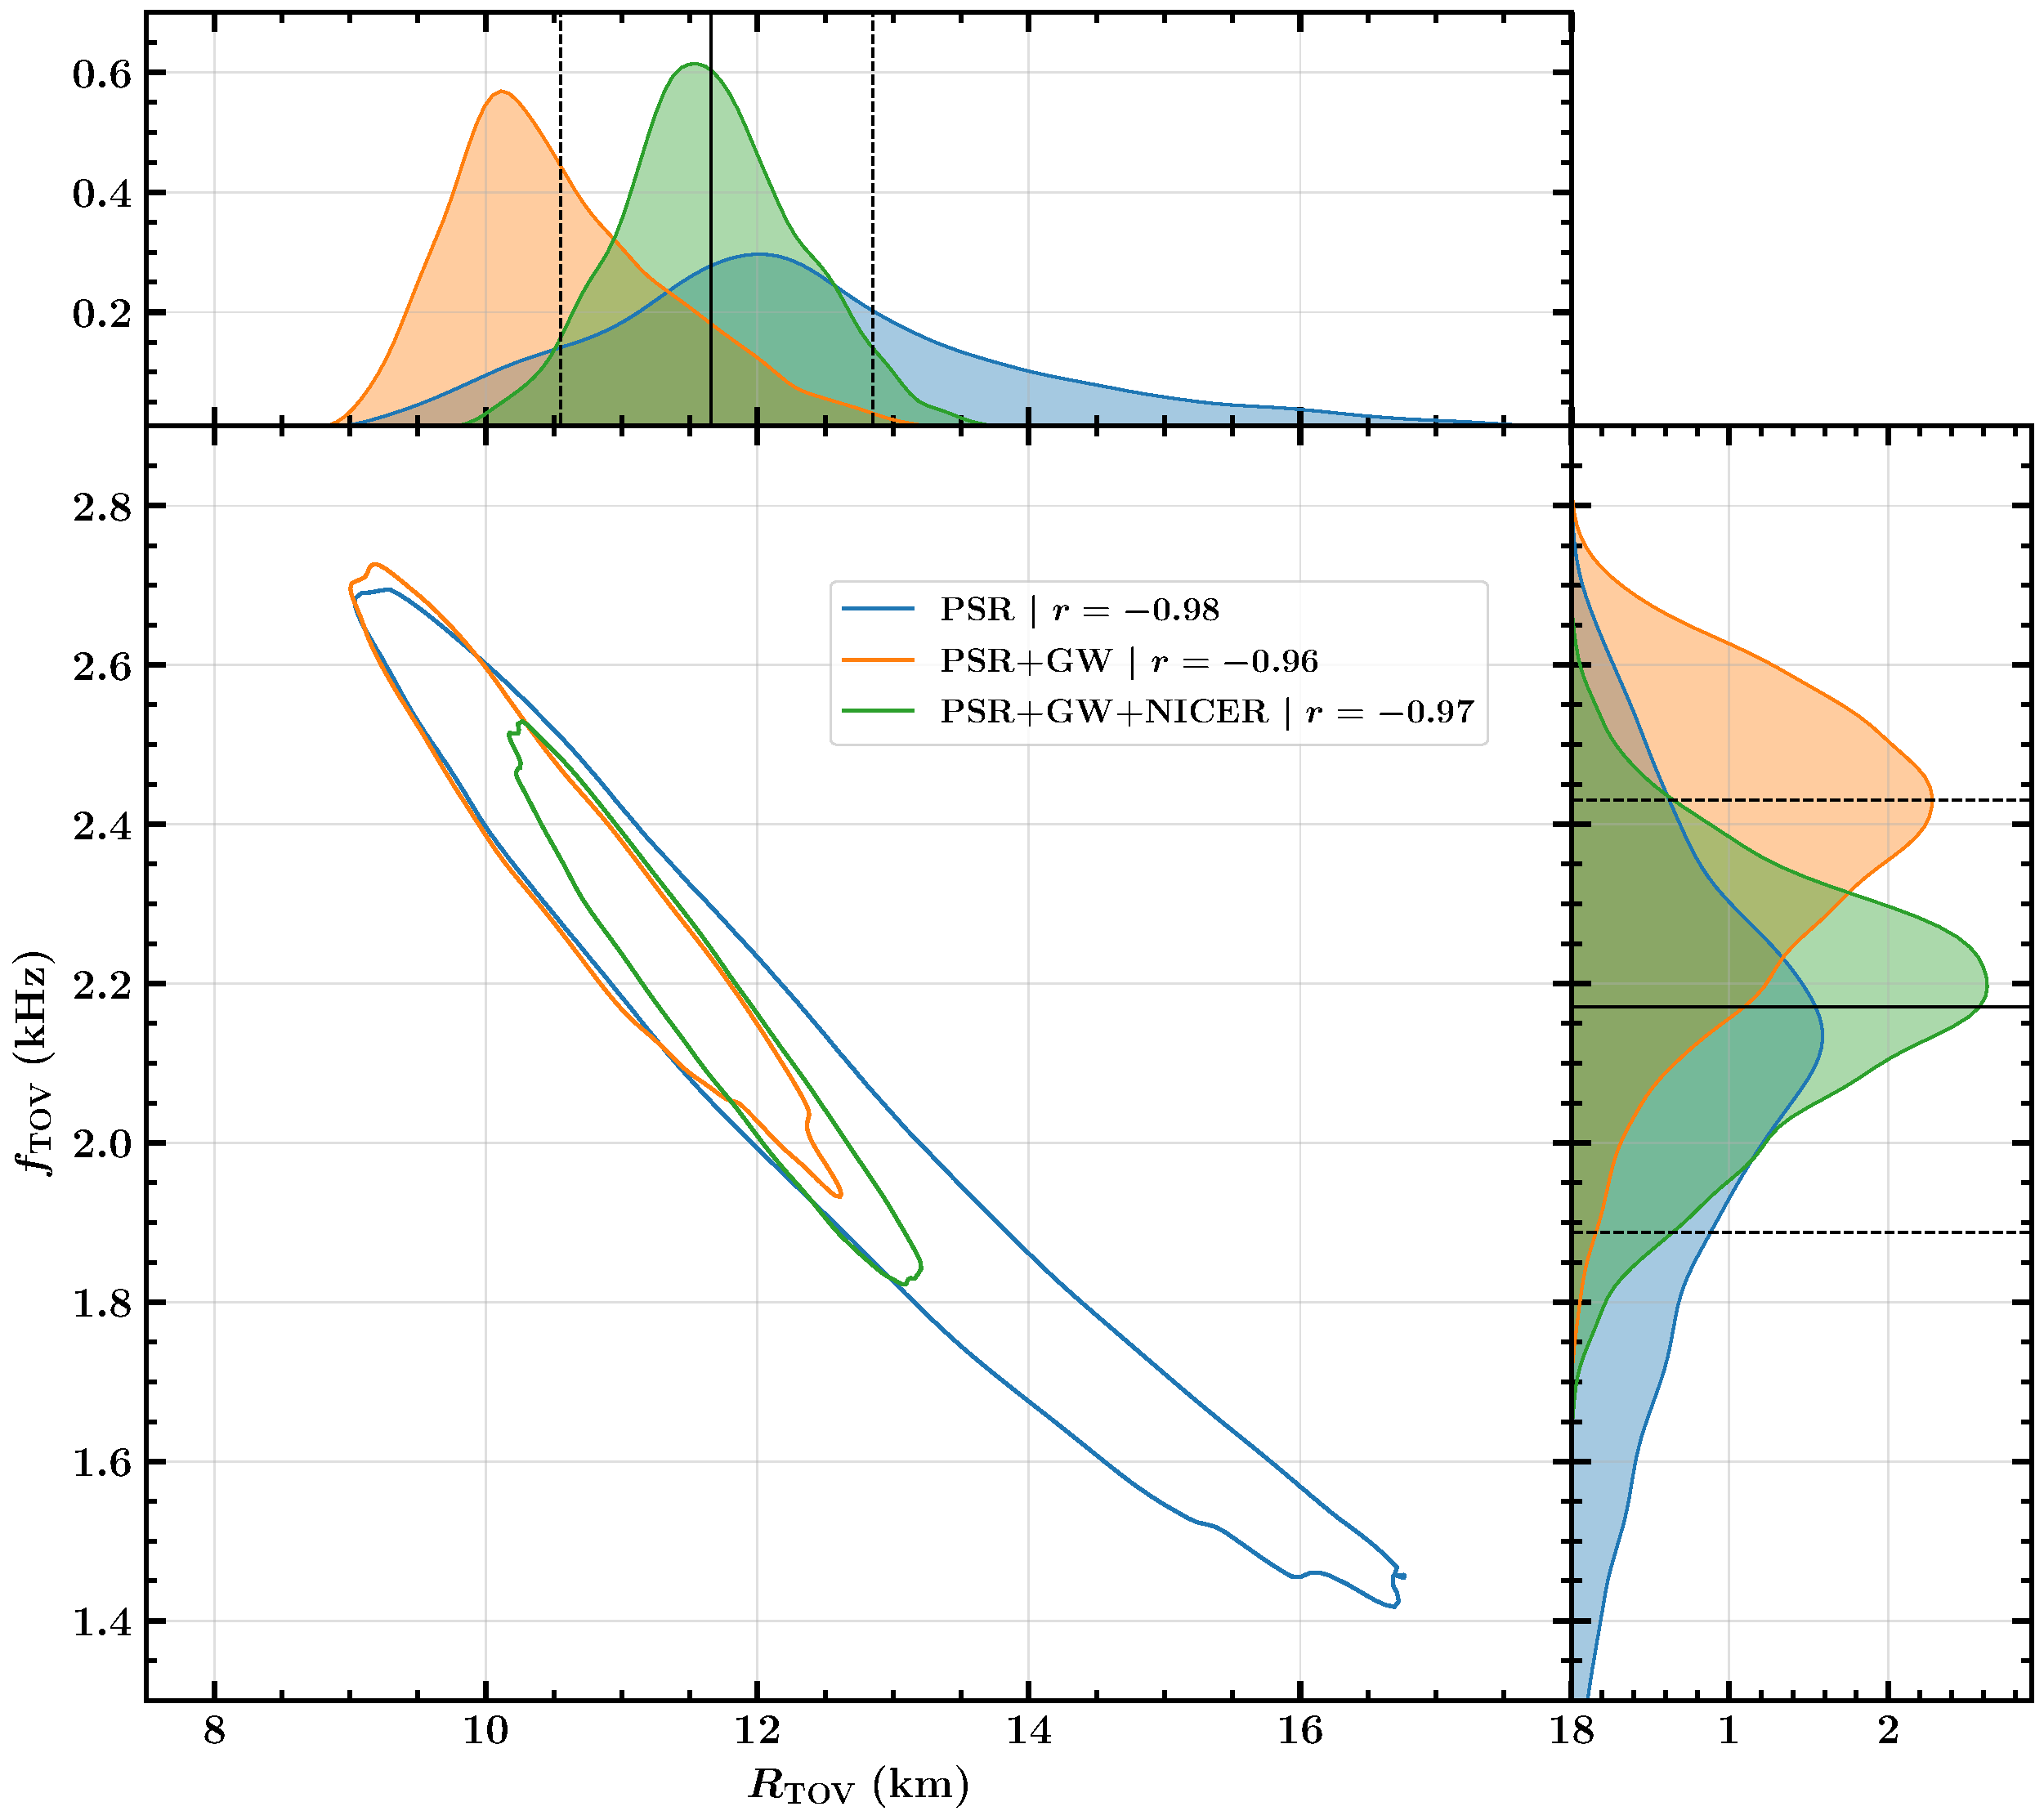
\includegraphics[width=\linewidth]{Full_GR/TOV_max_lim_Radius.pdf}
    \caption{Inferred two-dimensional marginal posterior distributions over radius for canonical neutron stars (\textit{top}) or TOV radius for maximum-mass neutron stars (\textit{bottom}) and corresponding quadrupolar $f$-mode frequency. The distributions are conditioned on three different observational datasets. Contours delimit 90\% confidence regions. The value of $f_{1.4}$ is strongly (anti-)correlated with $R_{1.4}$. A similar, with a high precise, correlation is observed between $f_{\rm TOV}$ and $R_{\rm TOV}$. The correlation coefficients are mentioned alongside the legends of respective dataset.
    \SRM{I have mentioned the correlation coefficients in the plots and replaced $M_{TOV}$ with $R_{TOV}$}
    }
    \label{fig:nsfmodes}
\end{figure}
%%%%%%%%%%%%%%

Evaluating the posterior on $f_2(m)$ at a given value of $m$, or marginalizing the distribution over an uncertain mass measurement, we predict the expected quadrupolar $f$-mode frequency for several specific neutron stars, as informed by each observational dataset. In Table~\ref{tab:nsfmodes}, we list the estimated $f_2$ value for canonical $1.4 M_\odot$ neutron stars, TOV stars, and the neutron star components of the compact binary mergers observed by the LIGO-Virgo-KAGRA collaboration to date. In particular, we consider the primary and secondary components of the binary neutron star mergers GW170187~\cite{GW170817} and GW190425~\cite{GW190425}, as well as the secondary components of the neutron-star--black-hole mergers GW200105, GW200115 and GW230529 \cite{GW200105_GW200115,GW230529}. Quoted symmetric 90\% credible intervals about the mean account for the uncertainty in the $f_2(m)$ relation. The error in $f_{\rm TOV}$ also incorporates the uncertainty in the value of $M_{\rm TOV}$ inferred from each dataset.

Figure~\ref {fig:GW170817_GW190425_2D_posterior} focuses on the predictions for GW170817, illustrating the two-dimensional marginalized posterior distributions over the masses $ m_{1,2} $ and quadrupolar $ f $-mode frequencies $ f_2^{(1,2)} $ of the compact binary's components. The posteriors are conditioned on the three different observational datasets, progressively incorporating PSR, GW, and NICER observations. Each observational dataset incrementally improves the precision of the $f$-mode frequency estimates. The hierarchy $m_1 \geq m_2$ of the component masses enforces a hierarchy $f_2^{(1)} \geq f_2^{(2)}$, which is not apparent in the contour plot or the one-dimensional marginal distributions, when a universal EOS is imposed.

We also investigate the correlations between pairs of these observables. The marginal two-dimensional posteriors on $R_{1.4}$ and $f_{1.4}$, and on $R_{\rm TOV}$ and $f_{\rm TOV}$, are plotted in Fig.~\ref{fig:nsfmodes} for the three observational datasets considered. We observe a strong (anti-)correlation between $R_{1.4}$ and $f_{1.4}$ in the top panel: larger-radius neutron stars are less compact, giving them lower $f$-mode frequencies. The constraining effect of GW and NICER observations, relative to the PSR data, is to disfavor EOSs that prefer large- and small-radius neutron stars, respectively. Because of the strong correlation with $f_{1.4}$, these observations significantly limit the range of allowed values for the quadrupolar $f$-mode frequency of a canonical neutron star. \todo{The lower panel exhibits a similar with a stronger (anti-)correlation between $ R_{\text{TOV}} $ and $ f_{\text{TOV}}$...}

%The left panel illustrates how the inclusion of data from different sources impacts our understanding of the relationship between the radius $ R_{1.4} $ and the quadrupolar $ f $-mode frequency $ f_{1.4}$ of a canonical $1.4 M_\odot$ neutron star. Initially, the blue contours, representing PSR data alone, show a wide spread with $ R_{1.4} $ ranging from approximately 11.5 km to 14.5 km and $ f_{1.4} $ ranging from around 1.4 kHz to 2.3 kHz. With the inclusion of GW data (orange contours), the distribution narrows, particularly along the radius axis. The GW data mainly exclude stiffer EOSs, which predict larger radii and lower $ f_{1.4} $ frequencies. As a result, the credible region tightens, with $ R_{1.4} $ now constrained to a range of approximately 12.5 km to 13.5 km, and $ f_{1.4} $ frequencies are refined to lie between 1.5 kHz and 2.1 kHz. Finally, the green contours (PSR+GW+NICER) represent the most constrained distribution, with $ R_{1.4} $ now narrowed to a range of about 12.7 km to 13.3 km, and $ f_{1.4} $ constrained to between 1.7 kHz and 2.0 kHz. \PL{[Are these the 90\% credible intervals?]}\BK{Yes, all the values mentioned in the discussion based on 90\%  credible intervals but still @Sailesh can verify these numbers with his code. } The reduction in uncertainty is a direct consequence of the strong correlation between the star's radius and its $ f $-mode frequency: a smaller radius typically results in higher compactness, leading to higher $ f $-mode frequencies due to the stronger gravitational potential and reduced perturbation travel time across the star.

We also explored the correlation between $ M_{\text{TOV}} $ and $ f_{\text{TOV}}$ and found out that in this case, however, the correlation is not as tight as $ R_{\text{TOV}} $ and $ f_{\text{TOV}}$ correlation, so the constraints on $M_{\rm TOV}$ do not restrict the allowed range of $f_{\rm TOV}$ values as sharply. Nonetheless, the effect of the GW and NICER observations, relative to the PSR data, is again to disfavor the stiffest (largest $M_{\rm TOV}$) and softest (smallest $M_{\rm TOV}$) EOSs, respectively. \PL{Check this explanation -- I suspect there's a strong correlation with $R_{\rm TOV}$. Let's discuss replacing the $M_{\rm TOV}$ plot with the $R_{\rm TOV}$ one}. \SRM{I agree to replace the $M_{\rm TOV}$ plot with the $R_{\rm TOV}$ one; however, we can still discuss the $M_{\rm TOV}$ correlation in the text.} 

%%%%%%%%%%%%
% \begin{table}
%     \centering
%     \caption{ \SRM{Correlation coefficients} \PL{Blend into text or show on figures; or else add caption and refer to it in the text}
%     }
%     \setlength{\tabcolsep}{2mm}
%     \renewcommand{\arraystretch}{2}
%     \scalebox{0.8}{
%         \begin{tabular}{lccc}
%             \hline \hline 
%             Dataset & PSR & PSR+GW & PSR+GW+NICER \\
%             \hline 
%             $M_{\rm TOV}-f_{\rm TOV}$ & $-0.582432$ & $-0.580644$ & $-0.394282$ \\
%             $R_{\rm TOV}-f_{\rm TOV}$ & $-0.977360$ & $-0.962087$ & $-0.970490$ \\
%             $R_{1.4}-f_{1.4}$ & $-0.969436$ & $-0.941340$ & $-0.860036$ \\
%             \hline \hline
%         \end{tabular}}
%     \label{tab:nsfmodes}
% \end{table}
%%%%%%%%%%%%
%The progression from PSR data alone (blue contours) to the combined PSR+GW+NICER data (green contours) mirrors the trend observed in the left panel. Initially, with only PSR data, the credible interval for $ M_{\text{max}} $ is broad, with values ranging from about 2.1 $ M_\odot $ to 2.8 $ M_\odot $, while the $ f_{\text{max}} $ spans from approximately 1.5 kHz to 2.3 kHz. This wide interval reflects significant uncertainty regarding the stiffness of the EOS at high densities, which directly influences both the TOV mass and $f_{\rm TOV}$. When GW data are incorporated (orange contours), the range of allowed $ M_{\text{max}} $ values narrows to approximately 2.2 $ M_\odot $ to 2.6 $ M_\odot $, with corresponding $ f_{\text{max}} $ frequencies refined to between 1.7 kHz and 2.2 kHz. Finally, the NICER data (green contours) provide further constraints, reducing the credible interval for $ M_{\text{max}} $ to a range of about 2.3 $ M_\odot $ to 2.5 $ M_\odot $, with $ f_{\text{max}} $ frequencies now tightly constrained between 1.8 kHz and 2.1 kHz. \PL{[Are these 90\% confidence intervals as well?]} We observe that $f_{\rm TOV}$ is less strongly correlated with $M_{\rm TOV}$ compared to $f_{1.4}$ and $R_{1.4}$.

%As was done for $f_{\rm TOV}$, we can also predict the quadrupolar $f$-mode frequencies for individual neutron stars observed in compact binary mergers, marginalizing over uncertainty in their component mass. In Table~\ref{tab:Event_estimates}, we list the predicted $f_2$ values and uncertainties for components of GW170817 and GW190425, as well as the lighter components of GW200105, GW200115 and GW230529. Figure~\ref {fig:GW170817_GW190425_2D_posterior} illustrates the marginalized posterior distributions for the masses $ m_{1,2} $ and quadrupolar $ f $-mode frequency $ f_2^{(1,2)} $ of the individual components in the binary neutron star mergers GW170817 (left panel) and GW190425 (right panel). These events are analyzed through three different observational data sets---PSR, GW, and NICER measurements---each incrementally improving the precision of our estimates. For GW170817, the left panel shows that the primary (blue) and secondary (orange) components have mass distributions initially centered around $ 1.4 \, M_\odot $ and $ 1.2 \, M_\odot $, respectively, with corresponding $ f $-mode frequencies ranging broadly from approximately 1.2 kHz to 2.1 kHz. The broadness of these distributions reflects significant initial uncertainties, particularly when only PSR data are considered. However, as GW data are incorporated, the mass distributions narrow significantly, particularly constraining the primary mass to the range $ 1.36 \, M_\odot $ to $ 1.54 \, M_\odot $, and the corresponding $ f_1 $ frequency is refined to between 1.6 kHz and 2.0 kHz. Similarly, the secondary mass is confined to $ 1.16 \, M_\odot $ to $ 1.36 \, M_\odot $, with the $ f_2 $ frequency range narrowed to 1.5 kHz to 1.9 kHz. These constraints arise because GW observations provide key information about the tidal deformability, which is sensitive to the neutron star’s EOS and thus rules out softer EOSs that would predict lower masses and frequencies. The inclusion of NICER data, which offers precise radius measurements, further tightens these distributions. For instance, the primary component’s mass is now centered more narrowly around $ 1.4 \, M_\odot $, with a corresponding frequency between 1.7 kHz and 1.9 kHz, reflecting a strong constraint on the neutron star's compactness.

%In contrast, the right panel, which represents the GW190425 event, depicts a binary system with notably higher masses, emphasizing the distinct nature of this system compared to GW170817. The primary component of GW190425 (green) has an initial mass centered around $ 2.0 \, M_\odot $ with a wide $ f $-mode frequency distribution ranging from approximately 1.5 kHz to 2.25 kHz. The secondary component (red) shows a mass distribution centered around $ 1.6 \, M_\odot $, with frequencies ranging from 1.4 kHz to 2.1 kHz. When GW data are included, the primary mass $ M_1 $ is constrained to a narrower range between $ 1.9 \, M_\odot $ and $ 2.1 \, M_\odot $, and the corresponding $ f_1 $ frequency is refined to between 1.8 kHz and 2.1 kHz. The secondary component's mass is similarly constrained to $ 1.5 \, M_\odot $ to $ 1.7 \, M_\odot $, with a frequency range narrowed to 1.6 kHz to 1.9 kHz. The further inclusion of NICER data yields even tighter constraints, with the primary mass centered around $ 2.0 \, M_\odot $ and a frequency between 1.9 kHz and 2.0 kHz, while the secondary mass centers around $ 1.6 \, M_\odot $, with frequencies between 1.7 kHz and 1.8 kHz. These distributions highlight how GW190425’s higher mass components, compared to GW170817, correspond to higher $ f $-mode frequencies, reflecting the stronger gravitational fields and denser cores of these more massive neutron stars.  \PL{[Same question about credible intervals]}

\begin{comment}
%%%%%%%%%%%%
\begin{table}
    \centering
    \caption{Estimated quadrupolar $f$-mode frequency for selected neutron stars, as informed by different observational datasets. The mean and 90\% confidence interval for $f_2$ are quoted for a canonical 1.4 $M_\odot$ star, a maximum-mass TOV star, the primary and secondary components of the binary neutron star mergers GW170817 and GW190425, and the secondary components of the neutron-star--black-hole mergers GW200105, GW200115 and GW230529. Constraints on the canonical radius $R_{1.4}$ and the TOV mass $M_{\rm TOV}$ are also given. \SRM{[Isn't the dataset independent of GW observation in order to calculate mass distribution pdf? ($P(m|GW,dataset)=P(m|GW)$) As I don't find much difference in mass estimates of BNS components for different datasets.]}
    \PL{You're right, let's comment out masses in the table -- but maybe find a way to quote them in the text, so the reader doesn't have to look them up elsewhere}
    \SRM{I think it would be better to make two tables. One for GW binaries and the other for dataset parameters.}
    }
    \setlength{\tabcolsep}{2mm}
    \renewcommand{\arraystretch}{2}
    \scalebox{0.8}{
        \begin{tabular}{lccc}
            \hline \hline 
            Dataset & PSR & PSR+GW & PSR+GW+NICER \\
            \hline 
            $R_{1.4}$ (km) & $13.44^{+2.92}_{-2.94}$ & $11.11^{+1.92}_{-1.48}$ & $12.51^{+0.95}_{-1.18}$ \\
            $f_{1.4}$ (kHz) & $1.60^{+0.52}_{-0.41}$ & $2.01^{+0.31}_{-0.35}$ & $1.74^{+0.23}_{-0.15}$ \\
            $M_{\rm TOV}$ ($M_\odot$) & $2.33^{+0.59}_{-0.30}$ & $2.21^{+0.27}_{-0.18}$ & $2.25^{+0.35}_{-0.22}$ \\
            $R_{\rm TOV}$ (km) & $12.47^{+3.48}_{-2.48}$ & $10.58^{+1.59}_{-1.16}$ & $11.66^{+1.19}_{-1.11}$ \\
            $f_{\rm TOV}$ (kHz) & $2.06^{+0.46}_{-0.55}$ & $2.37^{+0.27}_{-0.34}$ & $2.17^{+0.26}_{-0.28}$ \\
            % GW170817 $m_{1}$ ($M_\odot$) & $1.48^{+0.14}_{-0.11}$ & $1.48^{+0.14}_{-0.11}$ & $1.48^{+0.14}_{-0.11}$ \\
            GW170817 $f_{2}^{(1)}$ (kHz) & $1.63^{+0.52}_{-0.41}$ & $2.02^{+0.31}_{-0.36}$ & $1.75^{+0.23}_{-0.16}$ \\
            % GW170817 $m_{2}$ ($M_\odot$) & $1.26^{+0.09}_{-0.11}$ & $1.26^{+0.09}_{-0.11}$ & $1.26^{+0.09}_{-0.11}$ \\
            GW170817 $f_{2}^{(2)}$ (kHz) & $1.56^{+0.52}_{-0.39}$ & $1.95^{+0.34}_{-0.38}$ & $1.68^{+0.24}_{-0.16}$ \\
            % GW190425 $m_{1}$ ($M_\odot$) & $2.12^{+0.46}_{-0.42}$ & $2.12^{+0.46}_{-0.42}$ & $2.12^{+0.46}_{-0.42}$ \\
            GW190425 $f_{2}^{(1)}$ (kHz) & $1.84^{+0.50}_{-0.50}$ & $2.16^{+0.32}_{-0.35}$ & $1.96^{+0.29}_{-0.24}$ \\
            % GW190425 $m_{2}$ ($M_\odot$) & $1.33^{+0.27}_{-0.23}$ & $1.33^{+0.27}_{-0.23}$ & $1.33^{+0.27}_{-0.23}$ \\
            GW190425 $f_{2}^{(2)}$ (kHz) & $1.58^{+0.54}_{-0.42}$ & $1.97^{+0.34}_{-0.38}$ & $1.70^{+0.24}_{-0.19}$ \\
            % GW200105 $m_{2}$ ($M_\odot$) & $1.91^{+0.34}_{-0.24}$ & $1.91^{+0.34}_{-0.24}$ & $1.91^{+0.34}_{-0.24}$ \\
            GW200105 $f_{2}^{(2)}$ (kHz) & $1.83^{+0.54}_{-0.48}$ & $2.18^{+0.32}_{-0.37}$ & $1.93^{+0.29}_{-0.23}$ \\
            % GW200115 $m_{2}$ ($M_\odot$) & $1.54^{+0.75}_{-0.40}$ & $1.54^{+0.75}_{-0.40}$ & $1.54^{+0.75}_{-0.40}$ \\
            GW200115 $f_{2}^{(2)}$ (kHz) & $1.66^{+0.56}_{-0.45}$ & $2.04^{+0.36}_{-0.40}$ & $1.78^{+0.34}_{-0.23}$ \\
            % GW230529 $m_{2}$ ($M_\odot$) & $1.48^{+0.51}_{-0.29}$ & $1.48^{+0.51}_{-0.29}$ & $1.48^{+0.51}_{-0.29}$ \\
            GW230529 $f_{2}^{(2)}$ (kHz) & $1.64^{+0.55}_{-0.44}$ & $2.03^{+0.35}_{-0.39}$ & $1.76^{+0.29}_{-0.20}$ \\
            \hline \hline
        \end{tabular}}
    \label{tab:nsfmodes}
\end{table}
%%%%%%%%%%%%
\end{comment}

%%%%%%%%%%%%
\begin{table}
    \centering
    \caption{The mean and 90\% confidence interval for $f_2$ are quoted for a canonical 1.4 $M_\odot$ star, a maximum-mass TOV star as imposed by different observational datasets. Constraints on the canonical radius $R_{1.4}$ and the TOV mass $M_{\rm TOV}$ are also given.
    }
    \setlength{\tabcolsep}{2mm}
    \renewcommand{\arraystretch}{2}
    \scalebox{0.8}{
        \begin{tabular}{lccc}
            \hline \hline 
            Dataset & PSR & PSR+GW & PSR+GW+NICER \\
            \hline 
            $R_{1.4}$ (km) & $13.44^{+2.92}_{-2.94}$ & $11.11^{+1.92}_{-1.48}$ & $12.51^{+0.95}_{-1.18}$ \\
            $f_{1.4}$ (kHz) & $1.60^{+0.52}_{-0.41}$ & $2.01^{+0.31}_{-0.35}$ & $1.74^{+0.23}_{-0.15}$ \\
            $M_{\rm TOV}$ ($M_\odot$) & $2.33^{+0.59}_{-0.30}$ & $2.21^{+0.27}_{-0.18}$ & $2.25^{+0.35}_{-0.22}$ \\
            $R_{\rm TOV}$ (km) & $12.47^{+3.48}_{-2.48}$ & $10.58^{+1.59}_{-1.16}$ & $11.66^{+1.19}_{-1.11}$ \\
            $f_{\rm TOV}$ (kHz) & $2.06^{+0.46}_{-0.55}$ & $2.37^{+0.27}_{-0.34}$ & $2.17^{+0.26}_{-0.28}$ \\
            \hline \hline
        \end{tabular}}
    \label{tab:nsfmodes2}
\end{table}
%%%%%%%%%%%%

%%%%%%%%%%%%
\begin{table*}
    \centering
    \caption{Estimated quadrupolar $f$-mode frequency for GW observed neutron stars that participated in binary mergers, as informed by different observational datasets. The mean and 90\% confidence interval for $f_2$ are quoted the primary and secondary components of the binary neutron star mergers GW170817 and GW190425, and the secondary components of the neutron-star--black-hole mergers GW200105, GW200115 and GW230529. The `*' mark indicates that the primary component of the binary merger is a black-hole which is beyond the scope of this paper.
    \SRM{If this table looks cluttered then we can stick to previous table and quote the masses in text.}
    }
    \setlength{\tabcolsep}{3mm}
    \renewcommand{\arraystretch}{2}
    \scalebox{0.8}{
        \begin{tabular}{lcccccccc}
            \hline \hline 
            & $m_{1}$ ($M_\odot$) & $m_{2}$ ($M_\odot$) & \multicolumn{2}{c}{PSR} & \multicolumn{2}{c}{PSR+GW} & \multicolumn{2}{c}{PSR+GW+NICER} \\
            \hline 
            & & & $f_{2}^{(1)}$ (kHz) & $f_{2}^{(2)}$ (kHz) & $f_{2}^{(1)}$ (kHz) & $f_{2}^{(2)}$ (kHz) & $f_{2}^{(1)}$ (kHz) & $f_{2}^{(2)}$ (kHz) \\
            \hline 
            GW170817 & $1.48^{+0.14}_{-0.11}$ & $1.26^{+0.09}_{-0.11}$ & $1.63^{+0.52}_{-0.41}$ & $1.56^{+0.52}_{-0.39}$ & $2.02^{+0.31}_{-0.36}$ & $1.95^{+0.34}_{-0.38}$ & $1.75^{+0.23}_{-0.16}$ & $1.68^{+0.24}_{-0.16}$ \\
            GW190425 & $2.12^{+0.46}_{-0.42}$ & $1.33^{+0.27}_{-0.23}$ & $1.84^{+0.50}_{-0.50}$ & $1.58^{+0.54}_{-0.42}$ & $2.16^{+0.32}_{-0.35}$ & $1.97^{+0.34}_{-0.38}$ & $1.96^{+0.29}_{-0.24}$ & $1.70^{+0.24}_{-0.19}$ \\
            GW200105 & * & $1.91^{+0.34}_{-0.24}$ & * & $1.83^{+0.54}_{-0.48}$ & * & $2.18^{+0.32}_{-0.37}$ & * & $1.93^{+0.29}_{-0.23}$ \\
            GW200115 & * & $1.54^{+0.75}_{-0.40}$ & * & $1.66^{+0.56}_{-0.45}$ & * & $2.04^{+0.36}_{-0.40}$ & * & $1.78^{+0.34}_{-0.23}$ \\
            GW230529 & * & $1.48^{+0.51}_{-0.29}$ & * & $1.64^{+0.55}_{-0.44}$ & * & $2.03^{+0.35}_{-0.39}$ & * & $1.76^{+0.29}_{-0.20}$ \\
            \hline \hline
        \end{tabular}}
    \label{tab:nsfmodes}
\end{table*}
%%%%%%%%%%%%

%%%%%%%%%%%%%%%%%%%
\subsection{Distinguishability of $f$-modes}
%%%%%%%%%%%%%%%%%%%

Given the capability to produce EOS-informed predictions of $f_2$ for individual NSs, we examine the detectability of $f$-mode dynamical tides within a population of BNS coalescences, informed by the current best understanding of the neutron star EOS and population characteristics. The tidal excitation of $f$-mode oscillations induced by the gravitational influence of a companion during binary inspiral results in additional phasing of the gravitational waveform prior to merger, in contrast to scenarios where only adiabatic tides are considered. We evaluate the capability of a gravitational-wave detector network to discern the impact of quadrupolar $f$-mode dynamical tides, in addition to (adiabatic) tidal deformations described by $\Lambda$, following Ref.~\cite{WilliamsPratten2022}. We initially simulate a realistic population of BNS coalescences, characterized by a uniform neutron star mass distribution ranging from 1 $M_\odot$ to $M_{\rm TOV}$, coupled with random binary pairing. This approach is consistent with the neutron star mass distribution inferred from gravitational-wave observations to date~\cite{LandryRead2021,O3bPop}. Additionally, we assume the neutron stars to be nonrotating, considering the lack of evidence supporting significant neutron star spins during inspiral. The simulated sources are distributed uniformly across the sky and in comoving volume. The tidal deformabilities and quadrupolar $f$-mode frequencies for the neutron stars are determined by the component masses and a selected EOS: one realization of the simulated population is generated for each EOS within the PSR+GW+NICER dataset. For every BNS coalescence, we compute the distinguishability signal-to-noise ratio $\rho_{\rm f}$ for the $f$-mode dynamical tides, as defined in Ref.~\cite{WilliamsPratten2022}:


\begin{equation}
\rho_{\rm f} = \sqrt{D/2(1-\mu_{\rm f})}
\end{equation}
in terms of the match

\begin{equation}
    \mu_{\rm f} = \langle h|h_{\rm f} \rangle/\sqrt{\langle h|h\rangle \langle h_{\rm f}|h_{\rm f} \rangle} 
\end{equation}
between a BNS inspiral waveform with ($h_{\rm f}$) and without ($h$) $f$-mode dynamical tides; $D$ is the number of intrinsic parameters in the waveform, besides $f_2^{(1,2)}$. The notation $\langle \; | \; \rangle$ represents a noise-weighted inner product

\begin{equation}
    \langle h_1|h_2\rangle = 4 \, \mathrm{Re} \int^{f_c}_{f_{\rm min}} df \, h_1 h_2^*/S_n
\end{equation}
of frequency-domain waveforms $h_1(f)$ and $h_2(f)$ relative to the power spectral density $S_n(f)$ of a gravitational-wave detector. The star mark ($*$) denotes complex conjugation. The integral is computed from a minimum gravitational-wave frequency, which we take to be $f_{\rm min} = 10$ Hz, to the gravitational-wave contact frequency $f_c$, which approximates the frequency at merger. \todo{We use the \textsc{IMRPhenomPv2\_NRTidalv3} waveform model~\cite{AbacDietrich2024} in our implementation, setting $f_2 \gg f_c$ (we use 100 kHz) when we want to approximate the effect of adiabatic tides only.} We consider the inference of $D = 6$ intrinsic parameters besides the mode frequencies $f_2^{(1,2)}$, i.e.~the component masses, spins and tidal deformabilities.

The influence of the $f$-mode oscillations on the inspiral phase can be detectable when the optimal signal-to-noise ratio $\rho = \sqrt{\langle h | h \rangle}$ for the coalescence surpasses the detectability threshold, namely when $\rho > \rho_{\rm f}$. To evaluate the distinguishability within a network of gravitational-wave detectors, we aggregate the detectors' distinguishability signal-to-noise ratios in quadrature, and similarly for the optimal signal-to-noise ratio. This study considers three scenarios: an HLV network comprising LIGO-Hanford, LIGO-Livingston, and Virgo operating at their design sensitivities; an A+ network incorporating the same detectors, albeit with the LIGO detectors enhanced to A+ sensitivity; and a next-generation (XG) network, wherein the LIGO detectors are substituted with Cosmic Explorer detectors in 20- and 40-km configurations, and Virgo is replaced by the Einstein Telescope in the triangular 10-km configuration.


In Fig.~\ref{} we show the results of computing the distinguishability signal-to-noise ratio for the simulated population of BNS mergers. For each gravitational-wave detector network considered, we plot the contour $\rho = \rho_f$, i.e. the $f$-mode detectability threshold, as a function of component masses, with the extent of the shaded region representing the EOS-induced uncertainty in the threshold, and the color of the shading representing the optimal SNR $\rho$ at the threshold.

\todo{We see that...}

\todo{The tidal phase contributed by quadrupolar $f$-mode dynamical tides, over and above adiabatic tides encapsulated in $\Lambda$, relates to the distinguishability signal-to-noise ratio as... We find that the minimum phase difference that is distinguishable is ...}

%\todo{Here we use the $f$-mode vs mass relation posteriors from Fig.~\ref{fig:Envelope Plot} and a data-driven model for the NS mass distribution (with selection effects) to predict the $f$-mode frequencies that are most likely to be observed in BNS mergers. We show and describe a 2D posterior plot like Fig.~\ref{fig:GW170817_GW190425_2D_posterior}. We also make an estimate of the detectability of the $f$-modes in each of these scenarios.}
%%%%%%%%%%%%%%

%%%%%%%%%%%%%%%%%%%%%%%%%%%%%%%%%%%%%%%%%%
\section{Discussion} \label{sec:discussion}
%%%%%%%%%%%%%%%%%%%%%%%%%%%%%%%%%%%%%%%%%%

From our results above, we conclude that...

\todo{Compare inferred f-mode frequency to BNS contact frequency: do BNS inspirals actually achieve resonance with f-modes? Say something about rotational corrections}

\todo{Discuss sensitivity to NICER data, and new NICER pulsar}

\todo{Compare measurability to estimates from Williams, Hinderer+, etc.}

\todo{Discuss application to postmerger remnant: is peak postmerger frequency related to $f_2$?}

\todo{Finish with prospects for detecting $f$-modes, and constraining the EOS with frequency measurements: possible with HLV, or needs XG?}

%%%%%%%%%%%%%%

%%%%%%%%%%%%%%%%%%%%%
\acknowledgments
%%%%%%%%%%%%%%%%%%%%%
P.L. is supported by the Natural Sciences \& Engineering Research Council of Canada (NSERC). NSERC also supports U.M. through a Discovery Grant (RGPIN-2023-03346). Research at Perimeter Institute is supported in part by the Government of Canada through the Department of Innovation, Science and Economic Development and by the Province of Ontario through the Ministry of Colleges and Universities. B.K. acknowledges partial support from the Department of Science and Technology, Government of India, with grant no. CRG/2021/000101. This material is based upon work supported by NSF's LIGO Laboratory which is a major facility fully funded by the National Science Foundation.

\PL{[Other authors, please add acknowledgments]}
%The authors are grateful for computational resources provided by the LIGO Lab and supported by NSF Grants PHY-0757058 and PHY-0823459.

%%%%%%%%%%%%%%%%%%%%%%%%%%%%%%%%%%%%%%%%%%
\appendix
\setcounter{equation}{0}
\renewcommand{\theequation}{A\arabic{equation}}
\section{Computation of $f$-mode frequencies} \label{sec:method}
%%%%%%%%%%%%%%%%%%%%%%%%%%%%%%%%%%%%%%%%%%

\begin{comment}
\subsection{Background solution}
Before computing the $f$-modes of neutron stars, one must obtain the background solution to the neutron star mass-radius relationship. This can be computed using the following TOV equations.

We use their relativistic corrections in the Schwarzschild limit \cite{piekarewicz2017neutron, Silbar_2004}. 
\begin{equation}
\frac{d P(r)}{d r}=-\frac{G}{c^{2}} \frac{(\mathcal{E}(r)+P(r))\left(M(r)+4 \pi r^{3} \frac{P(r)}{c^{2}}\right)}{r^{2}\left(1-2 G M(r) / c^{2} r\right)}
\end{equation}
\begin{equation}
\frac{d M(r)}{d r}=4 \pi r^{2} \frac{\mathcal{E}(r)}{c^{2}}
\end{equation}
Here $P(r)$ is the pressure profile at a given radius, $\mathcal{E}(r)$ is the energy density and $M(r)$ is the mass profile at a given radius. When computing tidal perturbations and f-modes, these equations act as a background solution to the neutron star.
\begin{equation}
\lambda(r)= -\ln{\left(1-2 m/r\right)}
\end{equation}

\begin{align}
\frac{dp}{dr} & = \frac{(\rho+p)(m+4\pi r^3 p)}{r(r-2m)}, \\
\frac{d\nu}{dr} & = -2 \frac{dp/dr}{\rho+p}, \\
\frac{dm}{dr} & = 4\pi r^2 \rho,
\end{align} 
where $p$ and $\rho$ are the pressure and energy density, which directly connect the EOS of the star. $m$ and $\nu$ are the enclosed mass and gravitational potential for radius $r$. 

In further calculations, it is useful to define an intermediate term $\frac{d \Phi}{d r}$. Using this intermediate term, we rewrite the TOV equations \cite{Sotani_2011}. 
\begin{equation}
\frac{d \Phi}{d r}=\frac{m+4 \pi r^{3} \frac{P(r)}{c^{2}}}{r\left(r-2 G M(r) / c^{2}\right)}
\end{equation}
\begin{equation}
\frac{d P(r)}{d r}=-\frac{G}{c^{2}} (\mathcal{E}(r)+P(r))\frac{d \Phi}{d r}
\end{equation}
\begin{equation}
\frac{d M(r)}{d r}=4 \pi r^{2} \frac{\mathcal{E}(r)}{c^{2}}
\end{equation}
Before we are able to use these equations, we must first derive the initial conditions used. We do this by applying perturbations to the energy density, mass and pressure functions. We then substitute them into the TOV equations. The perturbations are given as follows. 
\begin{equation}
    P(r) = p_0 + p_1{\delta r} + p_2{\delta r}^2 + p_3{\delta r}^3 + \mathcal{O}({\delta r}^4)
\end{equation}
\begin{equation}
    M(r) = m_0 + m_1{\delta r} + m_2{\delta r}^2 + m_3{\delta r}^3 + \mathcal{O}({\delta r}^4)
\end{equation}
\begin{equation}
    \mathcal{E}(r) = \mathcal{E}(P(r)) = \mathcal{E}\left(p_0 + p_1{\delta r} + p_2{\delta r}^2 + p_3{\delta r}^3\right) + \mathcal{O}({\delta r}^4)
\end{equation}
Here $p_0$, $p_1$ and $p_2$ are respective higher order central pressure term. $m_0$, $m_1$ and $m_2$ are the respective higher order mass terms. Notice we are expanding around $0$ with a small interval ${\delta r} = (r-r_0)$ and are taking the perturbations to third order $\mathcal{O}({\delta r}^3)$. We then substitute this into the TOV equations to obtain the initial conditions for pressure, mass and energy density. Here are the following $\mathcal{O}({\delta r}^3)$ results. 
\begin{equation}
\begin{aligned}
    p_c &= p_0 + p_2 \\
    &= p_{0} - \frac{2 \pi r_{0}^{2} \left(\mathcal{E}_{0} + p_{0}\right) \left(\mathcal{E}_{0} + 3 p_{0}\right)}{3}
\end{aligned}
\end{equation}
\begin{equation}
\begin{aligned}
    m_c &= \frac{4}{3} \pi r_0^3 \mathcal{E}(p_c)
\end{aligned}
\end{equation}
The above equations highlight the initial conditions required for the background solution to the neutron star mass-radius relationship. 
\end{comment}

Our strategy for computing the quadrupolar $f$-mode frequencies is as follows. The Einstein-Euler system for the metric and fluid perturbations defined in Sec.~\ref{sec:fmode} results in four first-order coupled ordinary differential equations,

\begin{widetext}
    \begin{align} 
        \frac{d H_{1}}{d r} =& -\left[l+1+2 b e^{\lambda}+ \frac{G}{c^4} 4 \pi r^{2} e^{\lambda}(p-\varepsilon)\right] \frac{H_{1}}{r} +\frac{e^{\lambda}}{r}\left[H_{0}+K-\frac{G}{c^4}16 \pi(\varepsilon+p) V\right] , \label{odei} \\[8pt]
        \frac{d K}{d r} =& \frac{H_{0}}{r}+\left(n_{l}+1\right) \frac{H_{1}}{r} +\left[e^{\lambda} \mathrm{Q}-l-1\right] \frac{K}{r}-8 \pi(\varepsilon+p) e^{\lambda / 2} \frac{W}{r}\frac{G}{c^4} , \\[8pt]
        \frac{d W}{d r} =& -\frac{(l+1)}{r}\left[W+l e^{\lambda/2} V\right] +re^{\lambda / 2}\left[\frac{e^{-\nu / 2} X c^2 }{(\varepsilon+p) c_{\mathrm{ad}}^{2}}+\frac{H_{0}}{2}+K\right] , \\[8pt]
        \frac{d X}{d r} =& \frac{-l X}{r}+\frac{(\varepsilon+p) e^{\nu / 2}}{2r} \left\{\left(1-e^{\lambda} \mathrm{Q}\right) H_{0}+\left(\frac{r^{2} \omega^{2}}{c^2} e^{-\nu}+n_{l}+1\right) H_{1}\right.+\left(3 e^{\lambda} \mathrm{Q}-1\right) K- \nonumber \\[2pt]
        & \frac{4\left(n_{l}+1\right) e^{\lambda} \mathrm{Q}}{r^{2}} V-2\left[\frac{\omega^{2}}{c^2} e^{\lambda / 2-\nu}\left.+\frac{4 G}{c^4} \pi(\varepsilon+p) e^{\lambda / 2}-r^{2} \frac{d}{d r}\left(\frac{e^{\lambda / 2} \mathrm{Q}}{r^{3}}\right)\right] W\right\} \label{odef}
    \end{align}  
\end{widetext}

and two algebraic equations,

\begin{align} 
H_{0}  = & \left\{ \left[n_{l}-\frac{\omega^{2} r^{2}}{c^2} e^{-\nu}-\mathrm{Q}\left(e^{\lambda} \mathrm{Q}-1\right)\right]K\right.  \nonumber \\
& -\left[\left(n_{l}+1\right) \mathrm{Q}-\frac{\omega^{2} r^{2}}{c^2} e^{-(\nu+\lambda)}\right] H_{1} \nonumber \\
&\left.+ \frac{8 \pi G}{c^4} r^{2} e^{-\nu / 2} X   \right\}\left(2 b+n_{l}+\mathrm{Q}\right)^{-1} , \label{ae1} 
\end{align}
\begin{align} 
 V &= \left[\frac{X}{\varepsilon+p}-\frac{Q}{r^{2}} e^{(\nu+\lambda) / 2} W-e^{\nu / 2} \frac{H_{0}}{2}\right] \frac{c^2 e^{\nu / 2}}{\omega^{2}} \label{ae2}
\end{align}

which govern the perturbations inside the star.  $H_0$, $H_1$, $K$ are designated as metric perturbation functions, whereas $W$, $X$, $V$ pertain to fluid perturbation functions along with $n_l= \frac{1}{2}\left(l-1\right)\left(l+2\right)$, $Q = b + 4 \pi G r^2 p/c^4$, and $b = G m/(r c^2)$. The radial profiles of the metric functions ($\lambda(r)$, $\nu(r)$) and the internal structure parameters ($m(r),p(r),\epsilon(r)$) are derived from the background solution of the TOV equations, subsequently employed to numerically integrate the aforementioned differential equations. When solving the differential Eqs. (\ref{odei})–(\ref{odef}) in conjunction with the algebraic Eqs. (\ref{ae1}) and (\ref{ae2}), it is imperative to impose appropriate boundary conditions, such that the perturbation functions remain finite throughout the interior of the star (particularly at the center, i.e., at \( r = 0 \)), and the perturbed pressure (\(\Delta p\)) nullifies at the surface. Function values at the center of the star can be determined utilizing the Taylor series expansion method, as described in Appendix B of Ref. \cite{lindblom1983quadrupole}.

\begin{equation}
\begin{aligned}
X(0) =& \left\{\left[\frac{4 \pi}{3} \frac{G}{c^4} \left(\varepsilon_{0}+3 p_{0}\right)-\frac{\omega^{2}}{c^2 l} e^{-\nu_{0}}\right] W(0)\right. \\ & \left.+\frac{K(0)}{2}\right\}\left(\varepsilon_{0}+p_{0}\right) e^{\nu_{0} / 2} ,
\end{aligned}
\end{equation}
\begin{equation}
H_{1}(0)=\frac{l K(0)+8 \pi\left(\varepsilon_{0}+p_{0}\right) W(0)\frac{G}{c^4}}{n_{l}+1} ,
\end{equation}
\begin{equation}
H_0(0) =  K(0) , \quad W(0)=  1 ,
\end{equation}
where $p_0= p(r=0)$, $\varepsilon_0= \varepsilon(r=0)$ and $\nu_0= \nu(r=0)$. The vanishing perturbed pressure at the stellar surface is equivalent to the condition \( X(R) = 0 \), since \(\Delta p = -r^l e^{-\nu/2} X\). This boundary condition is achieved by solving the two trial solutions with $K(0)=\pm (\epsilon_o + p_o)$ and then linearly constructing the correct solution satisfying the outer boundary condition \( X(R) = 0 \).

In the region outside the star, the perturbations are described by the Zerilli equation~\cite{1971}. Setting $m=M$ (since $m(r>R)=M$), $W=V=X=0$ (as no fluid is present outside the star), and replacing $H_1,K$ with new variables $Z$, $dZ/dr^*$ defined by

\begin{equation} \label{zerilli_ic}
\left(\begin{array}{c}
K(r) \\
H_{1}(r)
\end{array}\right)=\left(\begin{array}{lc}
g(r) & 1 \\
h(r) & k(r)
\end{array}\right)\left(\begin{array}{c}
Z\left(r^{*}\right) / r \\
d Z\left(r^{*}\right) / d r^{*} ,
\end{array}\right)
\end{equation}
where

\begin{equation}
\begin{aligned}
g(r) &=\frac{n_l(n_l+1)+3 n_l b+6 b^{2}}{(n_l+3 b)} \\
h(r) &=\frac{\left(n_l-3 n_l b-3 b^{2}\right)}{(1-2 b)(n_l+3 b)} \\
k(r) &=\frac{1}{1-2 b} ,
\end{aligned}
\end{equation}
we recover the second-order differential equation

\begin{equation} \label{ze}
\frac{d^{2} Z}{d r^{* 2}}=\left(V_{Z}(r^*)-\frac{\omega^{2}}{c^2}\right) Z(r^*)
\end{equation}
for the Zerilli-Moncrief function $Z$. Here, the effective potential $V_{Z}$ is defined as

\begin{equation}
V_{Z}(r^*)=(1-2 b) \frac{2 n_l^{2}(n_l+1)+6 n_l^{2} b+18 n_l b^{2}+18 b^{3}}{{r^*}^{2}(n_l+3 b)^{2}} ,
\end{equation}
with $b = G M/(r c^2)$ and $r^* = r + 2M\log(\frac{r}{2M}-1)$. The Zerilli-Moncrief function $Z$ describes the metric perturbations outside the star, including gravitational radiation in the far field. $Z$ can be decomposed into incoming ($Z_+$) and outgoing ($Z_-$) modes, related by complex conjugation, as~\cite{1971}

\begin{equation} \label{dze}
\binom{Z(\omega)}{d Z / d r^*}= \left(\begin{array}{cc}
Z_{-}(\omega) & Z_{+}(\omega) \\
d Z_{-} / d r^* & d Z_{+} / d r^*
\end{array}\right)\binom{A_{-}(\omega)}{A_{+}(\omega)} . \\
\end{equation}
For $r \gg R$, the amplitudes $A_{+}(\omega)$ and $A_{-}(\omega)$ of the incoming and outgoing modes can be expanded in powers of $r$ as
\begin{align}
Z_- = & e^{-i\omega r^*} \left[ a_0 + \frac{a_1}{r} + \frac{a_2}{r^2} + ...\right], \nonumber \\
\frac{dZ_-}{dr^*} = & -i\omega e^{-i\omega r^*} \left[ a_0 + \frac{a_1}{r} + \frac{a_2 + i\alpha_1(1 - 2b)/\omega}{r^2} + ... \right];
\end{align}
the expansion coefficients satisfy the recursion relation~\cite{Chandrasekhar}
\begin{align}
\alpha_1 =& -i(n_l+1)\alpha_0, \nonumber \\
\alpha_2 =& \frac{-[n_l(n_l+1) + i\text{M}(3/2+3/n_l)]\alpha_0}{2\omega^2} ,
\end{align}
with $\alpha_0$ an arbitrary complex number representing an overall phase. The mode solutions must satisfy the correct boundary condition at $r=\infty$: the amplitude of incoming radiation $A_{+}(\omega)$ vanishes for physical eigenmodes, such that the gravitational radiation is purely outgoing in the far field. \PL{I reorganized some of the material above, please check -- in particular, G and c need to be restored in some places}

To determine $\omega$, we initially perform a numerical integration of the Zerilli equation spanning from $r=R$ to a specified distance cutoff $r_\infty \gg R$, which we designate as $r_\infty = 25\omega^{-1}$. Subsequently, we align the solution of Eq.~\eqref{ze} with the expansion Eq.~\eqref{dze} in the far field to ascertain the mode amplitudes $A_{+}$ and $A_{-}$. We proceed to identify the root of $A_{+}(\omega)=0$ in the complex plane \cite{lindblom1983quadrupole}. Given that the imaginary component of the eigenfrequency is typically minimal (less than $10^{-3}$ times the magnitude of the real component) for the $f$-mode, it becomes feasible to approximate the complex eigenfrequency by modeling $A_{+}$ near the eigenfrequency as a quadratic expression
\begin{equation}
    A_{+}(\omega) \approx A_0+A_1 \omega+A_2 \omega^2
\end{equation}
where $A_0$, $A_1$, and $A_2$ are complex constants determined by $A_{+}(\omega)$ along the real axis of $\omega$. The solution of this quadratic equation provides an estimate for both the real and imaginary parts of the eigenfrequency $\omega$. The $f$-mode frequency cited in the main text is $f_2 := \mathrm{Re}(\omega)/2\pi$. This process is reiterated for each EOS across a neutron star configuration mass grid comprising 40 points ranging from 1 $M_\odot$ to $M_{\rm TOV}$. Consequently, we generate a tabulated $f_2(m)$ relation for every EOS within the PSR, PSR+GW, and PSR+GW+NICER datasets. Approximately 3\% of EOSs, characterized by significant density discontinuities leading to near-singular sound speed profiles, are excluded to mitigate substantial numerical errors in the $f$-mode frequency computation, which is highly susceptible to variations in sound speed.

\begin{comment}    
\begin{subequations} \label{ee}
\begin{equation}
\begin{aligned}
\frac{d H_{1}}{d r}=&-\left[l+1+2 b e^{\lambda}+ \frac{G}{c^4} 4 \pi r^{2} e^{\lambda}(p-\varepsilon)\right] \frac{H_{1}}{r} \\
&+\frac{e^{\lambda}}{r}\left[H_{0}+K-\frac{G}{c^4}16 \pi(\varepsilon+p) V\right] ,
\end{aligned}
\end{equation}
\begin{equation}
\begin{aligned}
\frac{d K}{d r}=& \frac{H_{0}}{r}+\left(n_{l}+1\right) \frac{H_{1}}{r} \\
&+\left[e^{\lambda} \mathrm{Q}-l-1\right] \frac{K}{r}-8 \pi(\varepsilon+p) e^{\lambda / 2} \frac{W}{r}\frac{G}{c^4} ,
\end{aligned}
\end{equation}
\begin{equation}
\begin{aligned}
\frac{d W}{d r}=&-\frac{(l+1)}{r}\left[W+l e^{\frac{\lambda}{2}} V\right] \\
&+re^{\lambda / 2}\left[\frac{e^{-\nu / 2} X c^2 }{(\varepsilon+p) c_{\mathrm{ad}}^{2}}+\frac{H_{0}}{2}+K\right] ,
\end{aligned}
\end{equation}
\begin{equation}
\begin{aligned}
\frac{d X}{d r}=&\frac{-l X}{r}+\frac{(\varepsilon+p) e^{\nu / 2}}{2r} \\
&\left\{\left(1-e^{\lambda} \mathrm{Q}\right) H_{0}+\left(\frac{r^{2} \omega^{2}}{c^2} e^{-\nu}+n_{l}+1\right) H_{1}\right.\\
&+\left(3 e^{\lambda} \mathrm{Q}-1\right) K-\frac{4\left(n_{l}+1\right) e^{\lambda} \mathrm{Q}}{r^{2}} V-2\left[\frac{\omega^{2}}{c^2} e^{\lambda / 2-\nu}\right.\\
&\left.\left.+\frac{4 G}{c^4} \pi(\varepsilon+p) e^{\lambda / 2}-r^{2} \frac{d}{d r}\left(\frac{e^{\lambda / 2} \mathrm{Q}}{r^{3}}\right)\right] W\right\}
\end{aligned}
\end{equation}
\end{subequations}
for $H_1$, $K$, $W$, $X$, plus algebraic equations

\begin{subequations}
\begin{equation}
\begin{aligned}
H_{0} &=\left\{8 \pi r^{2} e^{-\nu / 2} X \frac{G}{c^4} -\left[\left(n_{l}+1\right) \mathrm{Q}-\frac{\omega^{2} r^{2}}{c^2} e^{-(\nu+\lambda)}\right] H_{1}\right.\\
&\left.+\left[n_{l}-\frac{\omega^{2} r^{2}}{c^2} e^{-\nu}-\mathrm{Q}\left(e^{\lambda} \mathrm{Q}-1\right)\right] K\right\}\left(2 b+n_{l}+\mathrm{Q}\right)^{-1} ,
\end{aligned}
\end{equation}
\begin{equation}
V=\left[\frac{X}{\varepsilon+p}-\frac{Q}{r^{2}} e^{(\nu+\lambda) / 2} W-e^{\nu / 2} \frac{H_{0}}{2}\right] \frac{c^2 e^{\nu / 2}}{\omega^{2}}
\end{equation}
\end{subequations}
for $H_0$ and $V$, with $n_l := \frac{1}{2}\left(l-1\right)\left(l+2\right)$. The initial conditions for integration of the system from $r=0$ are

\begin{equation}
\begin{aligned}
X(0) &=\left(\varepsilon_{0}+p_{0}\right) e^{\nu_{0} / 2} \\
&\left\{\left[\frac{4 \pi}{3} \frac{G}{c^4} \left(\varepsilon_{0}+3 p_{0}\right)-\frac{\omega^{2}}{c^2 l} e^{-\nu_{0}}\right] W(0)+\frac{K(0)}{2}\right\} ,
\end{aligned}
\end{equation}
\begin{equation}
    H_0(0) = K(0) ,
\end{equation}
\begin{equation}
H_{1}(0)=\frac{l K(0)+8 \pi\left(\varepsilon_{0}+p_{0}\right) W(0)\frac{G}{c^4}}{n_{l}+1} ,
\end{equation}
\begin{equation}
W(0)=1 ,
\end{equation}
where $p_0 := p(r=0)$, $\varepsilon_0 := \varepsilon(r=0)$ and $\nu_0 := \nu(r=0)$ are known from the TOV solution. The initial condition for $K(0)$ is obtained by solving the boundary condition $X(r=R)=0$. Our implementation also includes two extra non-differential terms that have been shown to improve the stability of the eigenvalue problem. \PL{[Can someone expand on this? Not sure which terms this refers to]}



We numerically integrate Eqs.~\eqref{ee}, simultaneously with the background TOV equations \PL{[It is simultaneous, yes?]}, from $r=0$ to the stellar surface $r=R$ using the LSODA and VODE integrators available in \texttt{scipy}.\PL{[Check this]} In vacuum outside the star, the first-order differential equations for $H_1$ and $K$ combine to produce the Zerilli equation


\begin{equation}
\frac{d^{2} Z}{d r^{* 2}}=\left(V_{Z}(r^*)-\frac{\omega^{2}}{c^2}\right) Z(r^*) ,
\end{equation}
with

\begin{equation}
V_{Z}(r^*)=(1-2 b) \frac{2 n^{2}(n+1)+6 n^{2} b+18 n b^{2}+18 b^{3}}{{r^*}^{2}(n+3 b)^{2}} .
\end{equation}
This is a second-order differential equation for the Zerilli-Moncrief function $Z$, which relates to the metric functions as \cite{1971} 

\begin{equation} \label{zerilli_ic}
\left(\begin{array}{c}
K(r) \\
H_{1}(r)
\end{array}\right)=\left(\begin{array}{lc}
g(r) & 1 \\
h(r) & k(r)
\end{array}\right)\left(\begin{array}{c}
Z\left(r^{*}\right) / r \\
d Z\left(r^{*}\right) / d r^{*} 
\end{array}\right)
\end{equation}
with

\begin{equation}
\begin{aligned}
g(r) &=\frac{n(n+1)+3 n b+6 b^{2}}{(n+3 b)} \\
h(r) &=\frac{\left(n-3 n b-3 b^{2}\right)}{(1-2 b)(n+3 b)} \\
k(r) & \equiv \frac{d r^{*}}{d r}=\frac{1}{1-2 b} .
\end{aligned}
\end{equation}
Here, $b$ is a function of the tortoise coordinate $r^*$, rather than the Schwarzschild coordinate $r$. \PL{[Define $b$ and/or cite]} To transform the Zerilli equation into an eigenvalue problem for the complex oscillation mode frequency $\omega$, we decompose the Zerilli-Moncrief function as a Fourier series $Z(\omega) = A_{-}(\omega) Z_{-}(\omega) + A_{+}(\omega) Z_{+}(\omega)$ 
with ingoing and outgoing modes of amplitude $A_{\pm}$ and phase $Z_{\pm} = \exp{(\pm i \omega r^*)} \sum_{j=0}^{\infty} \alpha^{(\pm)}_j r^{-j}$. We specialize to purely outgoing solutions by setting $A_{+} = 0$. \PL{[I am unclear on this point -- how does this actually work?]} The phase coefficients satisfy a recursion relation~\cite{Chandrasekhar}, and the value of the constant phase term $\alpha^{(-)}_0$ is arbitrary. Following Refs.~\cite{2204, 2205}, we retain terms up to second order in the Fourier series.



We numerically integrate the Zerilli equation from $r=R$ to a distance cutoff $r_\infty \gg R$, which we take as $r_\infty = 25c\omega$. The initial conditions for the Zerilli-Moncrief function at $r=R$ result from the surficial values $H_{1,R} := H_1(r=R)$ and $K_R := K(r=R)$ when Eq.~\eqref{zerilli_ic} is solved for $Z(r^*)$ and $dZ(r^*)/dr^*$. The fundamental mode is determined from the solution at $r=r_*$ by quadratically interpolating the incoming wave amplitude and solving for $A_+(\omega) = 0$~\cite{lindblom1983quadrupole}: the roots of the quadratic fit are the fundamental modes. Our implementation interpolates $A_+(\omega)$ for multiple values of $\omega$ and performs a line search for the roots, with the range of $\omega$ decreased by 30\% with each iteration. The real part of the resulting complex oscillation mode frequency is $f_2$. \PL{[Do we convert from angular frequency $\omega$ to linear frequency $f_2$?]} 

\subsection{Internal solution}
Initially worked by Lindbloom, \cite{lindblom1983quadrupole, 2204, 2205}, the fully relativistic case solves the perturbations with multiple degrees of freedom. The GR model is more accurate than the Cowling approximation. When solving, four differential equations are required to account for four degree's of freedom in the system. Our implementation includes two extra non-differential terms that have shown to improve the stability of the eigenvalue problem. Hence $H_0$ and $V$ are functional terms and $H_1$, $K$, $W$, $X$ are the derivative dependent terms.
\begin{equation}
\begin{aligned}
H_{0} &=\left\{8 \pi r^{2} e^{-\nu / 2} X \frac{G}{c^4} -\left[\left(n_{l}+1\right) \mathrm{Q}-\frac{\omega^{2} r^{2}}{c^2} e^{-(\nu+\lambda)}\right] H_{1}\right.\\
&\left.+\left[n_{l}-\frac{\omega^{2} r^{2}}{c^2} e^{-\nu}-\mathrm{Q}\left(e^{\lambda} \mathrm{Q}-1\right)\right] K\right\}\left(2 b+n_{l}+\mathrm{Q}\right)^{-1}
\end{aligned}
\end{equation}
\begin{equation}
V=\left[\frac{X}{\varepsilon+p}-\frac{Q}{r^{2}} e^{(\nu+\lambda) / 2} W-e^{\nu / 2} \frac{H_{0}}{2}\right] \frac{c^2 e^{\nu / 2}}{\omega^{2}}
\end{equation}
Here $n_l = \frac{1}{2}\left(l-1\right)\left(l+2\right)$. All units have been computed in CGS with factors of $G$ and $c$ placed in appropriate sections. Below, we present the full suite of linearized Einstein differential equations \cite{lindblom1983quadrupole, 1985, 2204}. 
\begin{equation}
\begin{aligned}
\frac{d H_{1}}{d r}=&-\left[l+1+2 b e^{\lambda}+ \frac{G}{c^4} 4 \pi r^{2} e^{\lambda}(p-\varepsilon)\right] \frac{H_{1}}{r} \\
&+\frac{e^{\lambda}}{r}\left[H_{0}+K-\frac{G}{c^4}16 \pi(\varepsilon+p) V\right]
\end{aligned}
\end{equation}
\begin{equation}
\begin{aligned}
\frac{d K}{d r}=& \frac{H_{0}}{r}+\left(n_{l}+1\right) \frac{H_{1}}{r} \\
&+\left[e^{\lambda} \mathrm{Q}-l-1\right] \frac{K}{r}-8 \pi(\varepsilon+p) e^{\lambda / 2} \frac{W}{r}\frac{G}{c^4}
\end{aligned}
\end{equation}
\begin{equation}
\begin{aligned}
\frac{d W}{d r}=&-\frac{(l+1)}{r}\left[W+l e^{\frac{\lambda}{2}} V\right] \\
&+re^{\lambda / 2}\left[\frac{e^{-\nu / 2} X c^2 }{(\varepsilon+p) c_{\mathrm{ad}}^{2}}+\frac{H_{0}}{2}+K\right]
\end{aligned}
\end{equation}
\begin{equation}
\begin{aligned}
\frac{d X}{d r}=&\frac{-l X}{r}+\frac{(\varepsilon+p) e^{\nu / 2}}{2r} \\
&\left\{\left(1-e^{\lambda} \mathrm{Q}\right) H_{0}+\left(\frac{r^{2} \omega^{2}}{c^2} e^{-\nu}+n_{l}+1\right) H_{1}\right.\\
&+\left(3 e^{\lambda} \mathrm{Q}-1\right) K-\frac{4\left(n_{l}+1\right) e^{\lambda} \mathrm{Q}}{r^{2}} V-2\left[\frac{\omega^{2}}{c^2} e^{\lambda / 2-\nu}\right.\\
&\left.\left.+\frac{4 G}{c^4} \pi(\varepsilon+p) e^{\lambda / 2}-r^{2} \frac{d}{d r}\left(\frac{e^{\lambda / 2} \mathrm{Q}}{r^{3}}\right)\right] W\right\}
\end{aligned}
\end{equation}
As before, these equations are used as extensions to the background TOV solution. Once again using the LSODA and VODE integrators. As in the Cowling approximation, we match the external and internal metrics to compute the initial conditions for $\nu$. We then use the following equations as initial conditions for $X$, $W$, $H_1$ and $K$ \cite{2205}. 
\begin{equation}
\begin{aligned}
X(0) &=\left(\varepsilon_{0}+p_{0}\right) e^{\nu_{0} / 2} \\
&\left\{\left[\frac{4 \pi}{3} \frac{G}{c^4} \left(\varepsilon_{0}+3 p_{0}\right)-\frac{\omega^{2}}{c^2 l} e^{-\nu_{0}}\right] W(0)+\frac{K(0)}{2}\right\}
\end{aligned}
\end{equation}
\begin{equation}
    H_0(0) = K(0)
\end{equation}
\begin{equation}
H_{1}(0)=\frac{l K(0)+8 \pi\left(\varepsilon_{0}+p_{0}\right) W(0)\frac{G}{c^4}}{n_{l}+1}
\end{equation}
\begin{equation}
W(0)=1
\end{equation}
All values are defined in terms of $p_0$, $\varepsilon_0$, $\nu_0$, $K(0)$ and $W(0)$. The value for $K(0)$ is obtained by solving the boundary condition $X(r=R)=0$. This condition represents no pressure variations at the stellar surface. We then use the updated $K(0)$ to solve for the values of $X$, $W$, $H_1$ and $K$ which we will use in the exterior of the star. Hence their values are passed as initial conditions to the Zerilli equation. 

\subsection{External solution}

We now aim to study the transition of the fluid perturbations to the NS exterior. The four differential equations now reduce to two. This is because $W$ and $V$ are ill-defined outside the NS. Converting these equations into a second order equation, we obtain the Zerilli equation.  
\begin{equation}
\frac{d^{2} Z}{d r^{* 2}}=\left(V_{Z}(r^*)-\frac{\omega^{2}}{c^2}\right) Z(r^*)
\end{equation}
The fluid perturbations can then be defined using the decomposition completed by Zerilli and Fackerell \cite{1971}. 
\begin{equation}
\left(\begin{array}{c}
K(r) \\
H_{1}(r)
\end{array}\right)=\left(\begin{array}{lc}
g(r) & 1 \\
h(r) & k(r)
\end{array}\right)\left(\begin{array}{c}
Z\left(r^{*}\right) / r \\
d Z\left(r^{*}\right) / d r^{*}
\end{array}\right)
\end{equation}
\begin{equation}
\begin{aligned}
g(r) &=\frac{n(n+1)+3 n b+6 b^{2}}{(n+3 b)} \\
h(r) &=\frac{\left(n-3 n b-3 b^{2}\right)}{(1-2 b)(n+3 b)} \\
k(r) & \equiv \frac{d r^{*}}{d r}=\frac{1}{1-2 b},
\end{aligned}
\end{equation}
\begin{equation}
V_{Z}(r^*)=(1-2 b) \frac{2 n^{2}(n+1)+6 n^{2} b+18 n b^{2}+18 b^{3}}{{r^*}^{2}(n+3 b)^{2}}
\end{equation}
Note here that b is a function of tortoise coordinate $r^*$ and not $r$. Similarly to the TOV case, we first solve this equation using an LSODA integrator. We obtain the initial conditions by solving the equations above and isolating for $Z(r^*)$ and $dZ(r^*)/dr^*$. The interior model provides the initial conditions for $X$ and $H_1$. The integration then continues from the surface of the star to $25c\omega$, a value that is approximately infinity. Considering the lowest order mode, we set $l = 2$. In order to find the frequency of eigenmodes of the oscillations, we must separate the values of the Zerilli function into incoming and outgoing modes. We do this with a Fourier decomposition.
\begin{equation}
\begin{aligned}
&Z_{-}\left(r^{*}\right)=e^{-i \omega r^{*}} \sum_{j=0}^{\infty} \alpha_{j} r^{-j} \\
&Z_{+}\left(r^{*}\right)=e^{i \omega r} \sum_{j=0}^{\infty} \bar{\alpha}_{j} r^{-j}
\end{aligned}
\end{equation}
We now split the Zerilli equation into incoming and outgoing sources. 
\begin{equation}
\left(\begin{array}{c}
Z(\omega) \\
d Z / d r^{*}
\end{array}\right)=\left(\begin{array}{cc}
Z_{-}(\omega) & Z_{+}(\omega) \\
d Z_{-} / d r^{*} & d Z_{+} / d r^{*}
\end{array}\right)\left(\begin{array}{l}
A_{-}(\omega) \\
A_{+}(\omega)
\end{array}\right)
\end{equation}
\begin{equation}
Z_{-}=e^{\frac{-i\omega r^{*}}{c}}\left[\alpha_{0}+\frac{\alpha_{1}}{r}+\frac{\alpha_{2}}{r^{2}}+\mathcal{O}\left(r^{-3}\right)\right]
\end{equation}
\begin{equation}
\begin{aligned}
\frac{d Z_{-}}{d r^{*}}=&\frac{-i \omega}{c} e^{\frac{-i\omega r^{*}}{c}}\left[\alpha_{0}+c\frac{\alpha_{1}}{r}\right.\\
&\left.+\frac{\alpha_{2}+i \alpha_{1}(1-2 b) / \omega}{r^{2}}+\mathcal{O}\left(r^{-3}\right)\right]
\end{aligned}
\end{equation}
Here we consider the leading order behaviour up to $r^2$. The values $\alpha_0$, $\alpha_1$ and $\alpha_2$ are defined in the recurrent relation defined by Chandrasekhar \cite{Chandrasekhar}. 
\begin{equation}
\alpha_{1}=\frac{-i(n+1)c \alpha_{0}}{\omega}
\end{equation}
\begin{equation}
\alpha_{2}=\frac{[-n(n+1)+i M \frac{G}{c^3} \omega(3 / 2+3 / n)] \alpha_{0}}{2 \frac{\omega^{2}}{c^2}}
\end{equation}
Here $\alpha_0$ represents any complex phase and can hence be set to any complex number. Finding the fundamental oscillation mode outside the star invovles determining the amplitude at which incoming waves diminish (we assume no background GWs). Formally, we enforce that $A_+(\omega) = 0$. One is able to achieve this using a complex root solver, however a more efficient way follows Lindbloom 1983 \cite{lindblom1983quadrupole}. Here the incoming wave amplitude $A_+(\omega)$ is quadratically interpolated. The roots of this quadratic fit are the fundamental modes. Our implementation interpolates $A_+(\omega)$ for multiple values of $\omega$ and finding the roots. This process is repeated for a smaller range of $\omega$, each time cutting the range of $\omega$ by 30\%. It is this frequency which is used in the non-parametric EOS inference. 

Once a single fundamental mode is computed, it is repeated over multiple EOS specific initial conditions. In doing so, we are able to generate a fundamental mode, mass and radius relationship. This process is nested over multiple EOS. The key results of this nesting process are highlighted in the next section.
\end{comment}

%%%%%%%%%%%%%%%%%%%%%%%%%%%%%%%%%%%%%%%%%%
\renewcommand{\theequation}{B\arabic{equation}}
\section{Fundamental modes in the Cowling approximation} \label{sec:cowling}
%%%%%%%%%%%%%%%%%%%%%%%%%%%%%%%%%%%%%%%%%%

%%%%%%%%%%%%%%
\begin{figure}
    \centering
    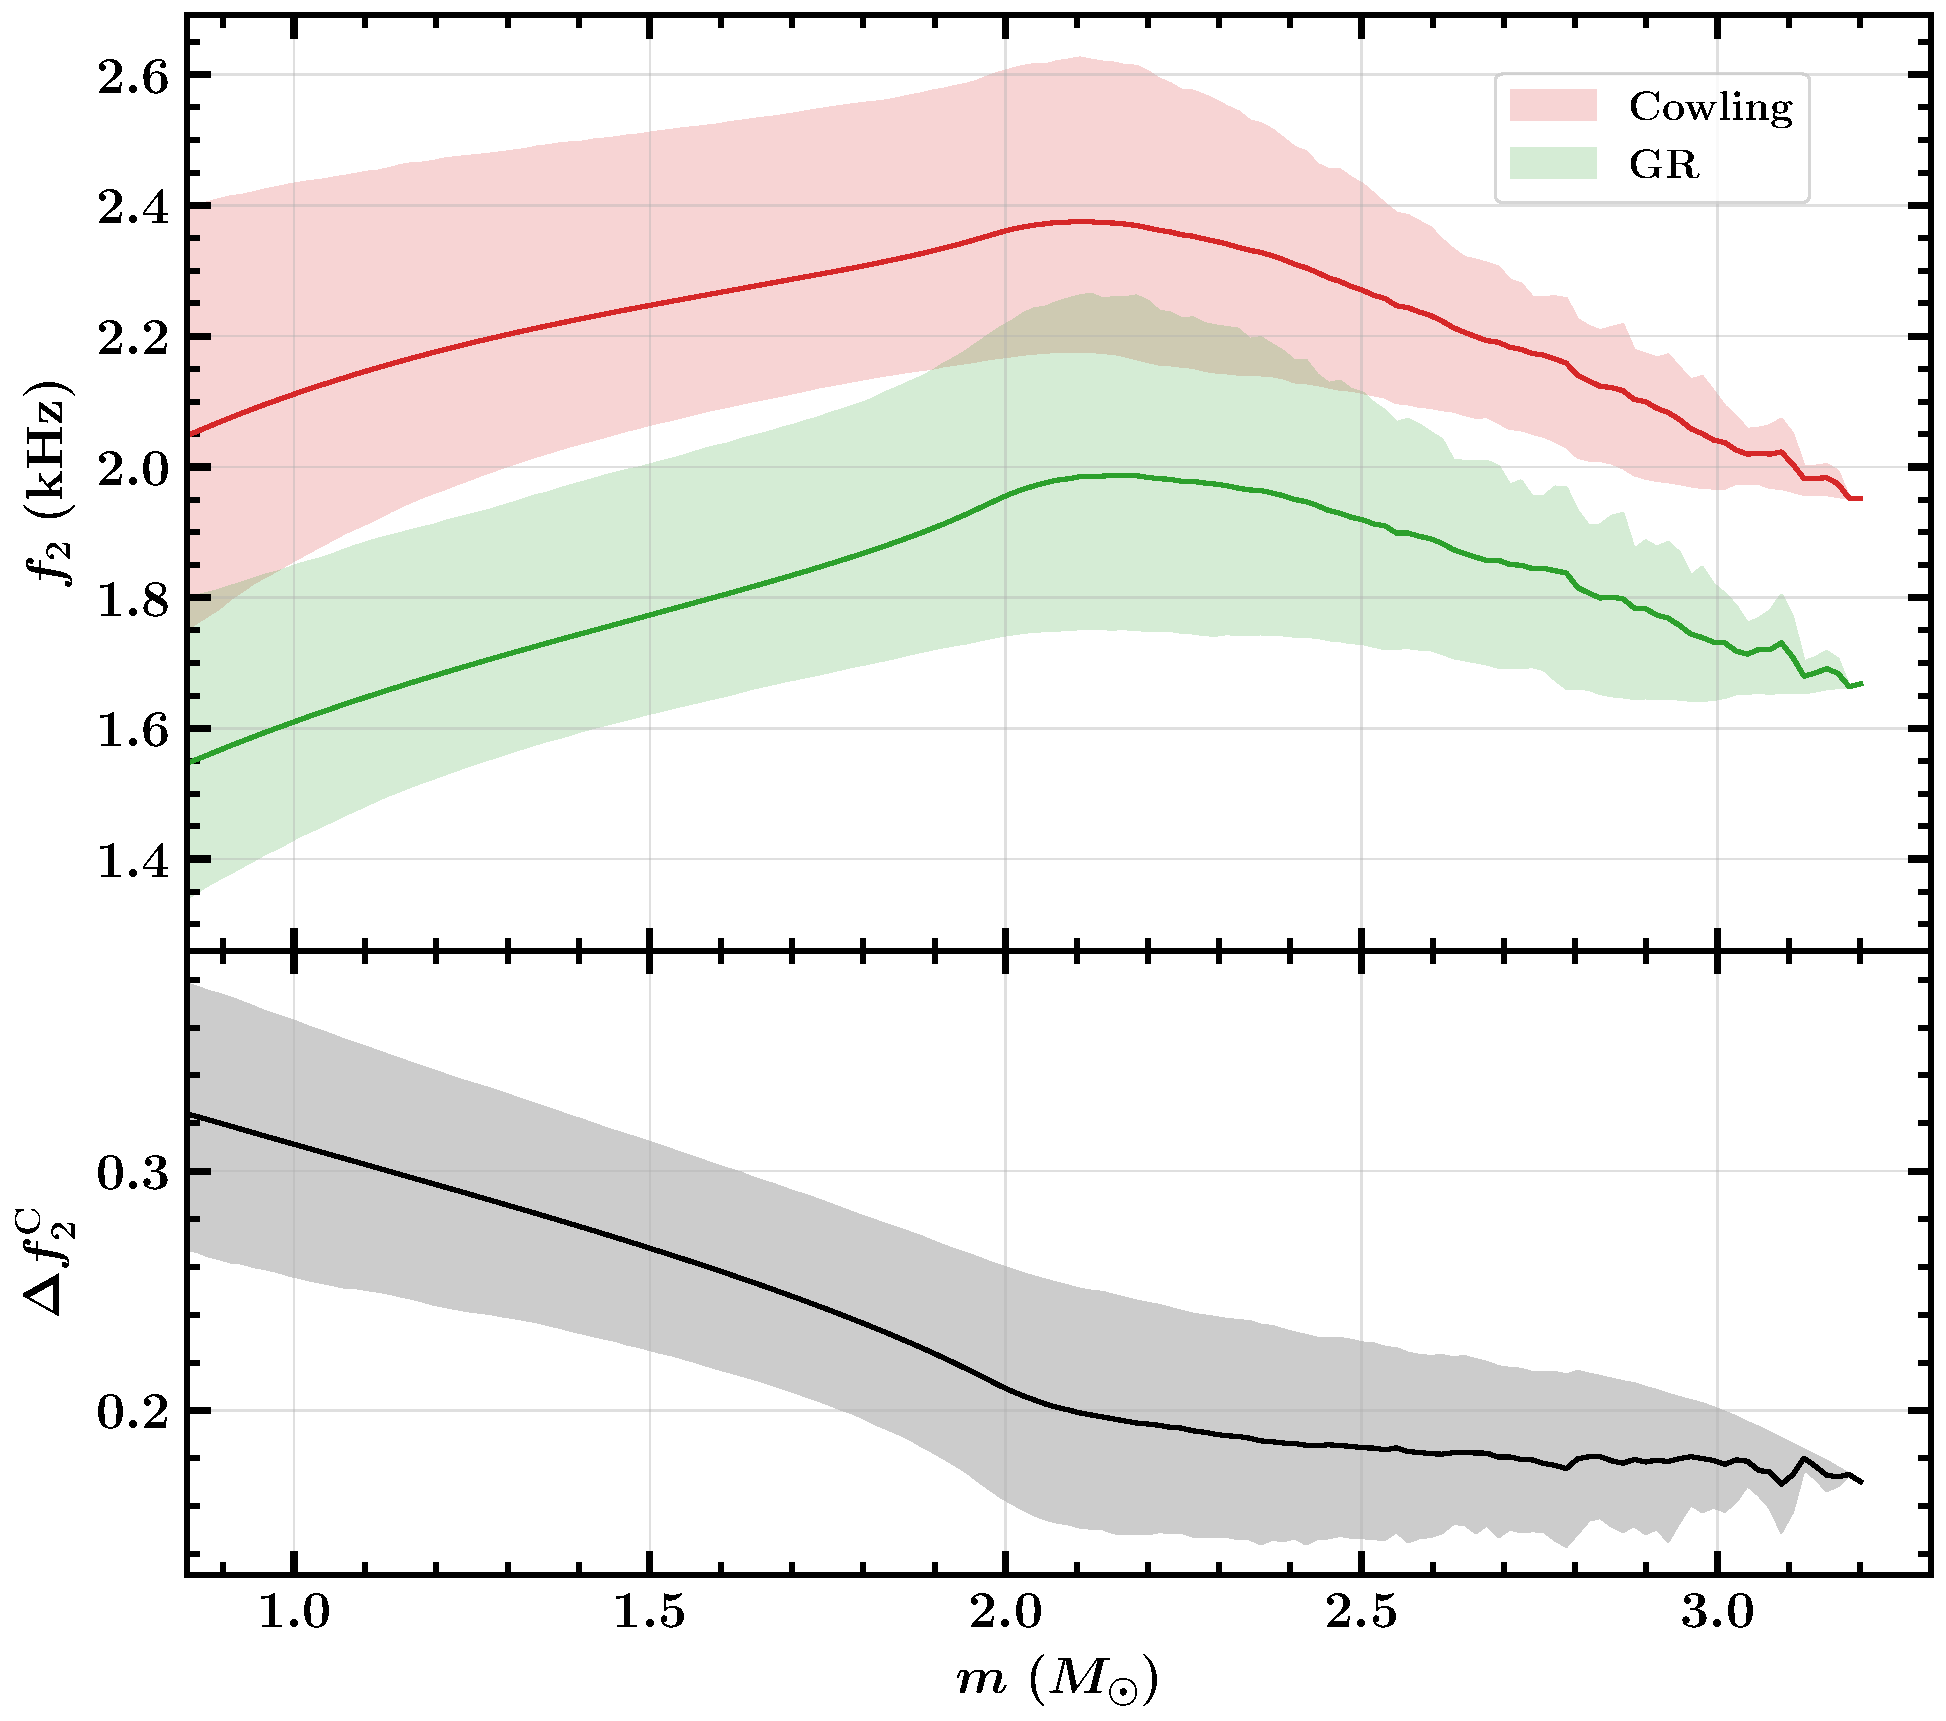
\includegraphics[width=\linewidth]{Cowling/CA_vs_GR_Envelope_plot2.pdf}%
    % 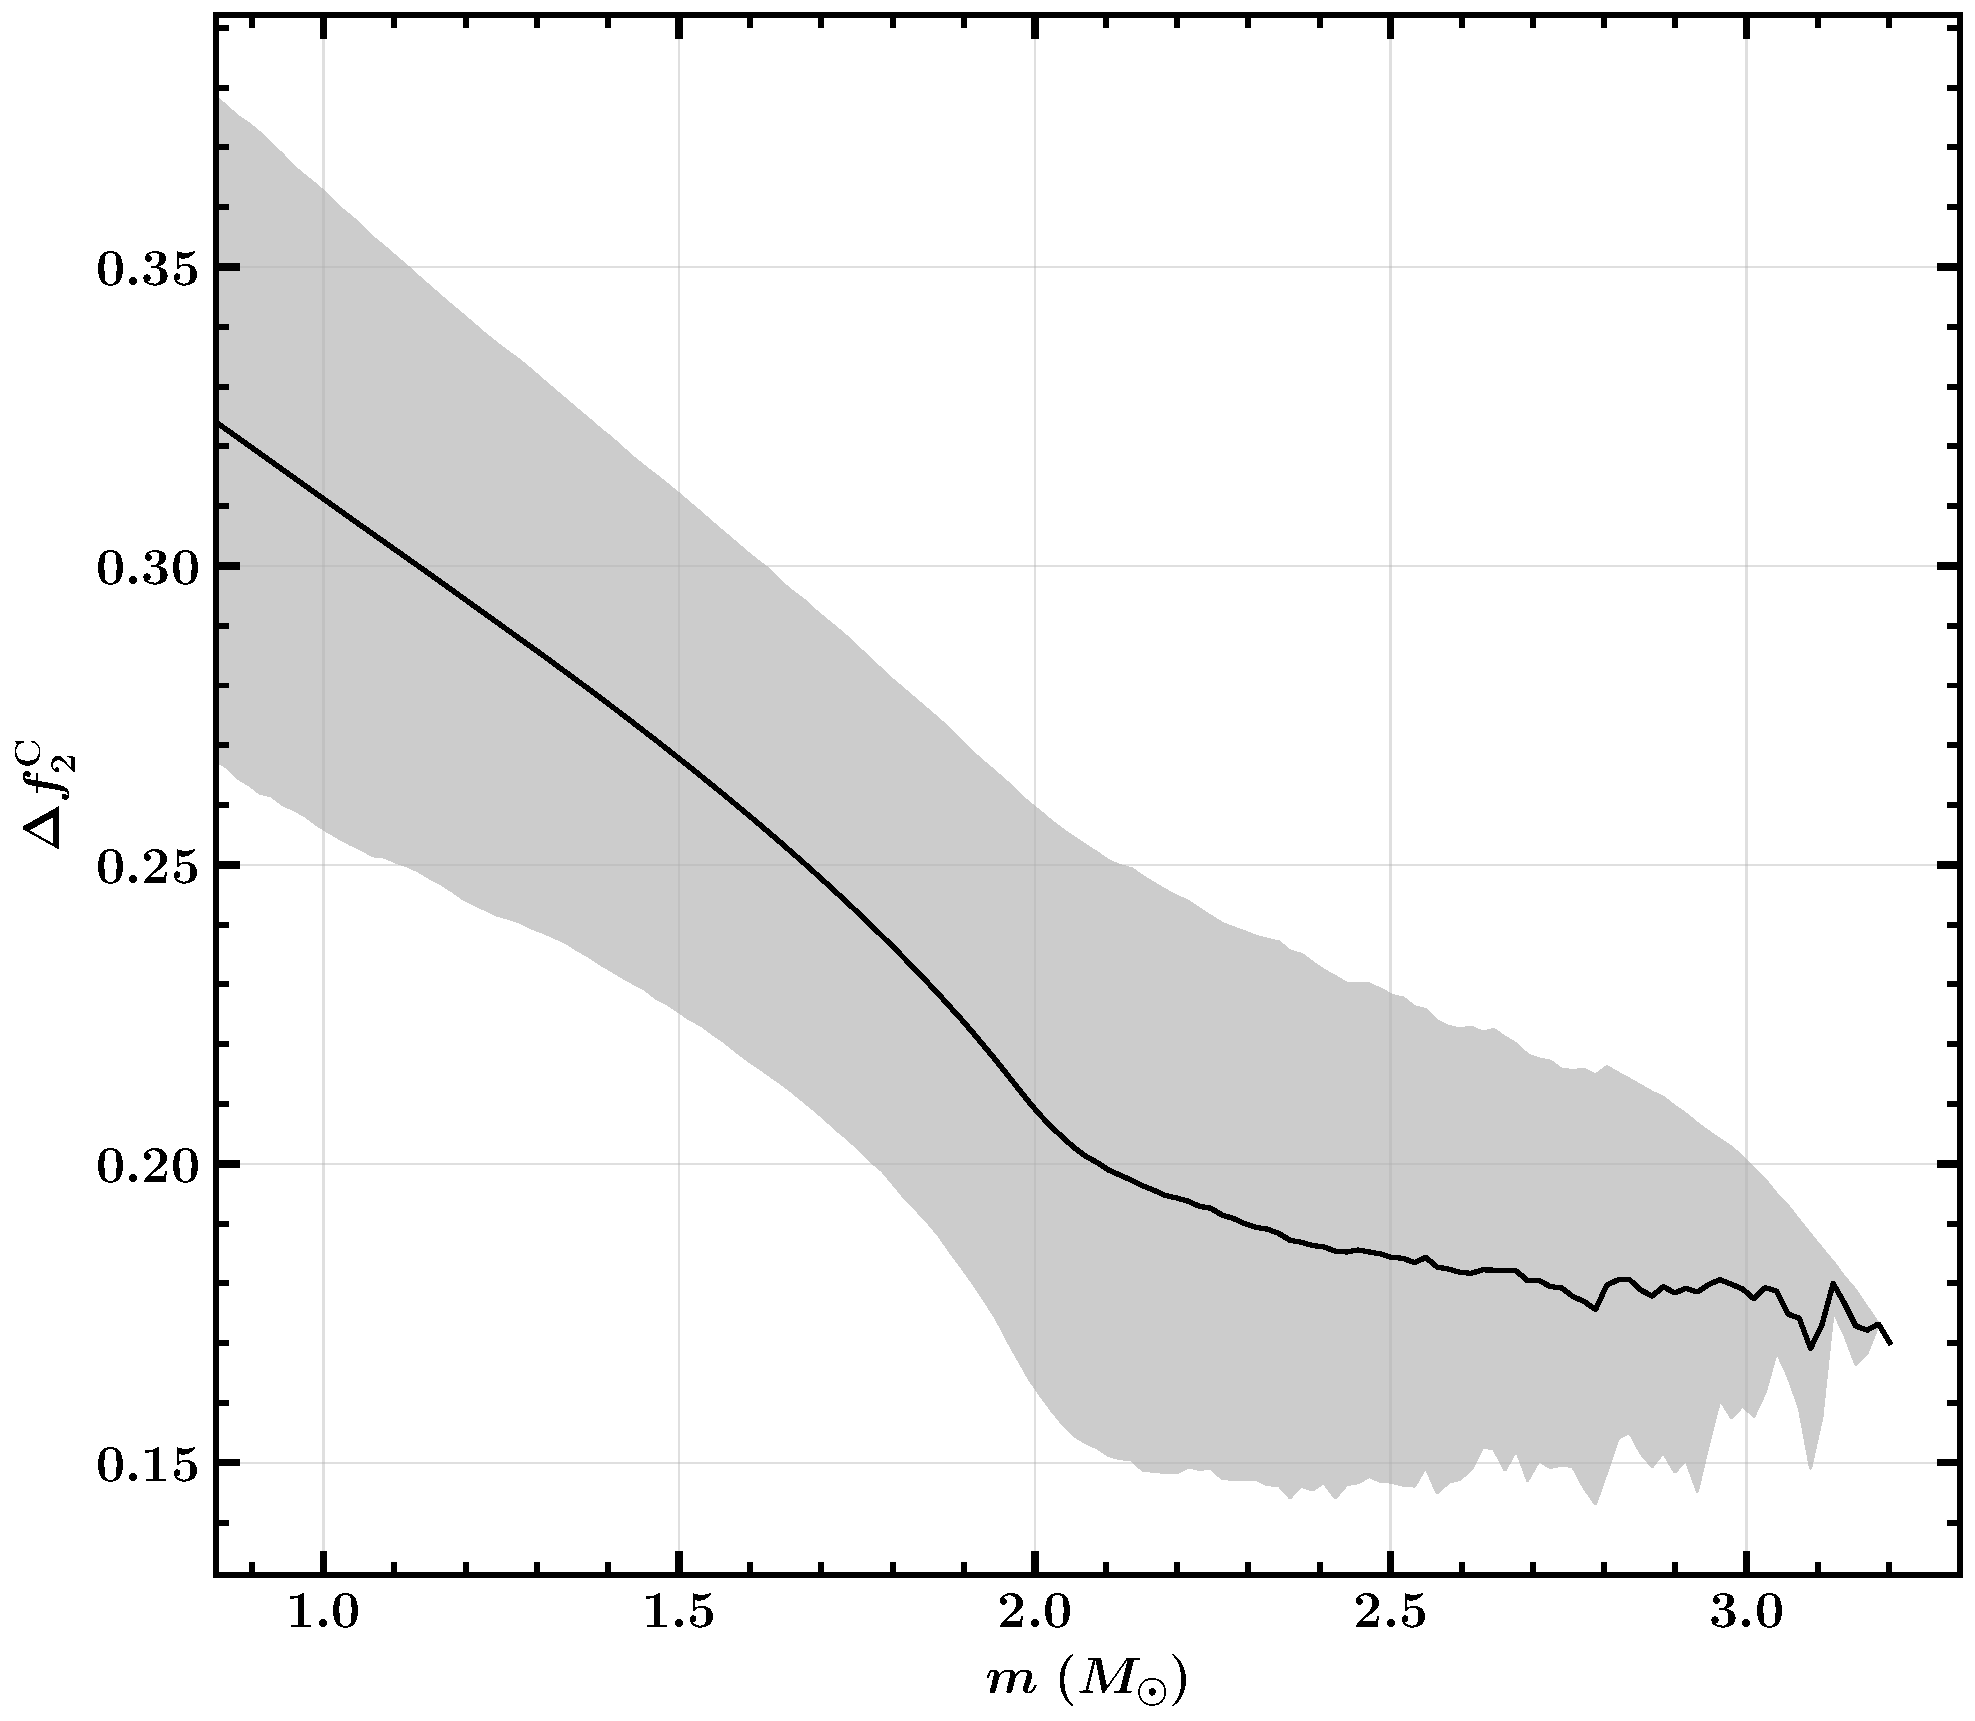
\includegraphics[width=\linewidth]{Cowling/CA_ratio_GR_Envelope_plot.pdf}
    \caption{Comparison between quadrupolar $f$-mode frequencies computed in perturbative general relativity and in the Cowling approximation. The top panel compares the distribution of $f_2(m)$ relations for the PSR+GW+NICER dataset from Fig.~\ref{fig:Envelope Plot} (green) against the corresponding distribution computed in the Cowling approximation (red), with the shaded region encapsulating 90\% credible intervals on $f_2$. The bottom panel shows the fractional difference $\Delta f_2^{\rm C} := (f_2^{\rm C}/f_2 - 1)$ between the perturbative general-relativistic and Cowling results as a function of NS mass, with the shaded region again denoting 90\% credible intervals due to the EOS uncertainty in the PSR+GW+NICER dataset. The discrepancy is larger for lower NS masses.
    }
    \label{fig:cowling1}
\end{figure}
%%%%%%%%%%%%%%

In this study, we conduct a perturbative general-relativistic analysis to compute the fundamental neutron-star oscillation mode. Owing to the significant computational cost associated with this method, a simplified alternative formalism, commonly employed in the literature to determine $f$-mode frequencies, is the Cowling approximation~\cite{cowling1941non, finn1988relativistic}. The Cowling approximation represents a short-wavelength approach that disregards the metric perturbations in the aforementioned Einstein-Euler framework. Consequently, this method involves solving fewer coupled equations and entails reduced computational runtime \cite{lindblom1990accuracy, doneva2012nonradial, samuelsson2007neutron}. It is well-documented that the oscillation mode frequencies derived using the Cowling approximation can deviate from those obtained through general-relativistic calculations by as much as 20\% to 30\%~\cite{yoshida1997accuracy, athulkp}, and tend to systematically overestimate the $f$-mode frequency \cite{Sotani_2020}. This paper delineates the methodology underpinning the Cowling approximation and recomputes the quadrupolar $f$-mode frequencies within this framework to compare its predictions with the general-relativistic results presented in the main body of the paper.

Ignoring the metric perturbations in Eqs. (\ref{odei})–(\ref{odef}), i.e.~enforcing $H_1 = K = H_0 = 0$, we are left with simplified fluid perturbation equations~\cite{2204}:
\begin{align} % requires amsmath; align* for no eq. number
   r\frac{dW}{dr} = & -(l+1) \left[W - l e^{\nu + \lambda/2} U \right] \\ & - \frac{e^{\lambda/2}(\omega r)^2}{c_{ad}^2} \left[U - \frac{e^{\lambda/2}QWc^2}{(\omega r)^2} \right] , \nonumber \\ r \frac{dU}{dr} = & e^{- \nu + \lambda/2 } \left[W - l e^{\nu - \lambda/2} U\right] ,
\end{align}
where we have defined $U = -e^{-\nu}V$. The initial condition for integration of the system starting at $r=0$ is~\cite{2205}
\begin{equation}
\left.\frac{W}{U}\right|_{r=0}=l e^{\nu(r=0)} ,
\end{equation}
where $\nu(r=0)$ is determined by the background TOV solution and $W(r=0)$ is arbitrary; the $f$-mode frequency depends only on the ratio $W/U$. For quadrupolar $f$-modes, we specialize to $\ell = 2$ and integrate numerically from $r=0$ to the stellar surface $r=R$. The oscillation mode frequency $\omega$ is computed by optimizing the following boundary conditions at the stellar surface:%, for which we use the Nelder-Mead minimizer~\cite{} \PL{need a cite here}:
\begin{equation}
\left.\frac{W}{U}\right|_{r=R}=\frac{\omega^{2} R^{3}}{G M} \sqrt{1-\frac{2 G M}{c^{2} R}}
\end{equation}
As in the main text, this procedure is repeated on a grid of neutron star configurations for each EOS in the PSR, PSR+GW and PSR+GW+NICER datasets to build up a posterior distribution over $f_2(m)$ relations.

We compare the distribution of quadrupolar $f$-mode frequency vs mass relations obtained within the Cowling approximation to that computed in perturbative general relativity in Fig.~\ref{fig:cowling1}. As shown in the top panel, the quadrupolar $f$-mode frequencies computed in the Cowling approximation are consistently higher across the neutron star mass spectrum when conditioned on the PSR+GW+NICER dataset. For instance, at a canonical neutron star mass of $ 1.4 \, M_\odot $, the Cowling approximation predicts $ f_{1.4} \approx 2.23^{+0.27}_{-0.19}$ kHz, whereas the general-relativistic calculation estimates $ f_{1.4} \approx 1.75^{+0.23}_{-0.15}$ kHz, a discrepancy of about 28\%. The discrepancy becomes less pronounced at higher neutron star masses. For $ 2.5 \, M_\odot $ neutron stars, the Cowling approximation estimates an $f_2$ value of $2.27^{+0.16}_{-0.16}$ kHz, while the fully relativistic calculation yields $f_2 \approx$ $1.92^{+0.19}_{-0.19}$ kHz, for an 18\% deviation. The lower panel of Fig.~\ref{fig:cowling1} further illustrates this point by showing the fractional difference between the quadrupolar $f$-mode frequency in the Cowling approximation and the perturbative general-relativistic calculation, denoted as $\Delta f_2^{\rm C} := (f_2^{\rm C}/f_2 - 1)$.  These discrepancies highlight the importance of metric perturbations for accurate determination of $f$-mode frequencies, especially for more compact neutron stars where relativistic effects are more important. %\PL{I commented out the last paragraph, which seemed redundant, but there are some stats in there that might address my comment above about quoting exact numbers}

%The lower panel of Fig.~\ref{fig:cowling1} further illustrates this point by showing the fractional difference between the quadrupolar $f$-mode frequency in the Cowling approximation and the perturbative general-relativistic calculation, denoted as $\Delta f_2^{\rm C} := (f_2^{\rm C}/f_2 - 1)$. This ratio is around 0.32 for lower-mass neutron stars (of approximately $ 1.0 \, M_\odot $) and gradually decreases to about 0.17 for masses of $ 3.0 \, M_\odot $. This indicates that the Cowling approximation overestimates the $ f $-mode frequency by approximately 18-25\% at lower masses, with the discrepancy decreasing to about 12-18\% as the mass increases. At 90\% credibility, the error between the two methods at any mass is at least 12\%. For a typical NS mass, 1.4 $M_{\odot}$, this number rises to a minimum error of 18\% at 90\% confidence. The closing deviation from zero with mass underscores the increasing reliability of the Cowling approximation for more massive neutron stars.
%, whose greater compactnesses imply that relativistic corrections are more important. \PL{[I'm not sure this is what the plot shows]} \PL{[Some discussion is repeated between the last two paragraphs, they should be condensed (and made to agree where they say opposite things)]}

\begin{comment}
\begin{figure}[h]
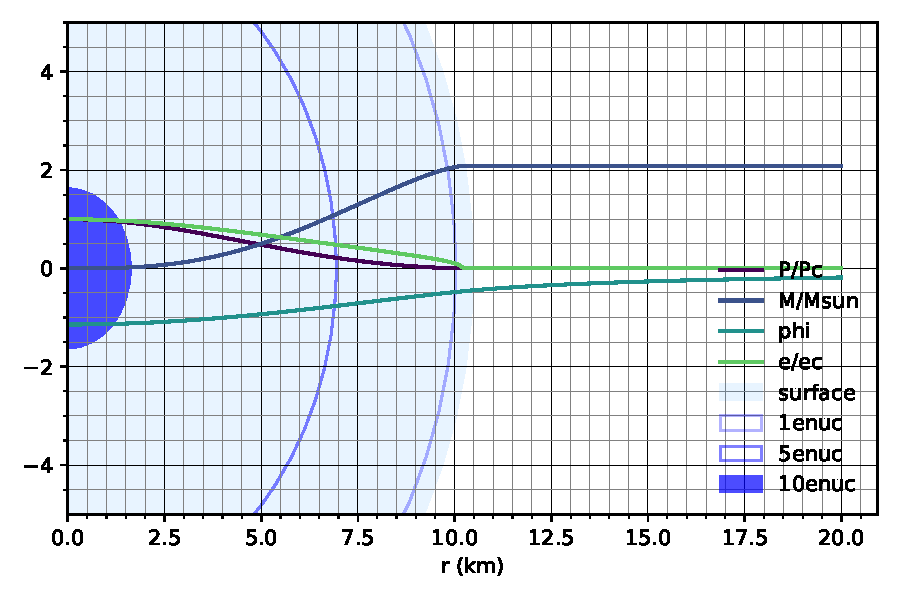
\includegraphics[width=0.5\textwidth]{utkarsh_images/ns_params_overplot.pdf}
\caption{\label{fig:2} NS Structure Overplot [Placeholder]}
\end{figure}

\begin{figure}[h]
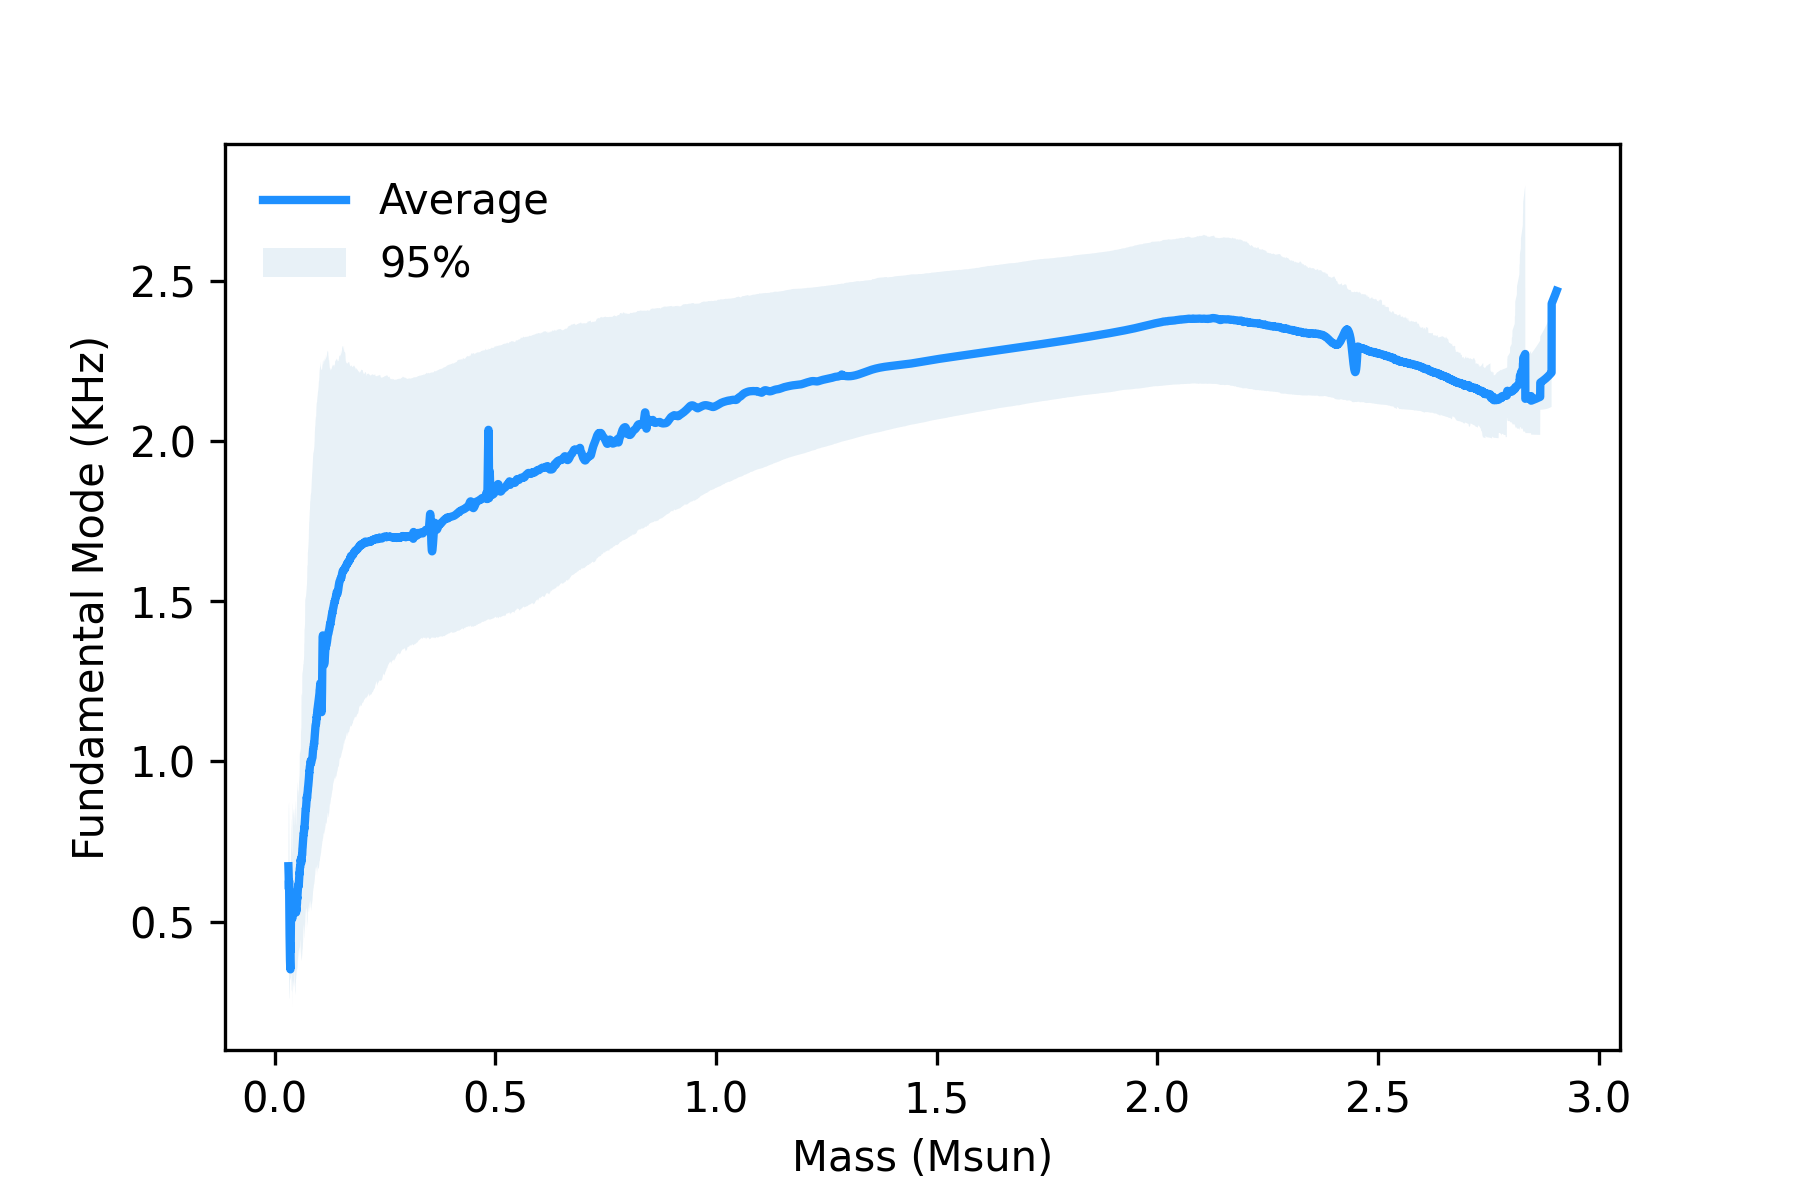
\includegraphics[width=0.5\textwidth]{utkarsh_images/fmode_envelope.png}
\caption{\label{fig:3} Envelope plot of fundamental modes in cowling approximation. 95\% confidence interval is shown. [Cowling Approximation]}
\end{figure}
\begin{figure}[h]
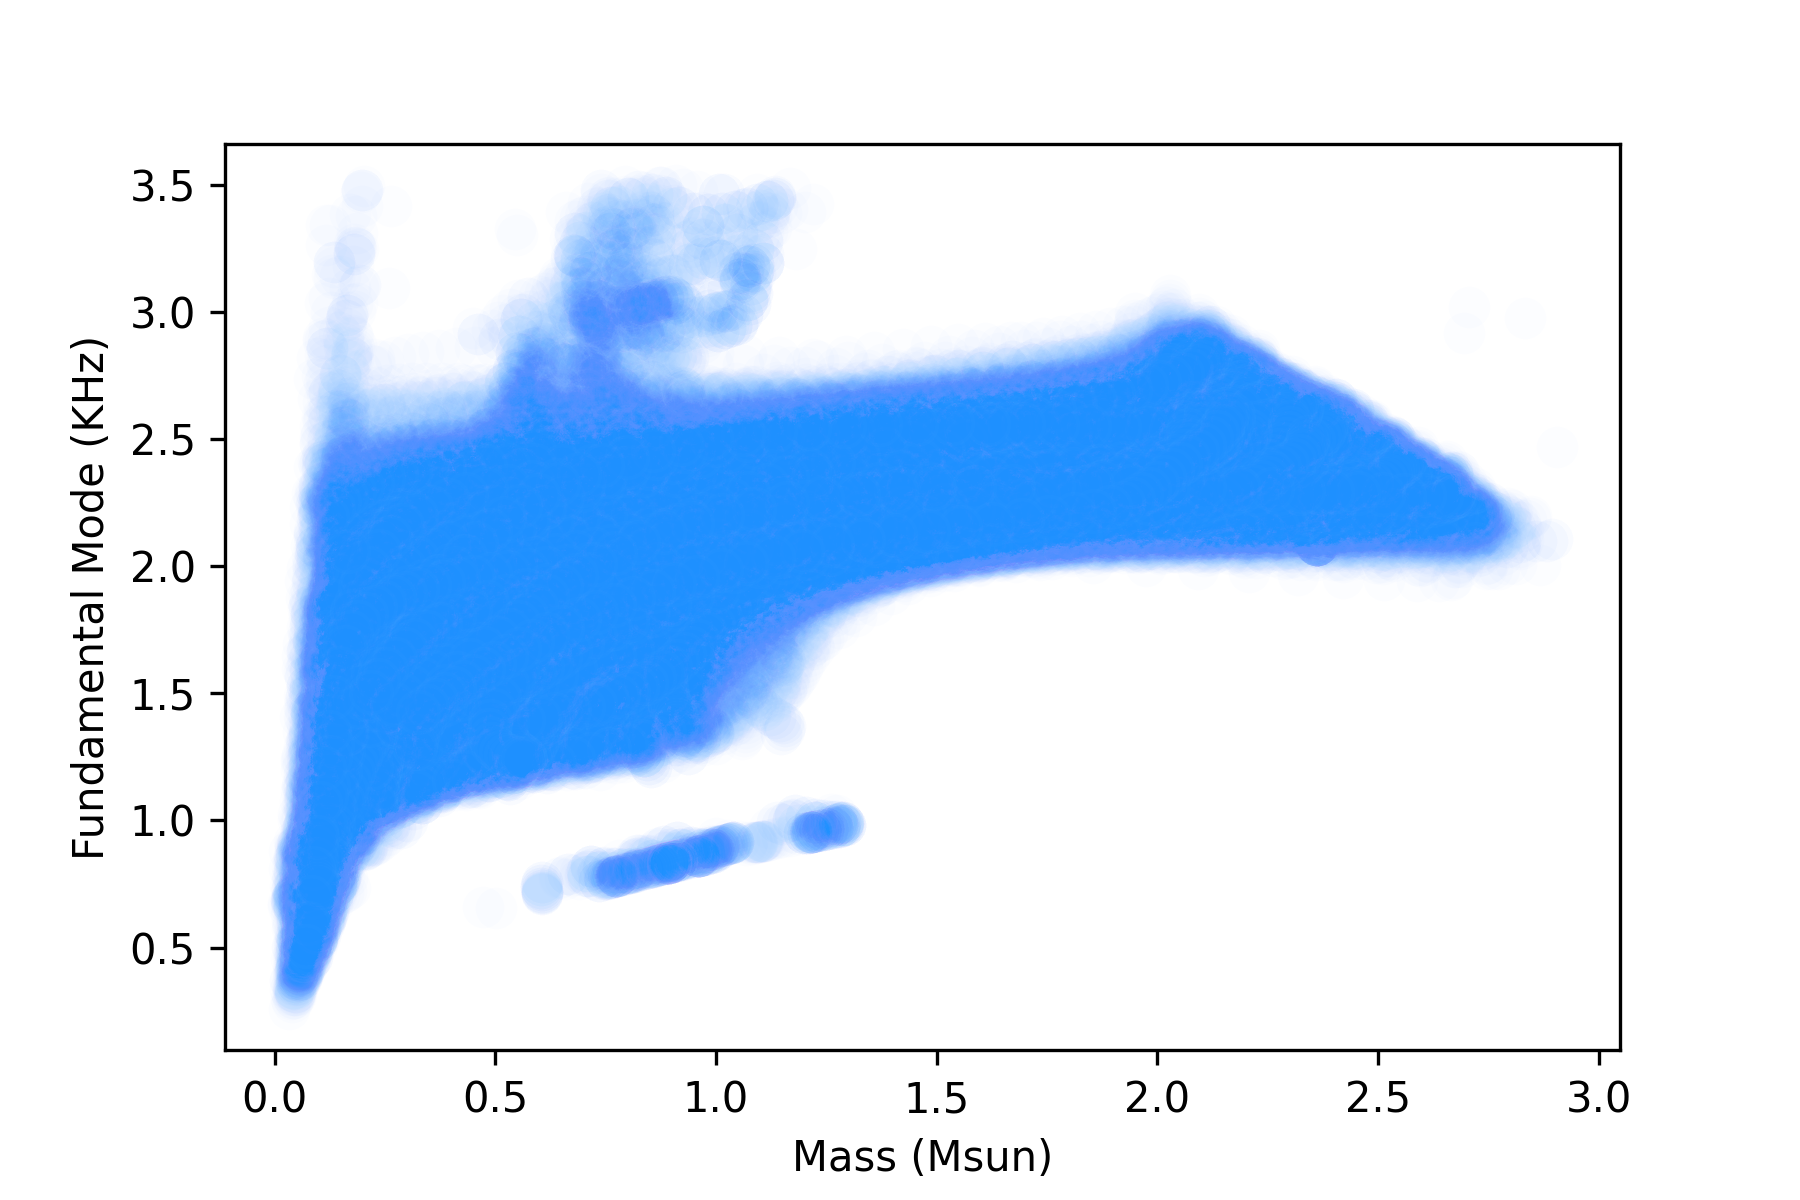
\includegraphics[width=0.5\textwidth]{utkarsh_images/fmode_scatter.png}
\caption{\label{fig:4} Scatter plot for fundamental modes vs mass relationship. Shaded region highlights high concentration of fmode vs mass relation. [Cowling Approximation]}
\end{figure}
\begin{figure}[h]
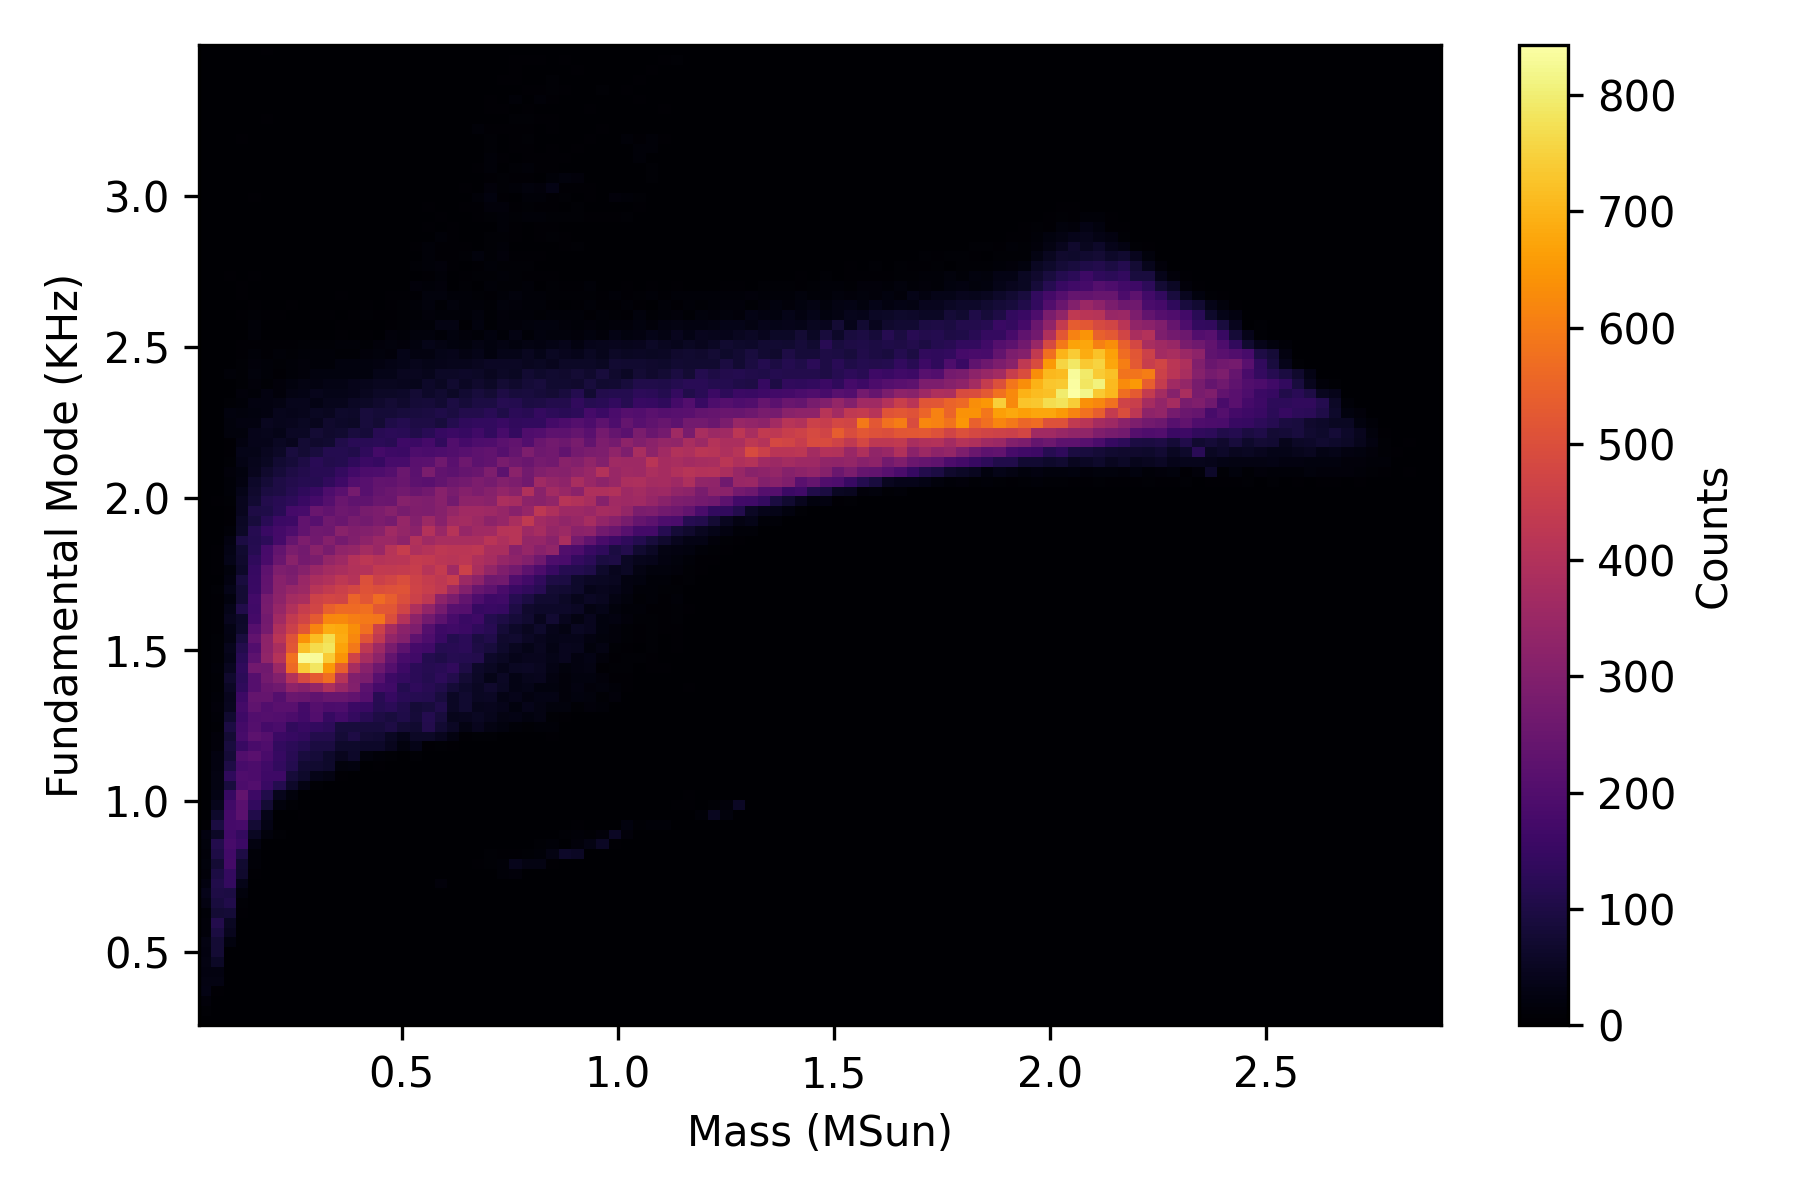
\includegraphics[width=0.5\textwidth]{utkarsh_images/fmode_bins.png}
\caption{\label{fig:5} Bins plot of fundamental mode vs mass of neutron star. Highlighted regions represent sharper concentration. [Cowling Approximation]}
\end{figure}
\begin{figure}[h]
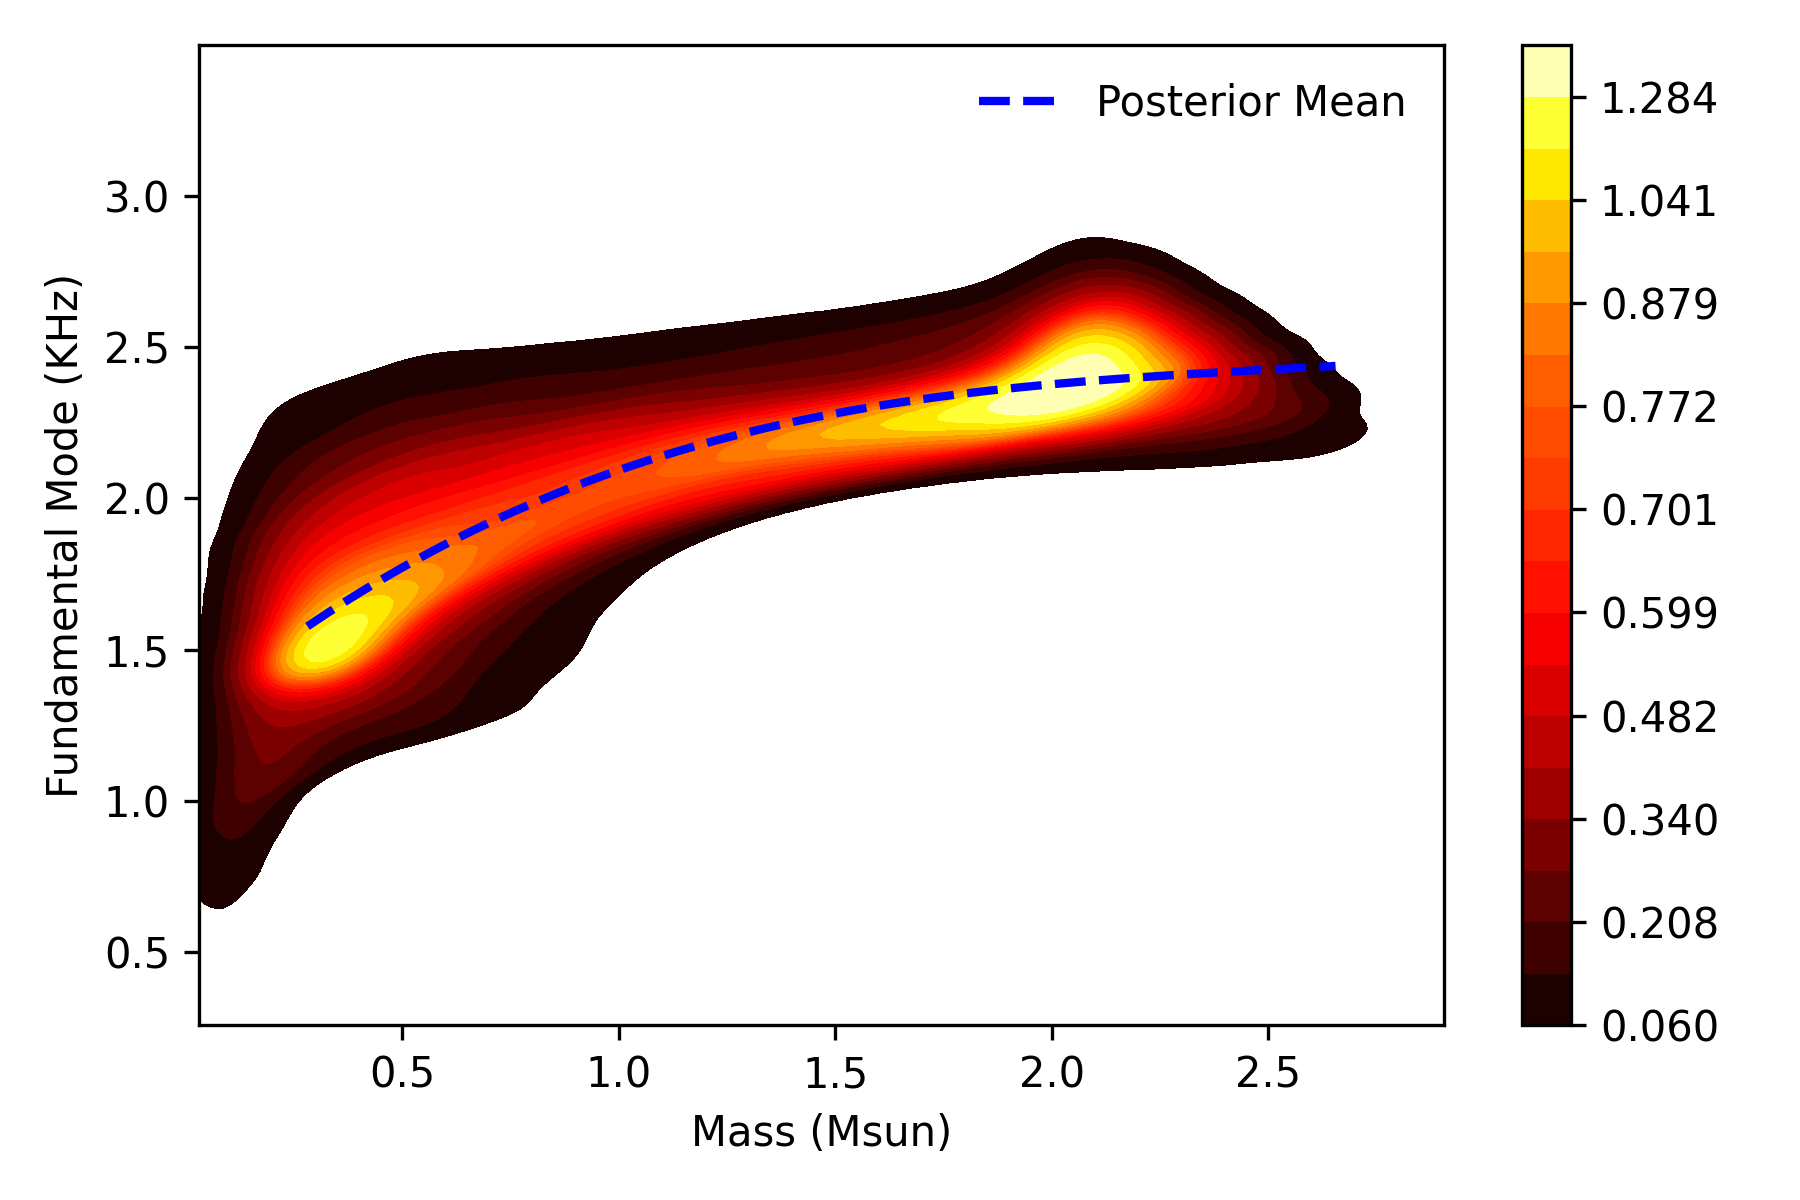
\includegraphics[width=0.5\textwidth]{utkarsh_images/fmode_contour.png}
\caption{\label{fig:6} Contour plot of fmode vs mass in the cowling approximation with the posterior mean over plotted. Lighted colours represent higher densities. [Cowling Approximation]} 
\end{figure}
\begin{figure}[h]
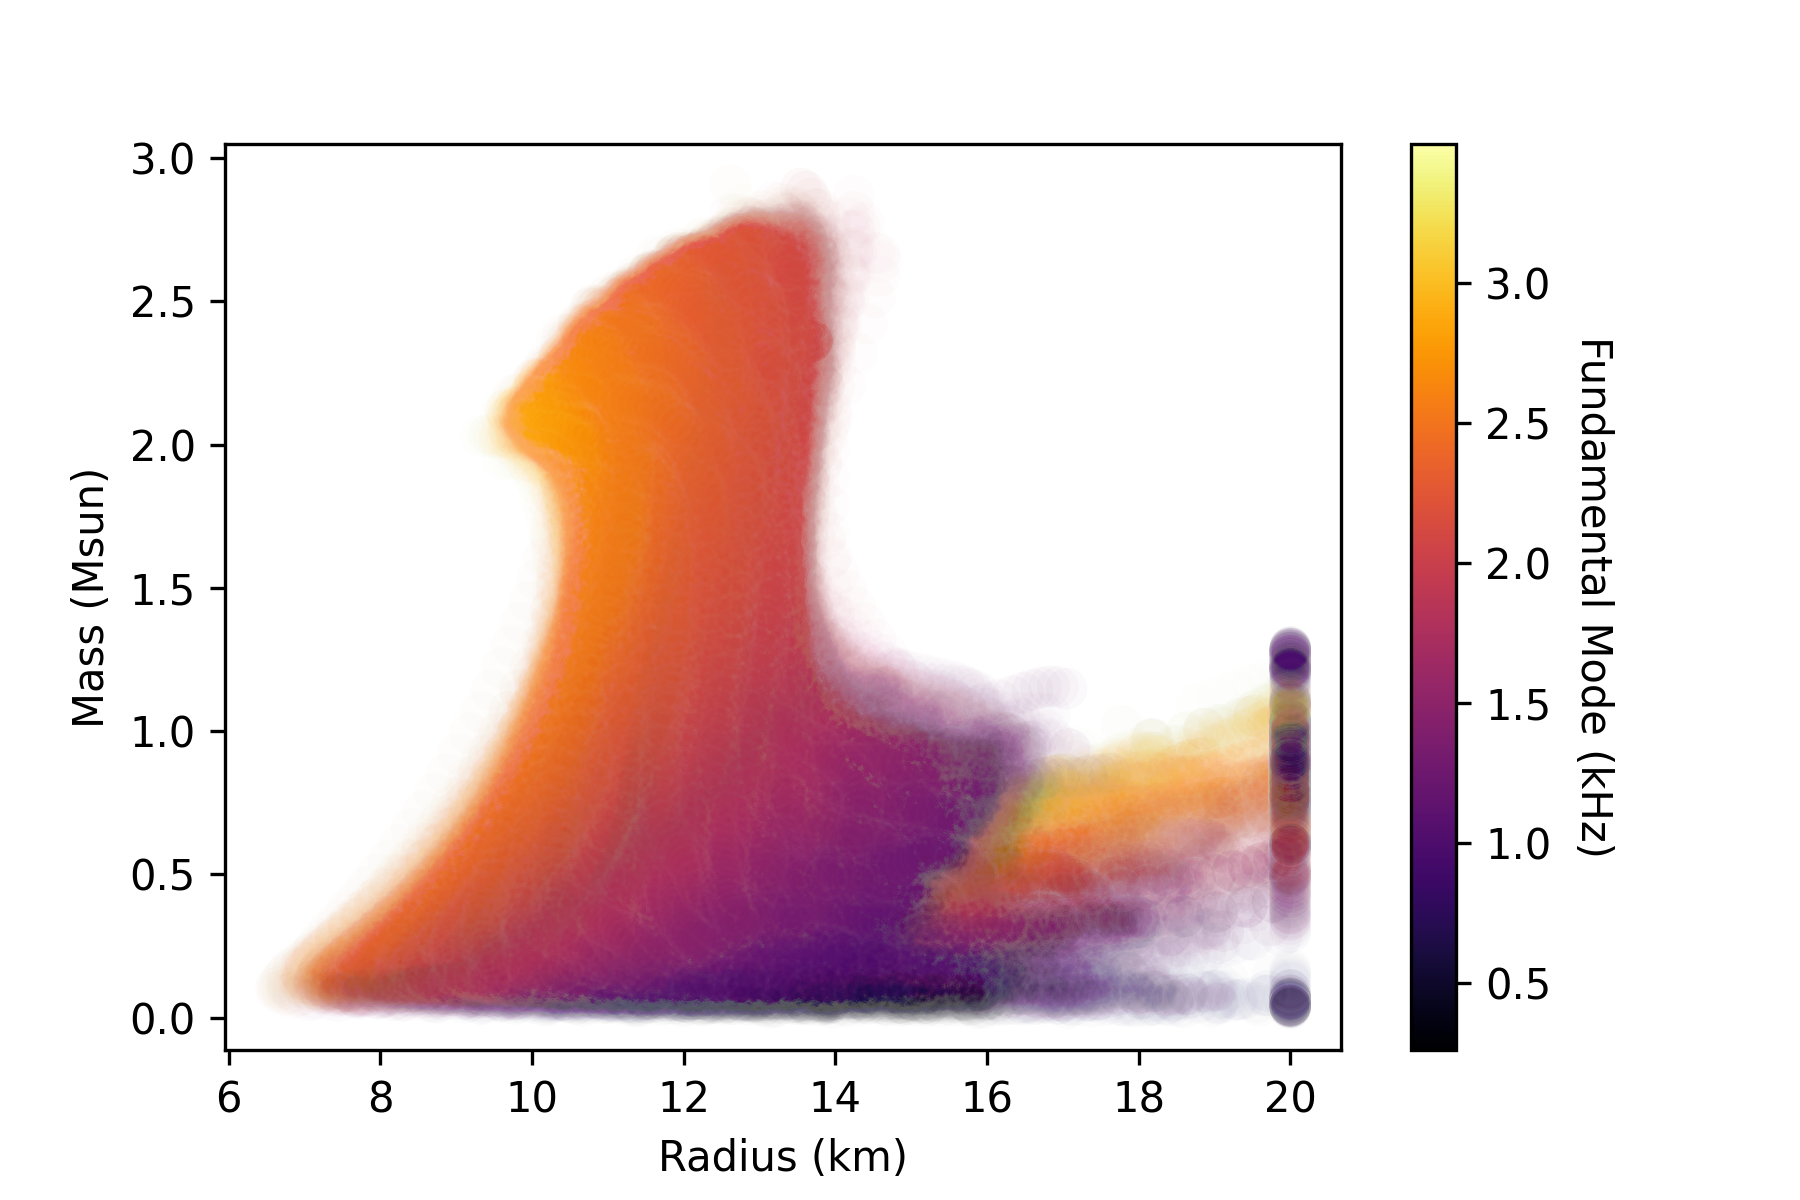
\includegraphics[width=0.5\textwidth]{utkarsh_images/fmode_MR.png}
\caption{\label{fig:7} Fundamental mode mass radius relationship with colour schematic of fundamental modes in the cowling approximation. Models drawn from EOS data. [Cowling Approximation]}
\end{figure}
\end{comment}

%Figure \ref {fig:cowling2} presents the PDFs for the recovery of specific $ f $-mode frequencies using the Cowling approximation (dashed lines) and fully relativistic (GR) calculations (solid lines) across various neutron star masses. In the left panel, the figure compares the $ f $-mode PDFs for the primary and secondary components of two observed  BNS merger events: GW170817 and GW190425. The right panel contrasts the $ f $-mode PDFs for neutron stars at maximum mass (in red) and canonical mass (in orange), again showing both the Cowling approximation and fully relativistic results. For the GW170817 event, the $ f $-mode frequencies predicted by the fully relativistic model are centered around 2.0 kHz for the primary component (blue solid line) and approximately 2.2 kHz for the secondary component (orange solid line). In contrast, the Cowling approximation predicts slightly higher frequencies, around 2.1 kHz and 2.3 kHz for the primary and secondary components, respectively. This corresponds to a deviation of about 5\% to 10\% between the two models, reinforcing the trend that the Cowling approximation tends to overestimate the $ f $-mode frequency. Similar discrepancies are observed in the GW190425 event, where the fully relativistic approach yields frequencies around 1.6 kHz and 1.9 kHz for the primary and secondary components (green and red solid lines), while the Cowling approximation predicts higher values around 1.7 kHz and 2.0 kHz, indicating a deviation in the same range.

%The right panel further emphasizes the differences between these two approaches by focusing on neutron stars with canonical and maximum masses. For a canonical neutron star mass of $ 1.4 \, M_\odot $, the fully relativistic model predicts an $ f $-mode frequency around 1.8 kHz, whereas the Cowling approximation suggests a frequency closer to 2.0 kHz. The difference here is approximately 11\%. For maximum mass neutron stars, the discrepancy widens, with the fully relativistic model predicting a frequency around 2.4 kHz and the Cowling approximation yielding a frequency of nearly 2.7 kHz, marking a deviation of approximately 12.5\%. These differences are particularly significant for gravitational wave detections, as they underscore the necessity of using fully relativistic calculations to achieve accurate modeling of the $ f $-mode frequencies, which are critical for waveform analysis and interpretation in gravitational wave observatories.

%Results comparing the methods applied to the BNS mergers GW170817 and GW190425 are shown in Figure \ref{fig:cowling2}. The left panel highlights the f-modes for all component masses. Of the observed events, the most common f-mode lies between $1.5-1.9$ kHz. While the Cowling approximation is inaccurate, it did not change the ordering of the f-mode values in component masses. This suggests that the Cowling approximation produces systematically biased f-modes. The right panel in Figure \ref{fig:cowling2} supports our claim of a larger f-mode error in smaller-mass neutron stars. We note that the posterior on a canonical mass NS might be tighter than that of the maximum mass NS. \UM{Why would this be the case?}
%%%%%%%%%%%%%%

\clearpage
%%%%%%%%%%%%%%%%%%%%%
\bibliographystyle{apsrev4-1}
\bibliography{references}
%%%%%%%%%%%%%%%%%%%%%
\end{document}
%%%%%%%%%%%%%%%%%%%%%